%% Copernicus Publications Manuscript Preparation Template for LaTeX Submissions
%% ---------------------------------
%% This template should be used for copernicus.cls
%% The class file and some style files are bundled in the Copernicus Latex Package, which can be downloaded from the different journal webpages.
%% For further assistance please contact Copernicus Publications at: production@copernicus.org
%% https://publications.copernicus.org/for_authors/manuscript_preparation.html


%% Please use the following documentclass and journal abbreviations for preprints and final revised papers.

%% 2-column papers and preprints
\documentclass[journal abbreviation, manuscript]{copernicus}

%% Journal abbreviations (please use the same for preprints and final revised papers)

% Advances in Geosciences (adgeo)
% Advances in Radio Science (ars)
% Advances in Science and Research (asr)
% Advances in Statistical Climatology, Meteorology and Oceanography (ascmo)
% Aerosol Research (ar)
% Annales Geophysicae (angeo)
% Archives Animal Breeding (aab)
% Atmospheric Chemistry and Physics (acp)
% Atmospheric Measurement Techniques (amt)
% Biogeosciences (bg)
% Climate of the Past (cp)
% DEUQUA Special Publications (deuquasp)
% Earth Surface Dynamics (esurf)
% Earth System Dynamics (esd)
% Earth System Science Data (essd)
% E&G Quaternary Science Journal (egqsj)
% EGUsphere (egusphere) | This is only for EGUsphere preprints submitted without relation to an EGU journal.
% European Journal of Mineralogy (ejm)
% Fossil Record (fr)
% Geochronology (gchron)
% Geographica Helvetica (gh)
% Geoscience Communication (gc)
% Geoscientific Instrumentation, Methods and Data Systems (gi)
% Geoscientific Model Development (gmd)
% History of Geo- and Space Sciences (hgss)
% Hydrology and Earth System Sciences (hess)
% Journal of Bone and Joint Infection (jbji)
% Journal of Micropalaeontology (jm)
% Journal of Sensors and Sensor Systems (jsss)
% Magnetic Resonance (mr)
% Mechanical Sciences (ms)
% Natural Hazards and Earth System Sciences (nhess)
% Nonlinear Processes in Geophysics (npg)
% Ocean Science (os)
% Polarforschung - Journal of the German Society for Polar Research (polf)
% Primate Biology (pb)
% Proceedings of the International Association of Hydrological Sciences (piahs)
% Safety of Nuclear Waste Disposal (sand)
% Scientific Drilling (sd)
% SOIL (soil)
% Solid Earth (se)
% State of the Planet (sp)
% The Cryosphere (tc)
% Weather and Climate Dynamics (wcd)
% Web Ecology (we)
% Wind Energy Science (wes)


% \usepackage commands included in the copernicus.cls:1
% \usepackage[german, english]{babel}
% \usepackage{tabularx}
% \usepackage{cancel}
% \usepackage{multirow}
% \usepackage{supertabular}
% \usepackage{algorithmic}
% \usepackage{algorithm}
% \usepackage{amsthm}
% \usepackage{float}
% \usepackage{subfig}
% \usepackage{rotating}
\usepackage{booktabs}
\usepackage{multirow}

\usepackage{graphicx}
\usepackage{subcaption}
\usepackage{tablefootnote} % for table footnotes
\usepackage{alphalph}

\usepackage{tikz}
\usetikzlibrary{shapes.geometric, positioning, fit, backgrounds,matrix, arrows.meta}

\tikzstyle{startstop} = [rectangle, rounded corners, 
minimum width=1cm, 
minimum height=1cm,
text centered, 
text width=4cm,
draw=black, 
fill=red!30]

% \tikzstyle{io} = [trapezium, 
% trapezium stretches=true, % A later addition
% trapezium left angle=70, 
% trapezium right angle=110, 
% minimum width=3cm, 
% minimum height=1cm, text centered, 
% draw=black, fill=blue!30]

\tikzstyle{process} = [rectangle, 
minimum width=5cm, 
minimum height=1cm, 
text centered, 
text width=4cm, 
draw=black, 
fill=orange!30
]

\tikzstyle{classify} = [rectangle, 
minimum width=5cm, 
minimum height=1cm, 
text centered, 
text width=4cm, 
draw=black, 
fill=blue!30
]

\tikzstyle{decision} = [diamond, 
minimum width=3cm, 
minimum height=1cm, 
text centered, 
draw=black, 
fill=green!30]
\tikzstyle{arrow} = [thick,->,>=stealth]


\renewcommand{\thefootnote}{\alphalph{\value{footnote}}}

\begin{document}

\title{6-year statistical analysis of cloud occurrence and its physical properties using ACTRIS-CCRES remote sensing data}


% \Author[affil]{given_name}{surname}

\Author[1,2][mtolentino@ugr.es]{M.}{Tolentino} %% correspondence author
\Author[1,2]{J.A.}{Bravo-Aranda}
\Author[1,2]{M.J.}{Granados-Muñoz}
\Author[1,2]{J.L.}{Guerrero-Rascado}
\Author[1,2]{L.}{Alados-Arboledas}

\affil[1]{Department of Applied Physics, University of Granada, Granada, 18072, Spain}
\affil[2]{Andalusian Institute for Earth System Research, Granada (IISTA-CEAMA), 18006, Spain}
%\affil[]{ADDRESS}
%\affil[]{ADDRESS}
%\affil[]{ADDRESS}

%% The [] brackets identify the author with the corresponding affiliation. 1, 2, 3, etc. should be inserted.

%% If an author is deceased, please mark the respective author name(s) with a dagger, e.g. "\Author[2,$\dag$]{Anton}{Smith}", and add a further "\affil[$\dag$]{deceased, 1 July 2019}".

%% If authors contributed equally, please mark the respective author names with an asterisk, e.g. "\Author[2,*]{Anton}{Smith}" and "\Author[3,*]{Bradley}{Miller}" and add a further affiliation: "\affil[*]{These authors contributed equally to this work.}".


\runningtitle{Cloud properties in Southeast of Spain: a 6-year statistical study using ACTRIS-CCRES remote sensing measurements
}

\runningauthor{TEXT}

\received{}
\pubdiscuss{} %% only important for two-stage journals
\revised{}
\accepted{}
\published{}

%% These dates will be inserted by Copernicus Publications during the typesetting process.


\firstpage{1}

\maketitle


\begin{abstract}

Understanding climate change relies heavily on grasping the role of cloud radiative effect and its climate feedback. However, these factors pose the greatest uncertainty among atmospheric processes. This uncertainty stems partly from the limited global-scale cloud measurements. To address this gap, our study presents a six-year statistical analysis of cloud coverage and microphysics properties at the ACTRIS-CCRES AGORA observatory in Granada, Spain. Here, we utilized CLOUDNET post-processed data (e.g target classification, liquid water path, droplet effective radius and so on) of remote sensing instruments and microwave radiometer thermodynamic profiles. The analysis focuses on single layer cloud properties comparison for liquid, ice, mixed phase, liquid with rain, and mixed phase with rain clouds. Therefore, a distinct seasonal pattern in cloud occurrence was observed. During the summer (June-August), single layer clouds occurrence is less than 10\%, and precipitation is absent. Conversely, cloud occurrence significantly increases during winter (December-February) and spring (March-May), where Ice and mixed phase clouds with rain are the predominant type. Additionally, a negligible presence of liquid clouds with rain were found. Seasonal trends in liquid water content (LWC) and droplet effective radius are unclear for mixed-phase and liquid clouds. Effective radius remains stable year-round, around 5 μm for liquid clouds below 3 km, while for mixed-phase clouds it can vary between 5 and 12 μm, mainly found at 1-2 km and 5-9 km. LWC shows higher values in cold periods and lower in summer, but with significant variability across both cloud types. Same seasonal patterns for ice water content (IWC) in ice and mixed-phase clouds were challenging to identify. Monthly profiles showed little variation, although values tended to rise in summer. Ice clouds typically have effective radius between 20-30 μm at 8-12 km altitude, peaking at 65 μm in summer. Mixed-phase clouds exhibit ice effective radius around 50 μm between 1-7 km altitude. The mean geometric thickness of ice and mixed-phase clouds throughout the seasons is 1.2 ± 1.3 km and 2.0 ± 1.6 km, respectively, contrasting sharply with the 0.2 ± 0.2 km observed in liquid clouds. The monthly variability in thickness is substantial enough to obscure any seasonal differences. Similarly, the analysis of cloud base height reveals mean values of 1.9 ± 2.0 km (excluding summer) for liquid clouds, 4.8 ± 2.2 km for mixed-phase clouds, and 7.0 ± 2.4 km for ice clouds. During summer a different vertical distribution of cloud base was found due to different mechanisms of cloud formation. Conclusively, a statistical analysis was conducted on single-layer cloud properties in the Southeast of Spain, highlighting the mainly cloud type associated with rainfall in the region.

\end{abstract}


\copyrightstatement{TEXT} %% This section is optional and can be used for copyright transfers.


%\section{Introduction}
%Clouds play a vital role in regulating Earth's radiative budget and hydrological cycle. They interact with solar and thermal radiation, affecting the energy balance and, consequently, the surface temperature \citep{twomeyInfluencePollutionShortwave1977, brenguierCloudMicrophysicalRadiative2003, zengModelingRadiativeEffect2021}. Additionally, clouds transport moisture to various regions, being directly associated with drought, which is intensifying in the Mediterranean Region \citep{rios-entenzaMoistureRecyclingIberian2014, hoerlingIncreasedFrequencyMediterranean2012a}. However, studying clouds is quite complex, and their radiative effects are in the spotlight of the atmospheric science community. This challenge arises from clouds' high spatial and temporal variability, as well as the variety of hydrometeor types inside them \citep{intergovernmentalpanelonclimatechangeipccEarthEnergyBudget2023}. The hydrometeor phase, shape and concentration can significantly alter their interaction with solar and thermal radiation \citep{yoshidaEffectsVerticalProfiles2005}, posing a significant challenge to estimate their radiative effect as suggested by \cite{XXX}.


The ground-based remote sensing technique is one of the state-of-the-art methods for measuring clouds. Particularly, the Cloud Doppler Radar (CDR) can perform long-term measurements of clouds, which is one alternative for improving the cloud knowledge. Several studies have been analyzing CDR data in Europe, but they are mostly located in Northern Europe \citep{kneifelMultiyearCloudPrecipitation2022, nomokonovaStatisticsCloudsTheir2019, buhlMeasuringIceLiquidwater2016, achtertPropertiesArcticLiquid2020}. In this context, the AGORA (Andalusian Global ObseRvatory of the Atmosphere) ACTRIS CCRES station has been operating a 94 GHz CDR since 2018, contributing to enhancing the lack of data on the Mediterranean basin, which is a key region for climate variability. This station is one of the southernmost stations that is part of the Cloudnet network \citep{illingworthCloudnet2007}. Notably, it stands as the only cloud remote sensing database available in Spain, making it an invaluable resource for regional climate studies. 
Satellite data would be an alternative to fill the gap of data, but they only provide a general  picture of cloud properties. They present low temporal resolution and information on low level clouds is affected by large uncertainties. Additionally, this data should be validated with the use of ground-based remote sensors such as lidars and CDRs \citep{protatImpactConditionalSampling2006, protatEvaluationCloudSatCALIPSO2010}.
Thus, ground-based observations are still necessary for improving the accuracy of cloud properties.

This study aims to perform a statistical analysis on single layer clouds for more than half a decade of observations at the AGORA station. First, clouds were classified (e.g. ice, liquid or mixed-phase clouds) using the cluster classification algorithm (CBA). This is a novel algorithm that classifies clouds according to the percentage of hydrometeors within each cluster. The clusters are defined using the hydrometeor classification product from Cloudnet.
Second, cloud macrophysics (e.g., cloud thickness, base and top height) and microphysics statistics are performed for each cloud category from CBA. Markedly, cloud statistics in this study are derived from a cluster-based approach, contrasting with previous studies that used the profile-based algorithm (PBA) \citep{pirloagaGroundBasedMeasurementsCloud2022,nomokonovaStatisticsCloudsTheir2019,kneifelMultiyearCloudPrecipitation2022}.
For instance, \cite{nomokonovaStatisticsCloudsTheir2019} used the PBA algorithm to characterize single-layer clouds at the Ny-Ålesund station, \cite{kneifelMultiyearCloudPrecipitation2022} employed it to investigate ice cloud variability in the German Alps, and \cite{pirloagaGroundBasedMeasurementsCloud2022} applied it to examine seasonal cloud variability in Bucharest. \cite{buhlMeasuringIceLiquidwater2016} also uses the PBA but selected intervals with more than 15 min with the same cloud category. On the other hand, the CBA considers the composition of the entire volume occupied by the cloud. \cite{roschkeDiscriminatingDrizzleRain2024} also used the CBA, but with a different classification scheme, separating clusters into warm and cold clouds for the Barbados site. 


The experimental site, datasets, instruments and products are described in Section \ref{sec:site_instruments_products}. The proposed new approach on cloud classification algorithm and the cloud assessment are presented in Section \ref{sec:classification_algorithm}. Section \ref{sec:results} analyzes the annual, seasonal, and daily cycle of cloud types, as well as the base and top height, and thickness. In addition, this section discusses the liquid and ice properties variability for different clouds. Finally, Section \ref{sec:conlusion} summarizes the main findings and discusses their importance to improve further cloud statistics analysis.


\section{Data and Methods}
\section{Experimental site and Instrumentation}\label{sec:site_instruments_products}

The AGORA ACTRIS-CCRES station (37$^{\circ}$2'E, 3$^{\circ}$6'S, 680 masl) is located in the Southern of the Iberian Peninsula being one the most meridional CLOUDNET stations. This station is marked by colder months during winter and spring and warm months during summer and fall. Especially between summer and winter, the changes in temperature and humidity are strictly high at this station, as revealed by \cite{andresestebanbedoya-velasquezSeasonalAnalysisAtmosphere2019}. The authors show that these changes are mainly due to solar incidence, being the diurnal cycle a strong component in seasonal differences. For non cloudy data, typically surface temperature in summer can vary around 30 – 40 $^{\circ}$C, meanwhile they vary around 15 $^{\circ}$C in winter at 16 UTC. For the same time, the relative humidity below 5 km a.g.l presented the opposite behavior, with maximum found between 2 and 10 UTC, and from 9 UTC to midnight. This maximum can range between 60-75\% during winter, and 40-50\% during summer. However, larger values were also detected above 5 km at 16 UTC within thinner layers for all seasons. The height of this humidity layer can vary with seasons, being higher in summer and fall (7-9 km) and lower in winter and spring (5-7 km). These thermodynamic conditions will be particularly important to understand diurnal cycle of cloud types and inter-annual differences in cloud properties analyzed in further sections.

\subsubsection{Instrumentation}

In this study we use a combination of active and passive remote sensors that are part of ACTRIS CCRES and exploited in CLOUDNET. These instruments include a MWR, a ceilometer and a cloud radar. An overview of each instrument is provided next.
The RPG-HATPRO G2 (Humidity and Temperature PROfiler) is a passive remote sensing instrument that measures the brightness temperature around the water vapor (22-31 GHz) and oxygen (51-58 GHz) absorption bands. This instrument has radiometric accuracy of 0.3-0.4 K and provides accurate values of retrieved liquid water path (LWP) and integrated water vapor (IWV) with 1\,s of integration time \citep{lohnertAccuracyCloudLiquid2003}. In addition, its dual-channel system makes it possible to provide temperature and humidity profiles with the same time resolution. 

The CHM15k Nimbus ceilometer is an active remote sensing instrument that works with a pulsed laser of Nd:YAG. It measures in the photon-counting mode and provides the  attenuated backscattering coefficient ($\beta$) of aerosols and small cloud droplets. This instrument has repetition frequency range about  5-7 kHz, where each pulse is emitted at 1064 nm with 8.4 $\mu$J of energy. The laser beam has a range resolution of 15 m and can diverge 0.3 mrad, reaching a complete overlap of about 1500m a.g.l \cite{heeseCeilometerLidarComparison2010}. Especifically, this ceilometer is operated with a time resolution of 15\,s.

The dual polarimetric RPG-FMCW 94 GHz Doppler cloud radar is also an active remote sensing instrument that operates at 94 GHz. This instrument uses the frequency-modulated continuous wave (FMCW) signal which makes it possible to vary the vertical and temporal resolution. Their frequency range is from 300-3700 kHz and the antenna beam width is 0.56 $^{\circ}$. 
It measures the Doppler velocity spectrum (DVS) for horizontal and vertical linear polarizations at 94 GHz. Unlike traditional single polarization measurements that retrieve only reflectivity (Z), mean Doppler velocity (ν$_{D}$), and spectral width (S$_{\omega}$), this advanced radar also derives the linear depolarization ratio (LDR), enabling the detection of the melting layer, aerosols, and insects as described by \cite{hoganFacilitatingCloudRadar}.
Table \ref{tab:info_instrument} provides an overview of the AGORA instrumentation, detailing operational frequencies or wavelengths, type of measurements, products, measurement ranges, data collection intervals, and references with detailed descriptions.

\begin{table}[H]
	\caption{Summary of instruments and their data products. }
	\begin{tabular}{@{}lllllll@{}}
		\toprule
		\textbf{Instrument}                                                         & \textbf{Bands / wavelengths}                                                                     & \textbf{Measured}                                                                   & \textbf{Products}                                          & \textbf{Range}                                                                           & \textbf{Time}                                                                           & \textbf{References}                         \\ \midrule
		\begin{tabular}[c]{@{}l@{}}94 GHz Cloud \\ Doppler Radar\end{tabular}       & 94 GHz (W-band)                                                                                  & \begin{tabular}[c]{@{}l@{}}Doppler velocity \\ spectrum (DVS)\end{tabular}          &  $\nu_{D}$ , Z, S$_{w}$ & [13,51]\,m \tnote{a} & [1.1, 3.6]\,s \tnote{b}  & \cite{nilskuchlerWBandRadarRadiometer2017}                               \\
		\hline
		&                                                                                                  &                                                                                     & q and T                                                    & [10, 300]\,m \tnote{c}       & [2, 2.5]\,min                                                                             &                                             \\ 
		\multirow{-2}{*}{\begin{tabular}[c]{@{}l@{}}MWR RPG \\ HATPRO\end{tabular}} & \multirow{-2}{*}{\begin{tabular}[c]{@{}l@{}}22-31 GHz (K-band)\\ 51-58 GHz (V-band)\end{tabular}} & \multirow{-2}{*}{\begin{tabular}[c]{@{}l@{}}Brightness \\ Temperature\end{tabular}} & LWP                                                        & -                                                                                        & 2 s                                                                                     & \multirow{-2}{*}{\cite{francisconavas-guzmanTroposphericWaterVapour2014}} \\
		\hline
		\begin{tabular}[c]{@{}l@{}}CHM15k \\ Nimbus \\ Ceilometer\end{tabular}      & 1064 nm                                                                                          &                                                                                     & $\beta$                              & 15 m                                                                                     & 15 s                                                                                    & \cite{a.cazorlaNearrealtimeProcessingCeilometer2017}                      \\ \bottomrule
	\end{tabular}
	\label{tab:info_instrument}
	\begin{tablenotes}
		\footnotesize
		\item[a] This range varies with the height and depends on the chirp table configuration.
		\item[b] It also depends on the chirp type.
		\item[c] Humidity and temperature profiles have a range varying from 10 to 150 m in the first 4.4 km and from 50 to 300 m between 4.4 and 10 km.
	\end{tablenotes}
\end{table}

Overall, a synergistic combination of these instruments have been widely used for many cloud remote sensing stations as part of the Cloudnet consortium. This combination shows a promising configuration for long-term cloud observations \citep{j.a.ContinuousEvaluationCloud2007}, especially to calculate cloud microphysics. Particularly, ground-based radar measurements can be used to retrieve cloud microphysics with better accuracy than satellites \citep{protatAssessmentCloudsatReflectivity2009}.

\section{Cloudnet database}

%%%%%%%%%%%%%%%%%%%%%%%%%%%
% Información cloudnet de la introducción
%%%%%%%%%%%%%%%%%%%%%%%%%%%

In order to improve cloud analysis, the AGORA station has been part of Cloudnet since 2018 and was integrated into ACTRIS CCRES (where ACTRIS stands for Aerosols, Clouds, and Trace gasses Research InfraStructure, and CCRES for Centre for Cloud Remote Sensing) in 2023 as a new facility. The Cloudnet processing chain \citep{j.a.ContinuousEvaluationCloud2007} performs extensive quality assurance on raw instruments for providing high-level products, such as target classification, liquid water path, and droplet effective radius. This chain standardizes data processing within the cloud remote sensing community. Their products are derived using a synergistic approach, integrating vertically pointing measurements from ground-based instruments like Doppler cloud radars, microwave radiometers, and ceilometers. Specifically, the target classification product, generated through these three instruments, has been utilized in numerous studies for cloud typing and multi-year analysis \citep{razvanpirloagaGroundBasedMeasurementsCloud2022, tatiananomokonovaStatisticsCloudsTheir2019, stefankneifelMultiyearCloudPrecipitation2021}.
Therefore, an extensive dataset spanning the years 2018 to 2023 was utilized in this study.
Figure \ref{fig:data_availability} illustrates the monthly Cloudnet high level products availability for the AGORA ACTRIS-CCRES station. The availability of this data depends on simultaneous vertically pointing measurements of the microwave radiometer, ceilometer, Doppler cloud radar, as well as the meteorological model products - the ECMWF model (European Centre for Medium-Range Weather Forecasts). As observed, the months with lower data availability are Jan-Mar, with 40-50\% of the data available, whereas from Apr to Oct the data availability is over 60\% .The years 2018 (270,000 profiles) and 2020 (968,769 profiles) are the years with the least and greatest amount of data. The white bars denote periods with missing data due to instrument maintenance, technical issues, and scanning measurements. Despite the missing periods, the recorded dataset establishes a solid database, covering more than 50% of all these six years.

\begin{figure}[H]
	\centering
	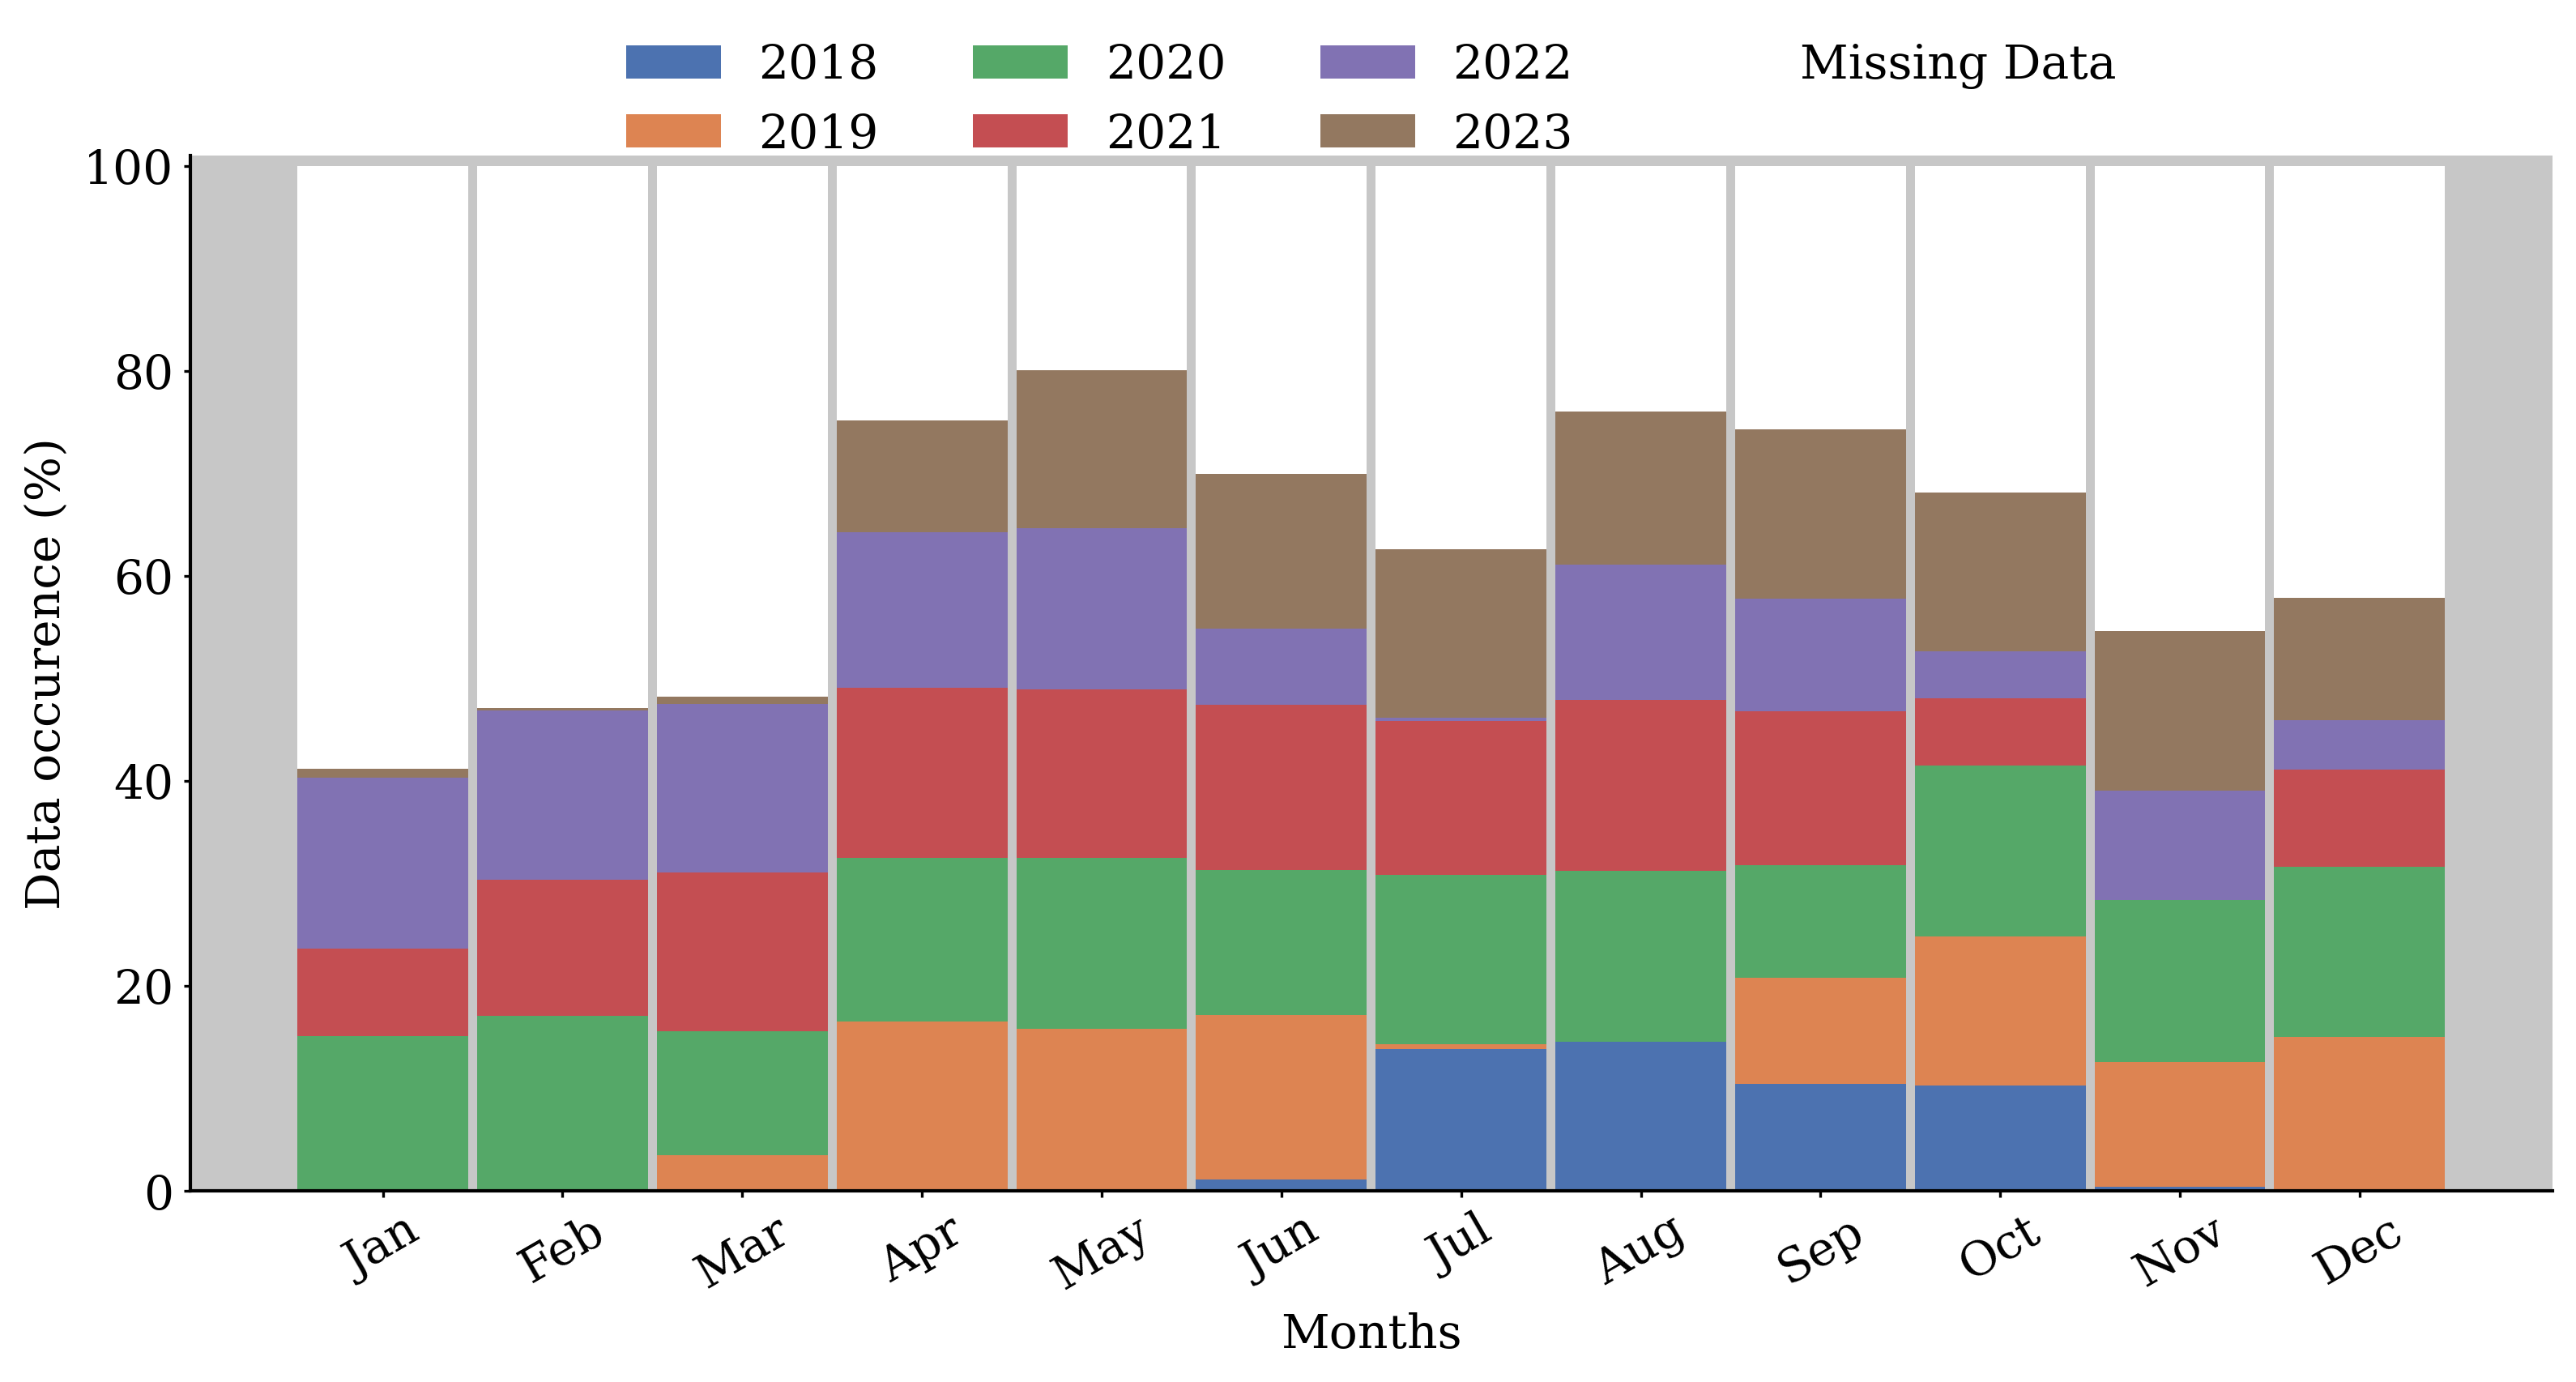
\includegraphics[width=.8\textwidth]{../../phd_clouds/figures/new_method_separated_monthly_data_occurence}
	\caption{High level post-processed data availability per month at the AGORA ACTRIS CCRES station. This dataset represents more than half a decade of synergic ground-based measurements at this station. Each color represents the data availability for different years.}
	\label{fig:data_availability}
\end{figure}

\subsubsection{Data processing}\label{sec:cloudnet_products}

Instrument datasets are processed by Cloudnet processing chain \citep{j.a.ContinuousEvaluationCloud2007} as follows:
\begin{enumerate}
	\item Set a common grid with a temporal resolution of 30\,s and spatial resolution according to the radar (see table \ref{tab:info_instrument}), respectively. It should be noted that this Cloudnet grid difficulties the monthly profiling on cloud statistics. Hence, another regrinding interpolating onto a height resolution of 20\,m is applied in the microphysics analysis.
	
	\item Corrections: this includes two-way gas and liquid reflectivity attenuation, error estimation, and quality flag assignment. High-frequency radars experience significant attenuation from gas and liquid droplets, necessitating signal correction. This issue is particularly pronounced during heavy rain events, where liquid layers on radome sheets can cause an attenuation of 14 dB \cite{hoganAbsoluteCalibration942003}.
	
	\item Cloud boundaries determination: lidar attenuated backscatter coefficient ($\beta$), and radar reflectivity are used. The first is sensitive to small liquid droplets present in cloud bases, as the second are able to penetrate clouds and detect their tops.
	
	\item Target classification product: This product classifies atmospheric particles into different categories by assigning an integer ranging from 0 to 10 at each pixel in the Cloudnet processed grid. Categorizes are as follows: Clear sky (0), Droplets (1), Drizzle or rain (2), Drizzle \& droplets (3), Ice (4), Ice \& droplets (5), Melting ice (6), Melting \& droplets (7), Aerosol (8), Insects (9), Aerosol \& insect (10). These targets were determined through radar and lidar variables in combination with thermodynamic profiles from the ECMWF model. In particular, wet bulb temperature (T$_w$) profiles are used to determine the 0$^{\circ}$C isotherm and establish warm and cold regions to identify liquid and ice hydrometeors. 
	
	\item Liquid layers respect a threshold of T < -40 $^{\circ}$C, since it is not possible to keep water in liquid phase below that temperature. Moreover, liquid droplets assigned as falling were classified as drizzle or rain droplets, where falling is attributed through radar echoes analysis once particle boundaries were already determined. Therefore, falling cold particles were just classified as ice, without distinguishing ice from precipitating ice.
	
	\item Melting layers were identified at the height of maximum wet bulb temperature divergence. Pixels with divergence surpassing 0.0075 s$^{-1}$ within 150 m of height deviation were also classified as "melting". Furthermore, more than one class of particle can be settled in the same pixel, allowing the identification of mixed phase hydrometeors, like ice coexisting with supercooled liquid droplets and melting ice particles coexisting with cloud liquid droplets. A more detailed description of particle apportionment of Cloudnet algorithm can be found on \citet{hoganFacilitatingCloudRadar}. 
	
	\item The liquid water content (LWC) retrieval assumes a log-normal distribution for warm cloud droplets lifting adiabatically from its base. Its relation depends on atmospheric temperature (T) and pressure (P). This method incurs a relative uncertainty of 15\% as shown by \cite{a.s.frischCloudRadarMicrowave1998}. At our station, T and P values utilized by the LWC retrieval are provided by the European Centre for Medium-Range Weather Forecasts (ECMWF). The retrieval equation is applied exclusively to liquid pixels within cloud boundaries, which are determined by Doppler radar reflectivity (Z) and ceilometer-lidar attenuated backscatter coefficient. The liquid pixels, as ice, insect and aerosol pixels are given by the cloudnet target classification product \citep{hoganFacilitatingCloudRadar}. Additionally, LWC values are scaled to align with the Liquid Water Path (LWP) derived from the microwave radiometer. The liquid cloud droplet effective radius ($r_{liq}$) is retrieved by assuming a log-normal size distribution for warm cloud droplets. This method is insensitive to droplet number concentration and the logarithmic spread of the distribution \citep{s.frischRetrievalStratusCloud2002}. Consequently, its primary source of uncertainty is the reflectivity factor error, resulting in a relative error of 15\% for $r_{liq}$ retrievals. This relationship is applied exclusively to liquid pixels, where necessary input data, assumptions, relative errors and the studies from which these products are sourced are indicated in Table \ref{tab:microphys}).
	
	\item The ice water content (IWC) retrieval employs an empirical equation as determined by \cite{robinj.hoganRetrievalIceWater2006}, known as the Z-IWC-T relation, which depends on radar reflectivity and temperature. Compared to other microphysical variables, IWC retrievals has the largest relative uncertainties. For the W-band, the relative error is +55\% to -35\% for temperatures within the range of -20$^{\circ}$C to -10$^{\circ}$C, and +90\% to -47\% for T < -40$^{\circ}$C. While temperature is a significant parameter in IWC error estimation, \cite{pablosaavedragarfiasAsymmetriesCloudMicrophysical2023} demonstrated that the primary source of uncertainty is the reflectivity factor error. A typical reflectivity error of 3\% can result in a 12\% error in the ice water path (IWP), which is the integration of IWC over the atmospheric column. Therefore, errors in IWC can be relatively large. The Z-IWC-T relation is applied only to ice pixels within cloud boundaries. Next, the ice cloud particle effective radius ($r_{ice}$) is obtained following \cite{juliendelanoeCharacterizationIceCloud2007}, who assumed the same empirical relation for IWC and the visible extinction coefficient ($\alpha$) derived by \cite{robinj.hoganRetrievalIceWater2006}. This approach, termed the Z-T relation, depends on both T and Z, and has aThis approach, termed the Z-T relation, depends on both T and Z, and has a relative uncertainty of 50\% of $r_{ice}$ \citep{hannesgriescheApplicationShipborneRemote2020}. In general, these high relative errors emphasize how challenging it is to retrieve ice properties accurately (see Table \ref{tab:microphys})
\end{enumerate}

% Please add the following required packages to your document preamble:
% \usepackage{booktabs}
% \usepackage{multirow}
\begin{table}[H]
	\caption{Cloudnet microphysics products used in this study, their inputs and assumptions}
	\begin{tabular}{@{}llll@{}}
		\toprule
		\textbf{Cloudnet products}                  & \textbf{Input role}                              & \textbf{$\sigma_{re}$/$r_{e}$} & \textbf{References}                                                                \\ \midrule
		\multirow{3}{*}{Liquid water content (LWC)} & Z and $\beta$: cloud base and top identification & \multirow{3}{*}{15\%}          & \multirow{3}{*}{Frisch et al. (1998)}                                              \\
		& T, P, assuming an adiabatic lifting          &                                &                                                                                    \\
		& MWR or CDR LWP to scale LWC                      &                                &                                                                                    \\
		Ice water content (IWC)                     & Z and T profiles                        & -35\% to 90\%                        & \begin{tabular}[c]{@{}l@{}} \cite{robinj.hoganRetrievalIceWater2006} \\ \cite{juliendelanoeCharacterizationIceCloud2007}\end{tabular} \\
		Droplet effective radius ($r_{liq}$)       & Z, and N and $\sigma$ of lognormal PSD           & 15\%                           & \cite{s.frischRetrievalStratusCloud2002}                                                               \\
		Ice effective radius ($r_{ice}$)          & Z and T                                & 50\%                        & \cite{hannesgriescheApplicationShipborneRemote2020} \\ \bottomrule
	\end{tabular}
	\label{tab:microphys}
\end{table}

\section{Methodology}\label{sec:classification_algorithm}

\subsection{Cluster classification method}\label{sec:new_method}

The cluster-based algorithm is developed in order to homogenize cloud clusters in time. Different from the profile-based method, this method avoids high correlation between distinct cloud categories (e.g. ice and mixed-phase). In both cases, the Cloudnet target classification product is used as a basis for cloud typing. This product provides the hydrometeor type information for each profile. Thus, the pixels classified as hydrometeors, such as Droplets, Ice and Drizzle \& Droplets are used to classify clouds. In the case of the profile-based method, \cite{buhlMeasuringIceLiquidwater2016} already adapted it for only mixed phase clouds, selecting only cases with more than 15 min of coherent cloud profiles (with similar cloud profiling within 300 s). Nevertheless, by adding new criterias to identify liquid and ice clouds, this method can classify segments of one cloud in different categories, depending on the time threshold. Hence, we introduce a new approach that does not classify cloud profiles neither segments, but cloud clusters.

Prior to the use of the target classification product, a preprocessing of the data was required. It has been observed that for some specific cases, misclassification of some pixels may occur. Figure \ref{fig:cloudnet_misclassification} illustrates a thinner and lower precipitable ice cloud present between 08:00 and 20:00. However, there is no evidence of clouds in the attenuated backscatter and the radar reflectivity. These misclassifications stem from an inaccurate representation of the temperature profile by the models in the region of Granada, affecting the target classification algorithm, and subsequently, the cloud classification performed in this study. To mitigate these issues and prevent misinterpretation of future cloud statistics, we established a filter to detect and remove these cases. Basically, all these clouds which were identified with mean cloud base below 4 km (above mean sea level) and average cloud thickness below 700 meters were reclassified as noise. These values were determined empirically by studying many cases separately. 

\begin{figure}[H]
	\centering
	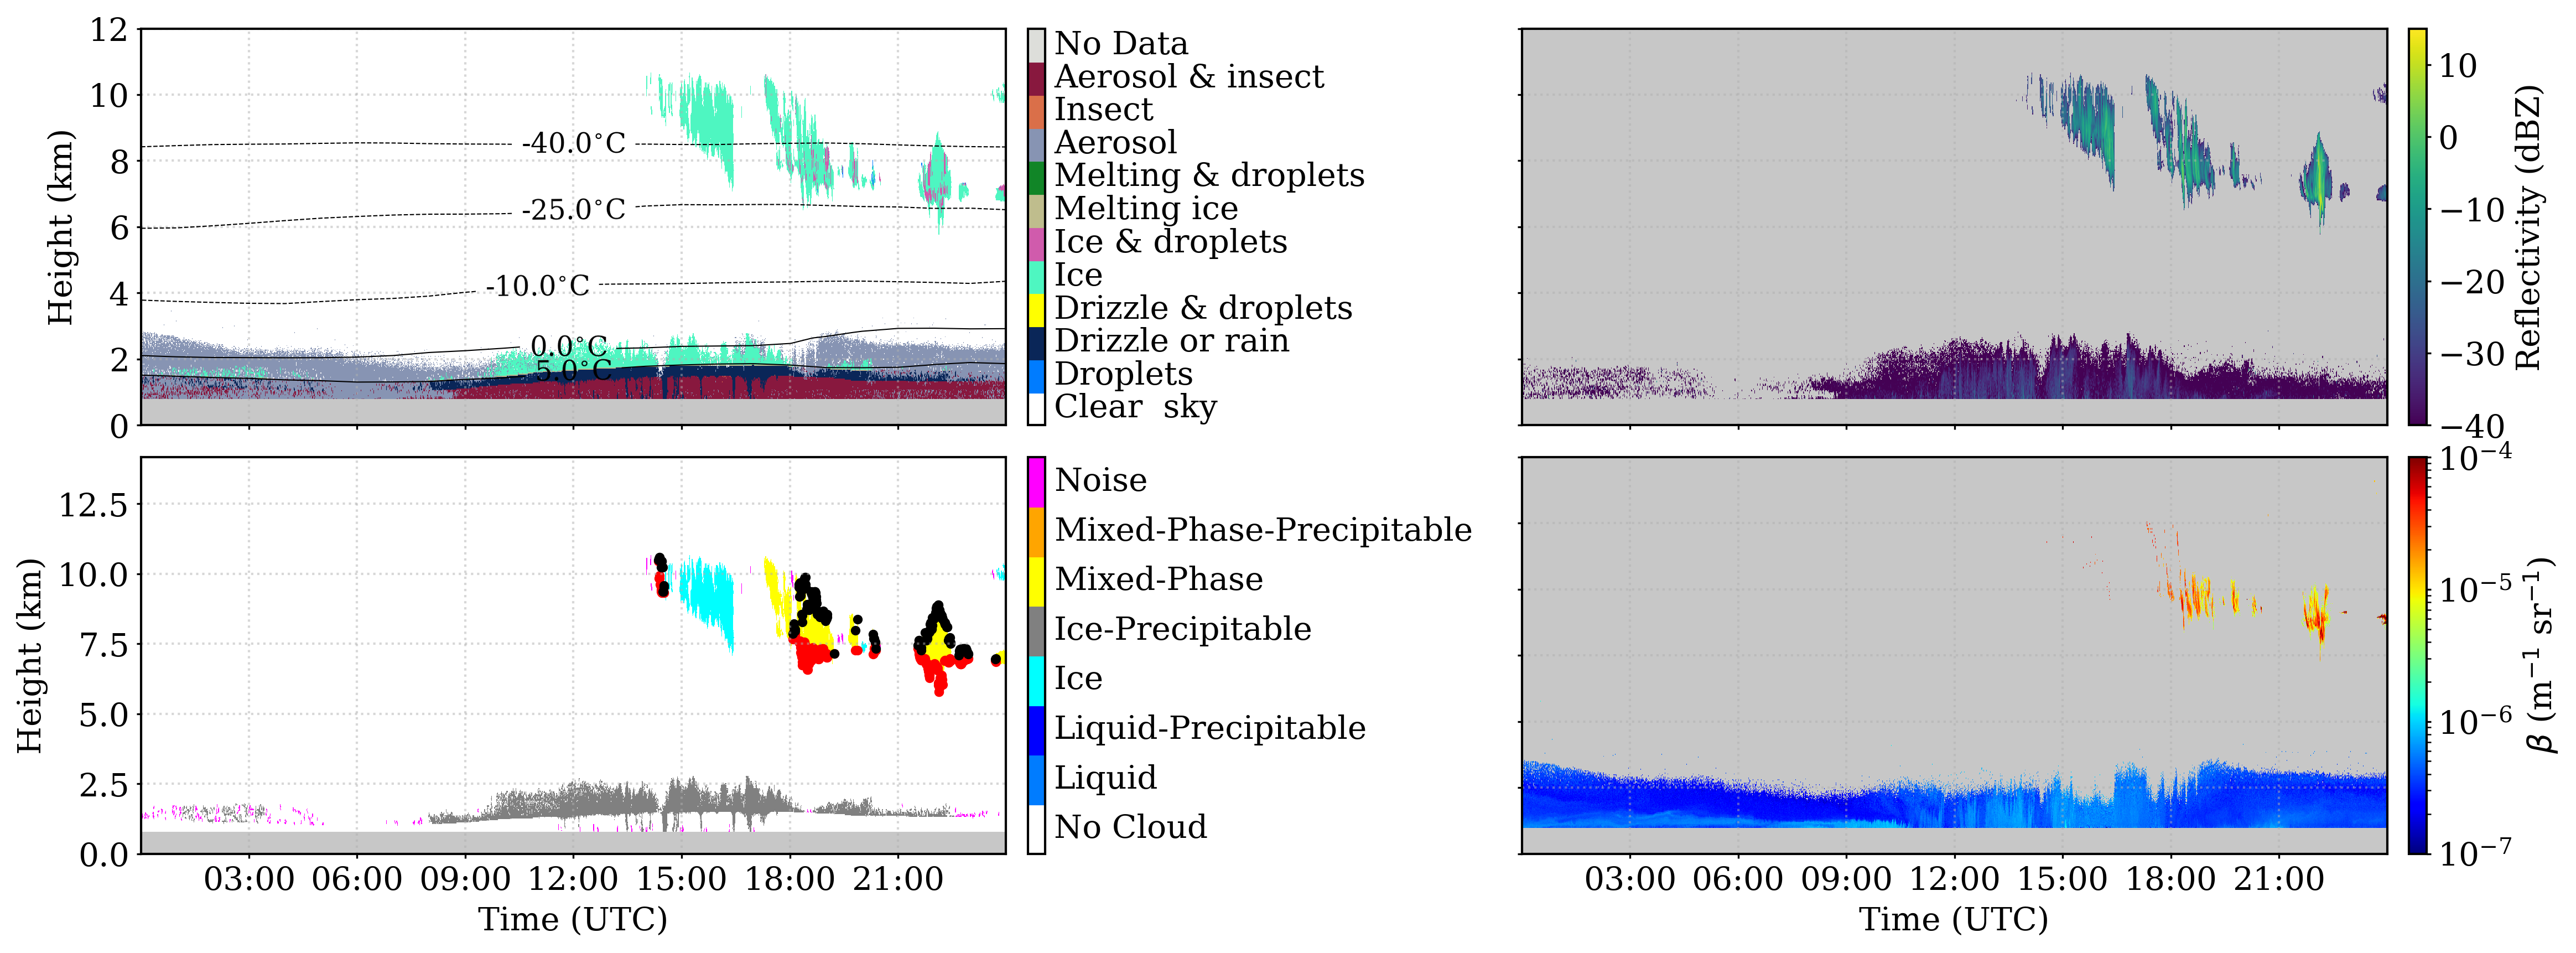
\includegraphics[width=\textwidth]{../../phd_clouds/figures/20210418_cloudnet_misclassification}
	\caption{A case study of Cloudnet hydrometeor misclassification. (a) Target classification product; (b) Radar reflectivity factor from Doppler cloud radar; (c) Attenuated backscattering coefficient from ceilometer. No evidence of clouds in the ABL can be identified by the instruments.}
	\label{fig:cloudnet_misclassification}
\end{figure}

Once the data are curated, the different cloud types are identified. Recent studies employed a cloud classification algorithm by profile with the aim of classify clouds
\citep{razvanpirloagaGroundBasedMeasurementsCloud2022, tatiananomokonovaStatisticsCloudsTheir2019, stefankneifelMultiyearCloudPrecipitation2021} and analyze their statistics. However, this algorithm admits different cloud typing inside the same cloud as a whole, assigning similar physical properties for different clouds. In the appendix \ref{sec:old_method}, we describe this algorithm, adapting the criteria used by \cite{razvanpirloagaGroundBasedMeasurementsCloud2022, tatiananomokonovaStatisticsCloudsTheir2019}.  
In this study we propose a new methodology to overcome these inaccuracies. We define a cloud as a group of at least 100 pixels identified by Cloudnet as droplet, drizzle (see Figure 3). To do so, a cloud mask is generated from the CLOUDNET target classification. Cloud pixels separated only by two pixels in any direction (analogous to 1 min, and 20 - 50 m of height) are considered part of the same cloud. This is achieved using a pixel dilation and contraction technique \citep{doughertyMathematicalMorphologyImage2018}, which expands and contracts the cloud shapes (see Appendix \ref{sec:dilation} for an explanation of the method). Once the cloud pixels are grouped, each cloud must have more than 100 pixels to be considered (without considering rain such as Drizzle or Rain pixels). Otherwise, it is deemed as an unknown type (likely noise). In order to illustrate this method, the left panel of Figure \ref{fig:cluster_identification} shows cloud clusters of different colors during an entire day (on 11 February 2021). The regions identified as clouds are marked by the black dashed lines in the right panel of the same figure, where clusters that are very close will merge to form one cloud. Also, small and isolated groups with less than 100 pixels are indicated by the red dashed lines

\begin{figure}[H]
	\centering
	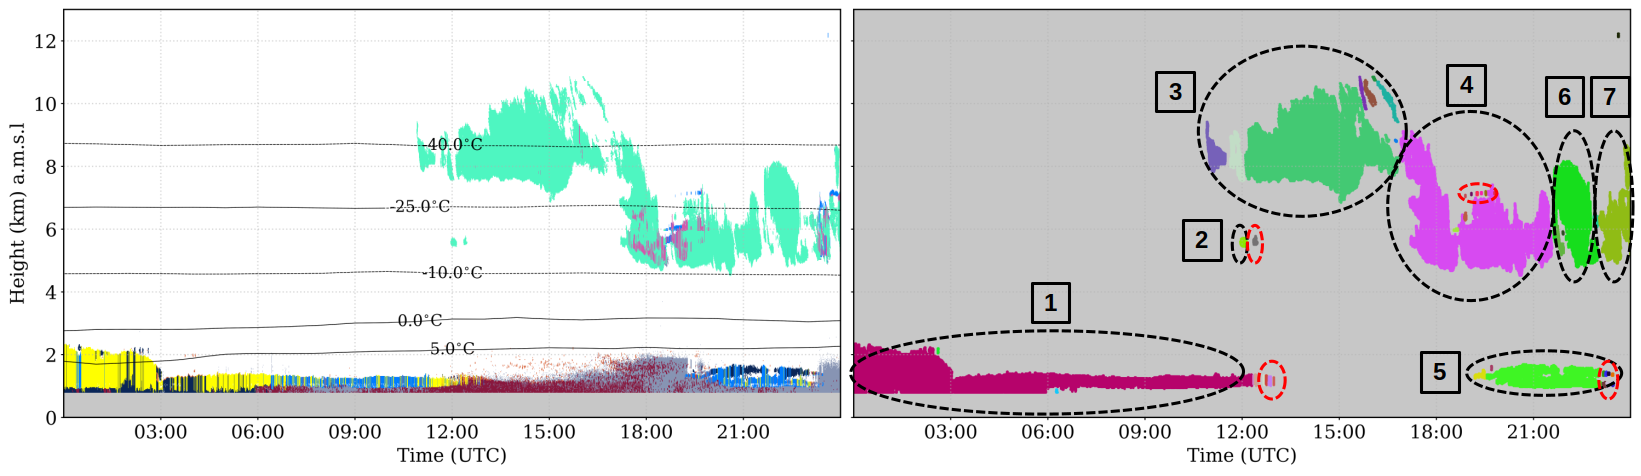
\includegraphics[width=.85\textwidth]{../../phd_clouds/figures/scheme_cloud_identification}
	\caption{Cloud cluster identification by Cloudnet target classification on 11 February 2021. (a) All hydrometeor clusters identified at different colors; (b) Cloud clusters identified in black dashed lines and noise by red dashed red}
	\label{fig:cluster_identification}
\end{figure}

Then, clouds are classified in six types: liquid, ice, mixed-phase, precipitating liquid, precipitating ice, and precipitating mixed-phase. To do so, the hydrometeor type percentages are calculated for each cloud, (shown in figure \ref{fig:classificationby_group_scheme}). A cloud is classified as liquid cloud (Liquid criteria) it comprises more than 70\% of Droplets and Drizzle plus Droplets. Then, it is further classified as a precipitating liquid cloud (Rainy criteria) if it contains at least 10 connected rain pixels, Similarly, a cloud is classified as an ice cloud (Ice criteria) if the previous verification is not satisfied and if  this group contains more than 90\% of ice or less than 10\% of Droplets plus Ice \& droplets. The same rain verification as in the liquid case is made to classify this group as a pure ice cloud or a precipitating ice cloud. Otherwise, clouds are classified as mixed-phase or precipitating mixed-phase through the same rain verification as in the other clouds.
In relation to precipitating ice and precipitating mixed-phase clouds, an extensive analysis of individual case studies revealed that Drizzle \& droplets only appear below the melting layer together with Drizzle \& rain droplets. Therefore, to avoid an underestimation of cloud base height due to drizzle, we removed these pixels for these clouds since they are probably rain.

\begin{figure}[H]
	\centering
	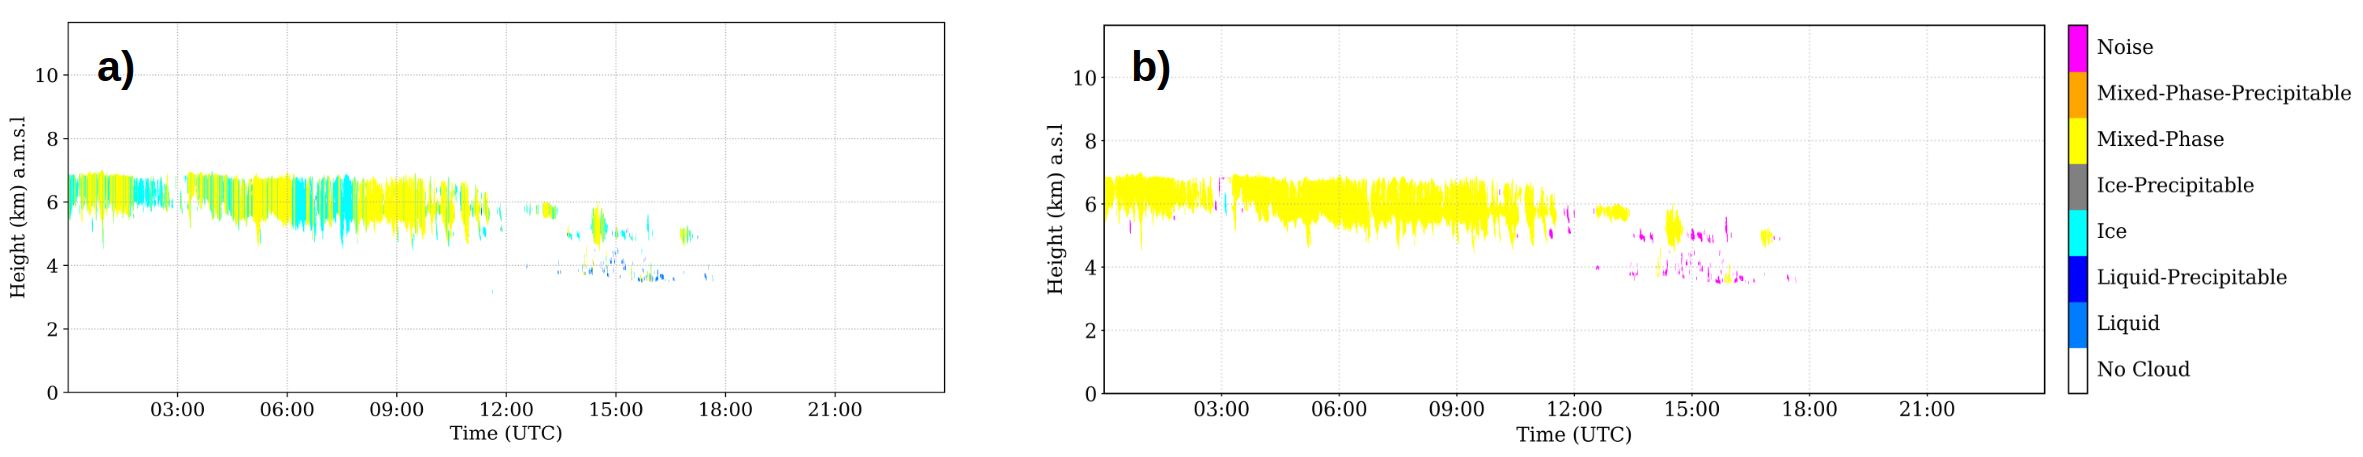
\includegraphics[width=.9\textwidth]{../../phd_clouds/figures/scheme_cloud_classification}
	\caption{Scheme of the cloud classification algorithm by hydrometeor grouping}
	\label{fig:classificationby_group_scheme}
\end{figure}

After the cloud classification, each cloud is then classified as single or multi-layer over time. Initially, time intervals where clouds overlap are identified. Overleaped pieces of clouds are classified as multi-layer, whereas non-overlapping pieces in principle are classified as single layer.We then analyzed cloud profiles for each cloud individually, acknowledging that a cloud can exhibit multiple layers with itself. If a cloud had a second layer separated by only one pixel at some time interval, that interval is identified as containing multi-layer. Otherwise, the clouds at that interval are classified as a single layer. 

In this study, only single layer clouds are analyzed. For the single layer case, cloud properties are calculated as follows: the cloud base and top height are determined by the first and last height pixels within the cloud layer, respectively. Cloud thickness is obtained by the difference between cloud base and top height pixels. 

\subsection{Cloud typing assessment}\label{sec:daily_cycle}

An evaluation of the classification algorithm presented in this study against the method used in the literature is conducted in order to evaluate its applicability for further analysis. Here, we aim to provide insights into the correlation on cloud statistics between different cloud categories generated by these two methods. In this framework, Figure \ref{fig:cloud_classification_comparison} shows a case study on 6 May of 2023 in Granada comparing profile-based cloud classification and cluster classification for a mixed phase cloud, where red and black dots represent the cloud base and top, respectively. As expected, the profile-based classification on the right panel leads to the fragmentation of a single cloud into different types. In this case, the same cloud is being classified as ice and mixed-phase by time. On the other hand, in the left panel, the new classification method preserves the homogeneity of the cloud and classifies it as mixed-phase cloud, resulting in a more realistic classification.

\begin{figure}[h]
	\centering
	\begin{subfigure}{0.48\textwidth}
		\centering
		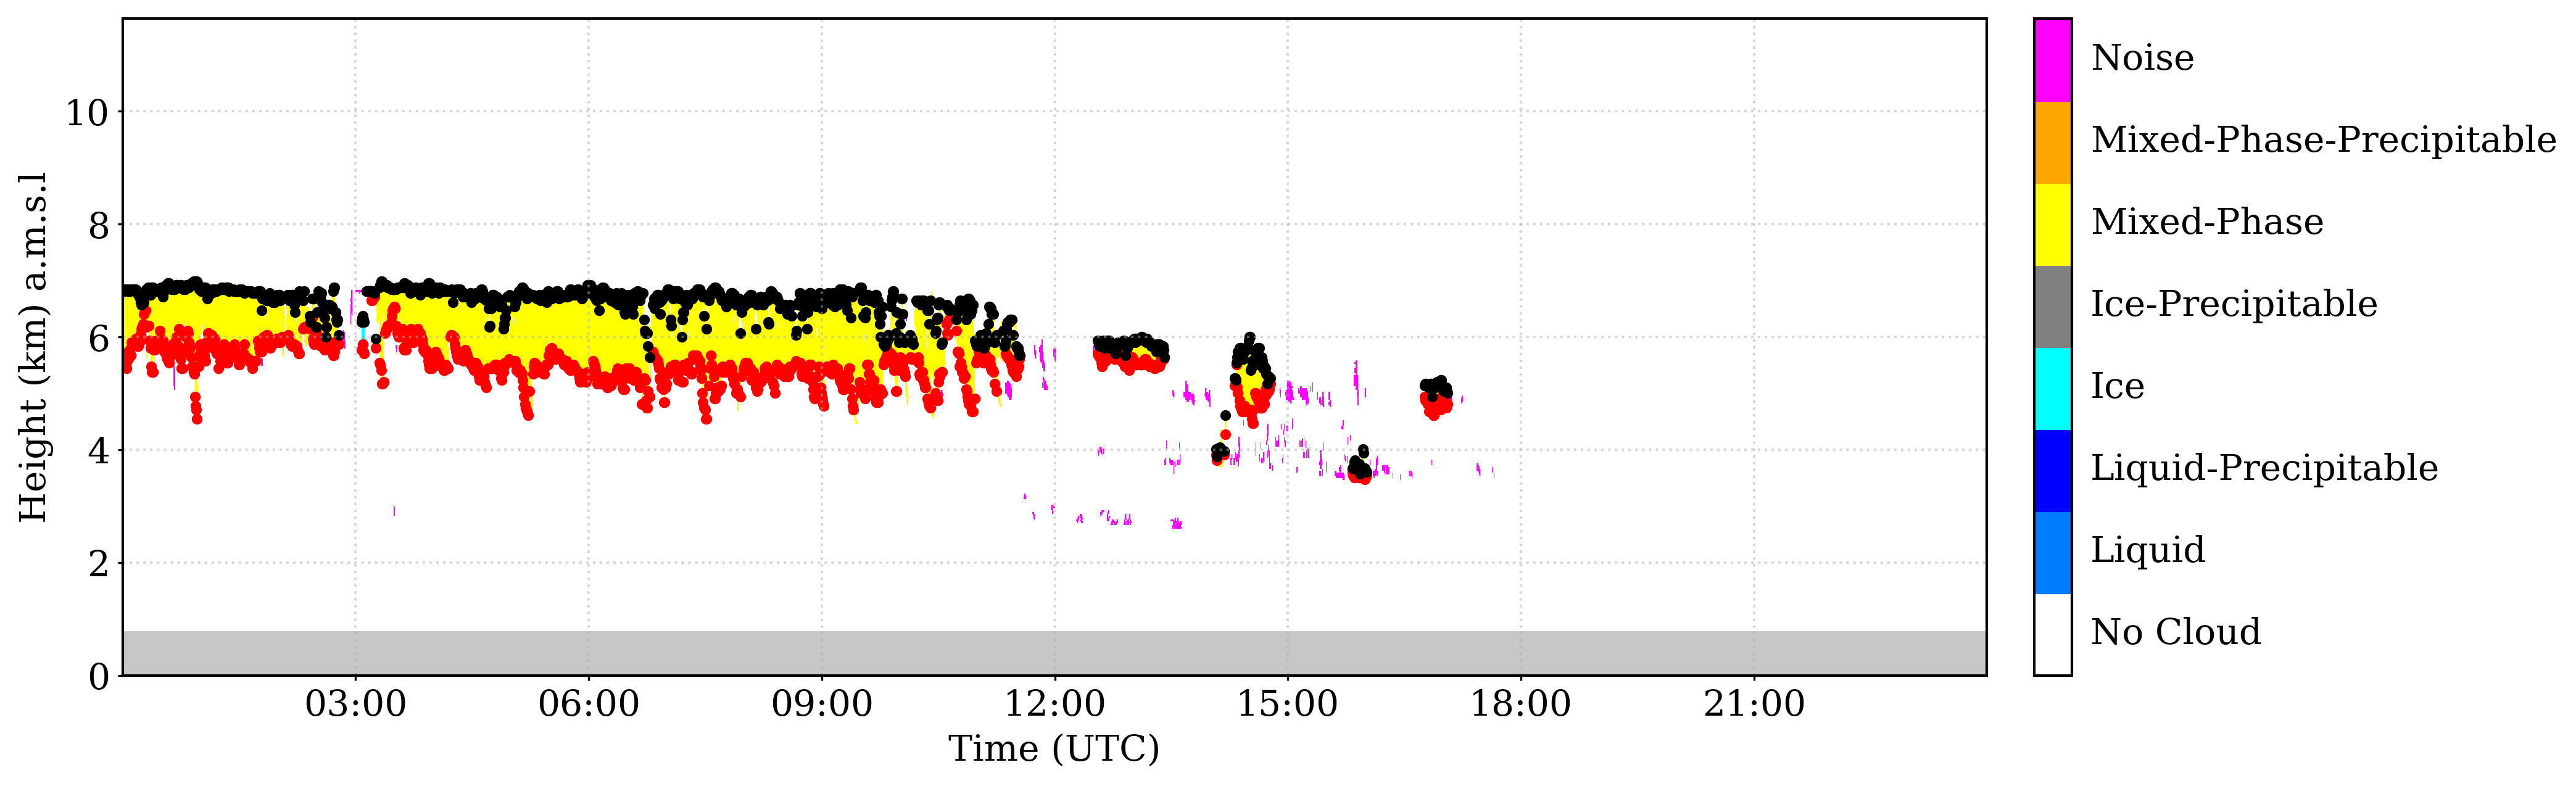
\includegraphics[width=\textwidth]{../../phd_clouds/figures/20230506_cloud_classification_new_method}
		\caption{Cloud classification using the new method.}
		\label{fig:new_method}
	\end{subfigure}
	\hfill
	\begin{subfigure}{0.48\textwidth}
		\centering
		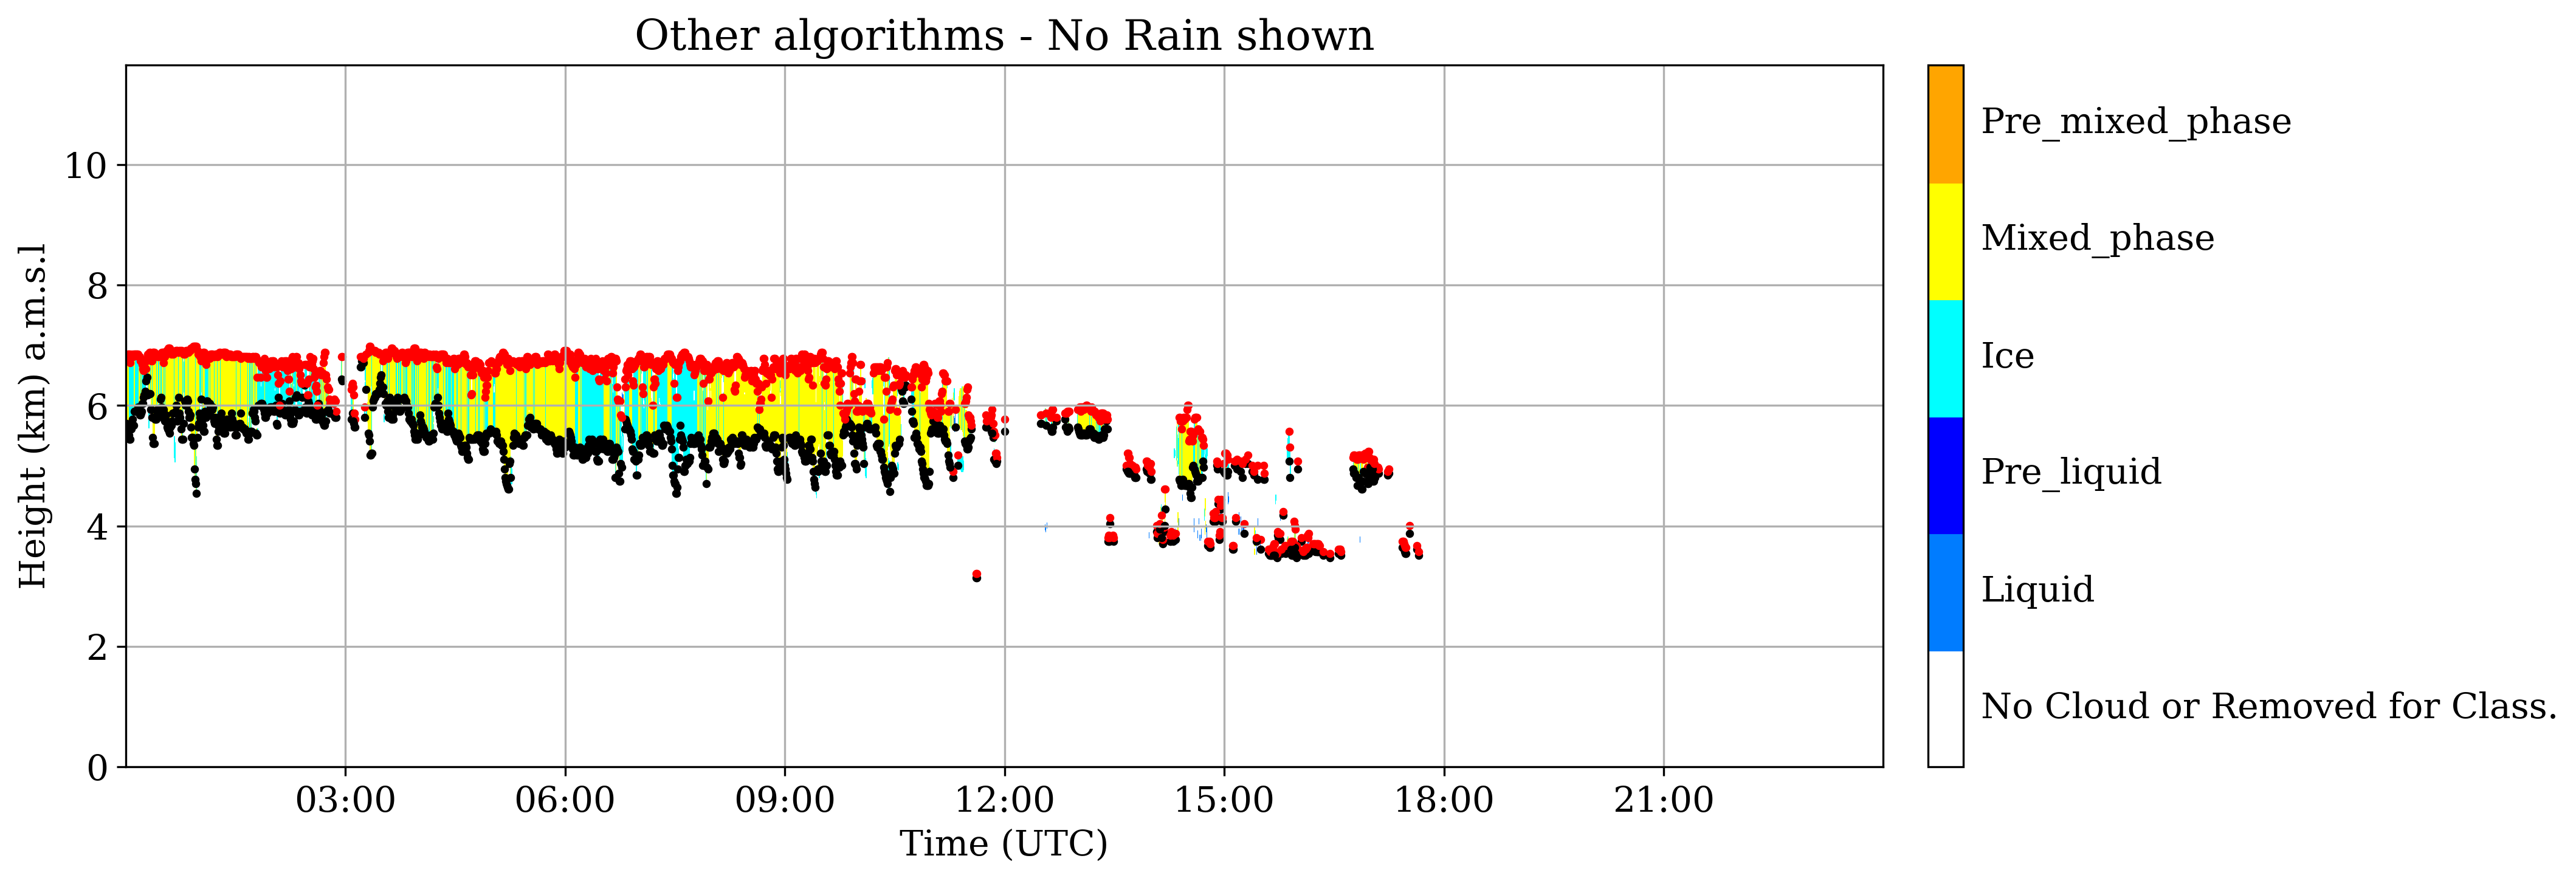
\includegraphics[width=\textwidth]{../../phd_clouds/figures/20230506_cloud_classification_old_method}
		\caption{Cloud classification using the old method.}
		\label{fig:old_method}
	\end{subfigure}
	\caption{Temporary figure (needs target classification). Comparison of cloud classification methods. The left panel illustrates the new method, which preserves cloud homogeneity and provides a more realistic classification. The right panel shows the old method used in recent studies, where cloud classification is time-based.}
	\label{fig:cloud_classification_comparison}
\end{figure}

As a consequence, the profile-based method of cloud classification can generate high correlations between cloud categories in terms of frequency of occurrence and cloud properties. Regarding cloud occurrence, the right panel of Figure~\ref{fig:cloud_classification_comparison} suggests that both ice and mixed phase clouds will have similar daily cloud occurrence and average cloud base. However, this is occurring because of the classification method, which could further affect cloud statistics.

Therefore, in order to quantify the correlation between cloud categories generated by these two classification algorithms, we calculate the daily cloud occurrence to assess the correlation between cloud types. Figure \ref{fig:pearson_correlation} shows the pearson correlation coefficients of daily cloud occurrence between cloud types for the cluster classification on the left, and for the classification by profile on the right. As it can be seen, the new proposed method demonstrates generally weaker correlations among cloud types, with most values clustering around zero. For example, the highest correlations observed were 0.19 between Liquid and Liquid-Precipitable clouds and 0.17 between Liquid and Mixed-Phase-Precipitable clouds, indicating relatively weak relationships. Additionally, some negligible negative correlations were observed, e.g. between Ice and Mixed-Phase-Precipitable clouds (-0.1). This suggests that the new method may provide a clearer distinction between cloud types, which is advantageous for analyses requiring precise classification. In contrast, the profile-based classification exhibited stronger and more pronounced correlations. Notably, the correlation between Ice and Mixed-Phase clouds was 0.4, and between Liquid and precipitating liquid clouds was 0.32, highlighting significant interdependencies between these cloud types. These relatively higher correlations are a consequence of the classification scheme defined in this method, which allows tagging multiple cloud types inside the same cloud domain. As a result, the comparison indicates that the new method, with its generally weaker correlations, may be better suited for distinguishing different cloud types. These findings underscore the importance of selecting an appropriate analytical method to study cloud properties between different cloud types.

\begin{figure}[H]
	\centering
	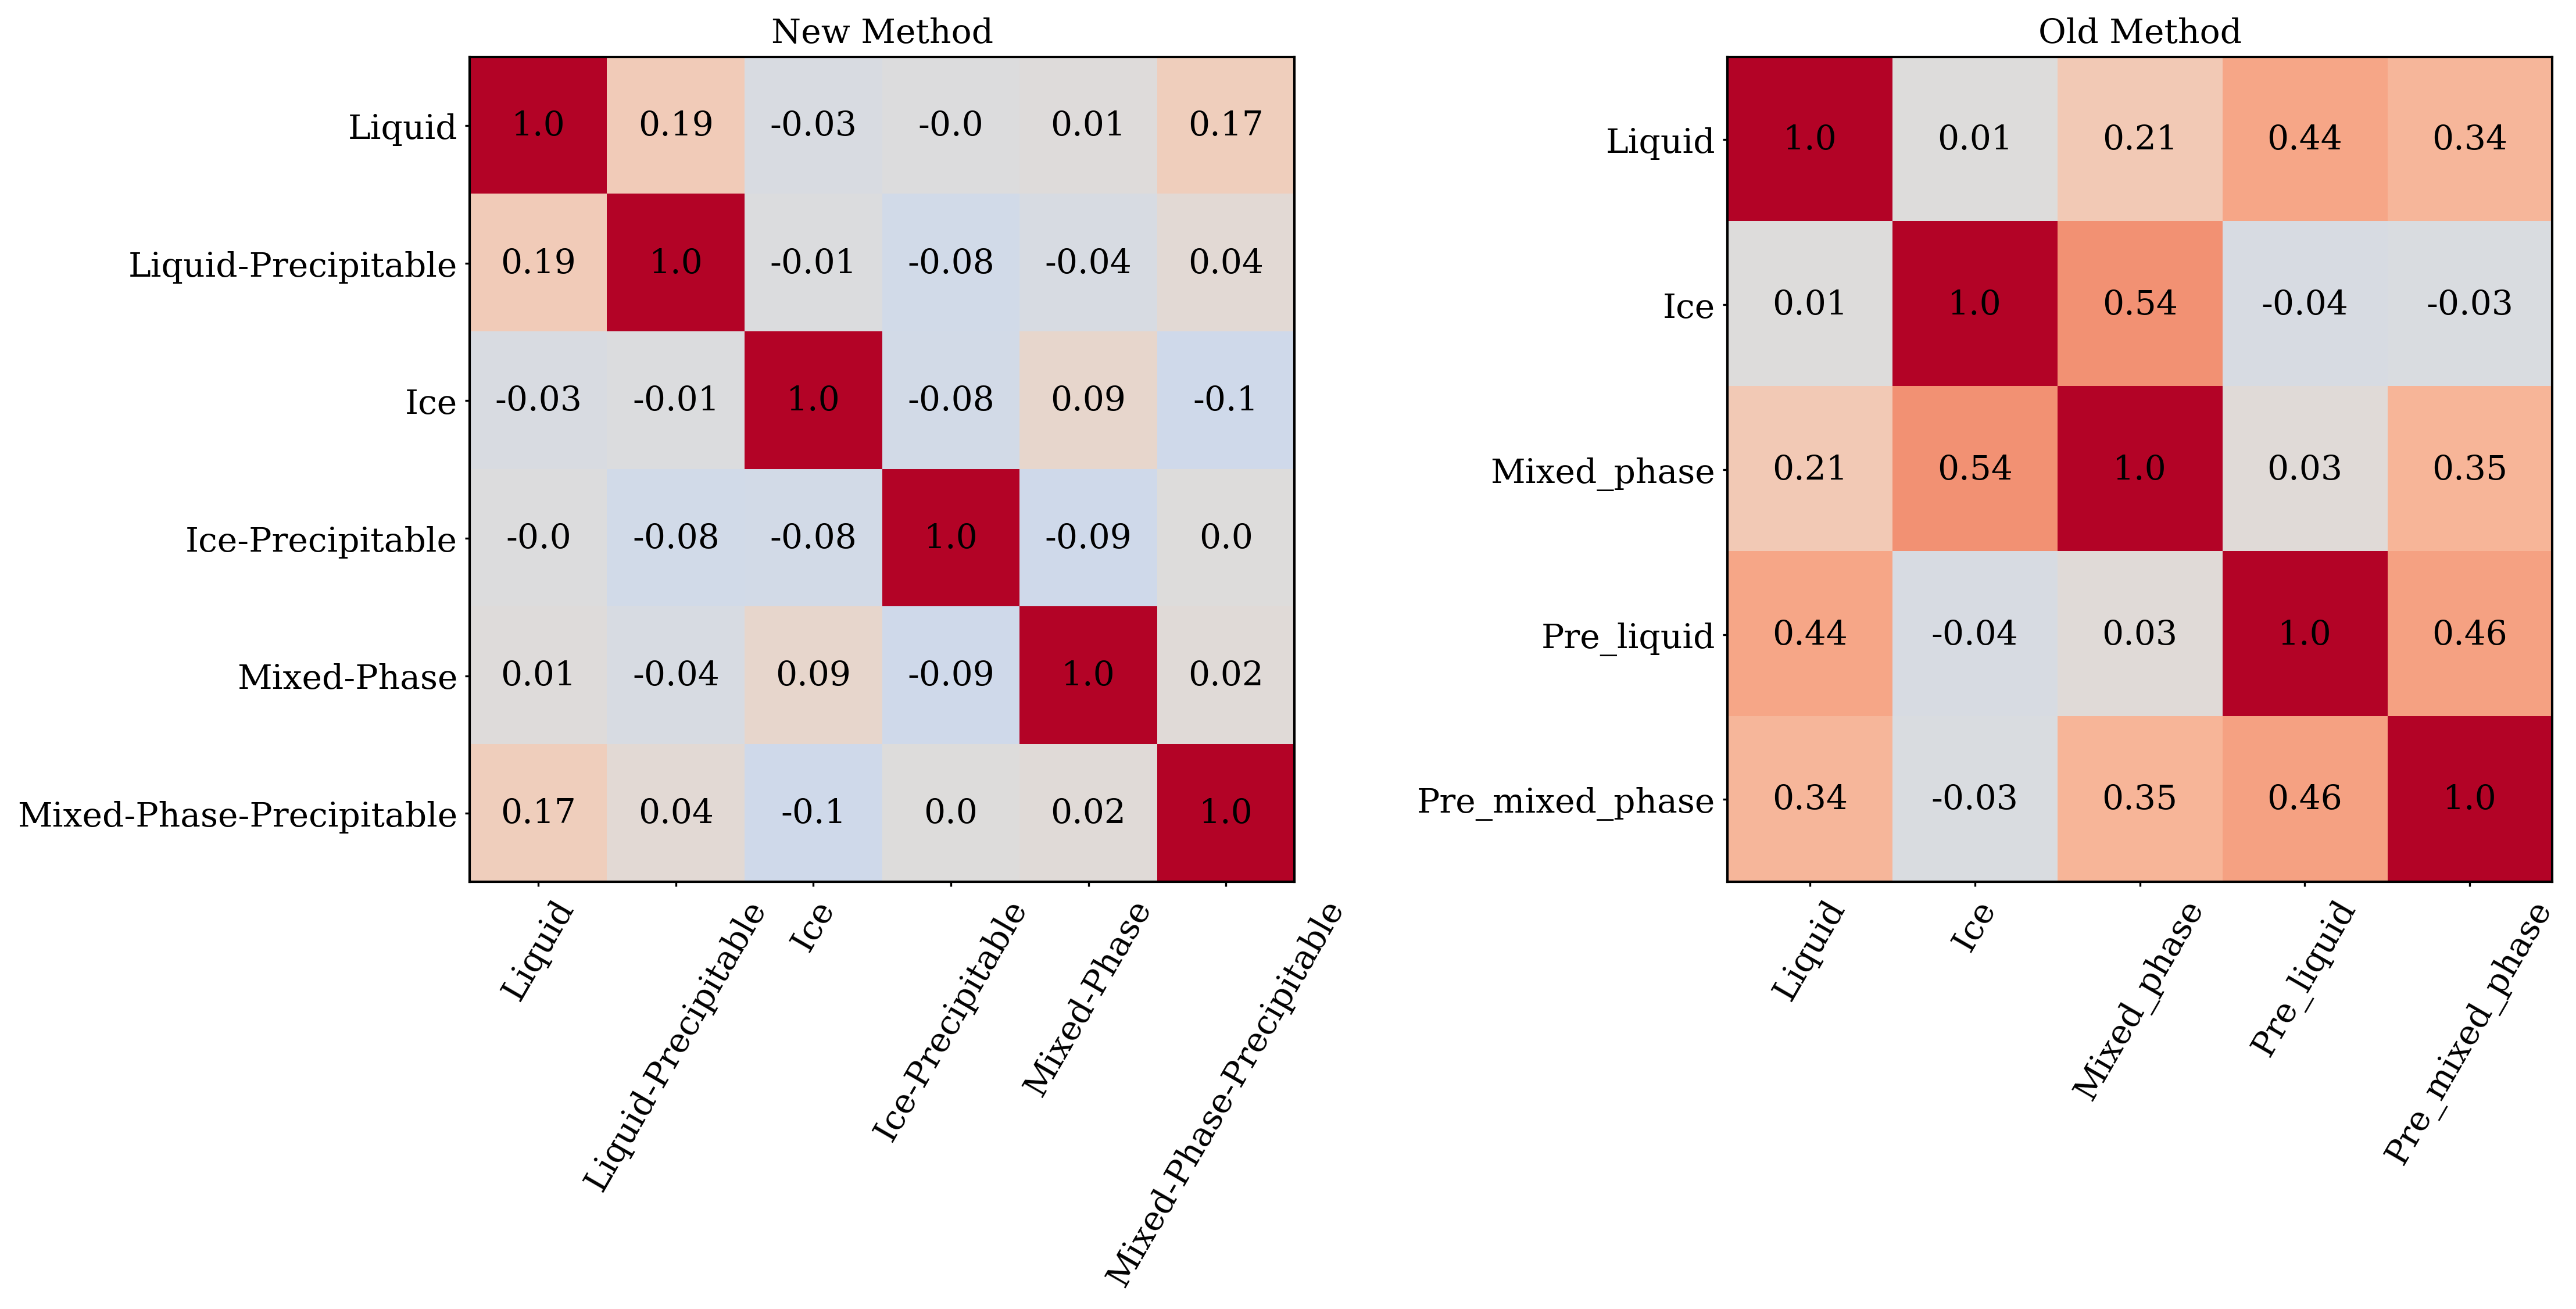
\includegraphics[width=.8\textwidth]{../../phd_clouds/figures/cloud_freq_methods_comparison_correlation_coefficient}
	\caption{The Pearson correlation matrix of daily cloud occurrence among different cloud types is shown in the top panel. The correlations for cluster-based methods are on the left and the profile-based correlation is on the right. Below each correlation matrix, the corresponding comparison of IWC between ice and mixed phase is shown.}
	\label{fig:pearson_correlation}
\end{figure}

Regarding the correlation in cloud properties, we computed the daily average of IWP for ice and mixed-phase clouds for the two classification methods. The bottom panel of Figure \ref{fig:pearson_correlation} shows the IWP of mixed phase clouds in function of the IWP of ice clouds. The R factor is the Pearson correlation coefficient between the IWP of these two cloud types. This coefficient is quite higher for the profile-based method, showing a correlation of 0.7. On the other hand, the cluster method exhibited only 0.24, with no apparent correlation. In addition, the correlation seems to be not monthly dependent as there is no clear separation by month. It is worthy to note that this section is not focused on the analysis of IWP, this will be done in section \ref{sec:cloud_microphys}. Instead of this, here we focused on the influence of the classification algorithm on cloud properties analysis. Following, the observations suggest that statistics on cloud properties can be highly influenced by the profile-based classification. As a result, this method may lead to the misinterpretation of real cloud properties, raising the relevance of previous evaluation of cloud classification algorithms before doing statistics on cloud properties. In this light, the new approach shows a promising classification method and will be employed in this study.




%\section{Results and discussion}
%\subsection{Annual variability and daily cycle of clouds}\label{sec:daily_cycle}

Since the cloud classification by hydrometers grouping showed a more comprehensive classification, this algorithm is employed in the following analysis. This section aims to analyze the inter-annual and daily cycle variability of cloud frequency of occurrence at the Granada station. In this framework, a first overview on cloud occurrence is given by the left panel of Figure \ref{fig:cloud_available}, which shows the monthly frequency of occurrence of different sky conditions, categorized into single-layer clouds, multi-layer clouds, clear sky, and noise (as explained in section \ref{sec:new_method}). The data reveal a distinct seasonal pattern in cloud cover and clear sky occurrences. Clear sky conditions (green line) are predominant all year long, being most frequent in the summer months, peaking in July and August (> 80\%), with a significant decline in spring, reaching the lowest point in March and April (40\%). This pattern indicates a higher prevalence of clear skies during the warmer months and increased cloudiness during the colder months. 
Single-layer clouds (blue line) exhibit a relatively weak seasonal pattern throughout the year, with a slight peak in spring (35\%) and a decrease in the summer months (10\%), suggesting a moderate variation in single-layer cloud occurrences. Multi-layer clouds (orange line) show a similar pattern, with a peak in March and April and a reduction during the summer, indicating a seasonal preference for multi-layer clouds in the spring, when there is more multi-layer than single-layer. The noise category (red line) maintains a weak seasonal pattern throughout the year, comparable with multilayer in later spring and summer. 
Overall, the data highlight clear seasonal variations in sky conditions, with clear skies dominating in summer and increased cloudiness, both single and multi-layer, in the cooler months. Since this station exhibits a quite low cloud occurrence, a need to handle multilayer clouds is revealed to fill gaps of cloud properties at regions such as the western Mediterranean. Particularly, these multi-layer are problematic due to inaccurate LWP partitioning, leading to a misclassification of liquid pixels inside clouds, as observed by \cite{tatiananomokonovaStatisticsCloudsTheir2019}. Therefore, the following analyses are focused only on single-layer clouds, seeing their physical properties can be retrieved more accurately.

\begin{figure}[H]
	\centering
	\begin{subfigure}{0.48\textwidth}
		\centering
		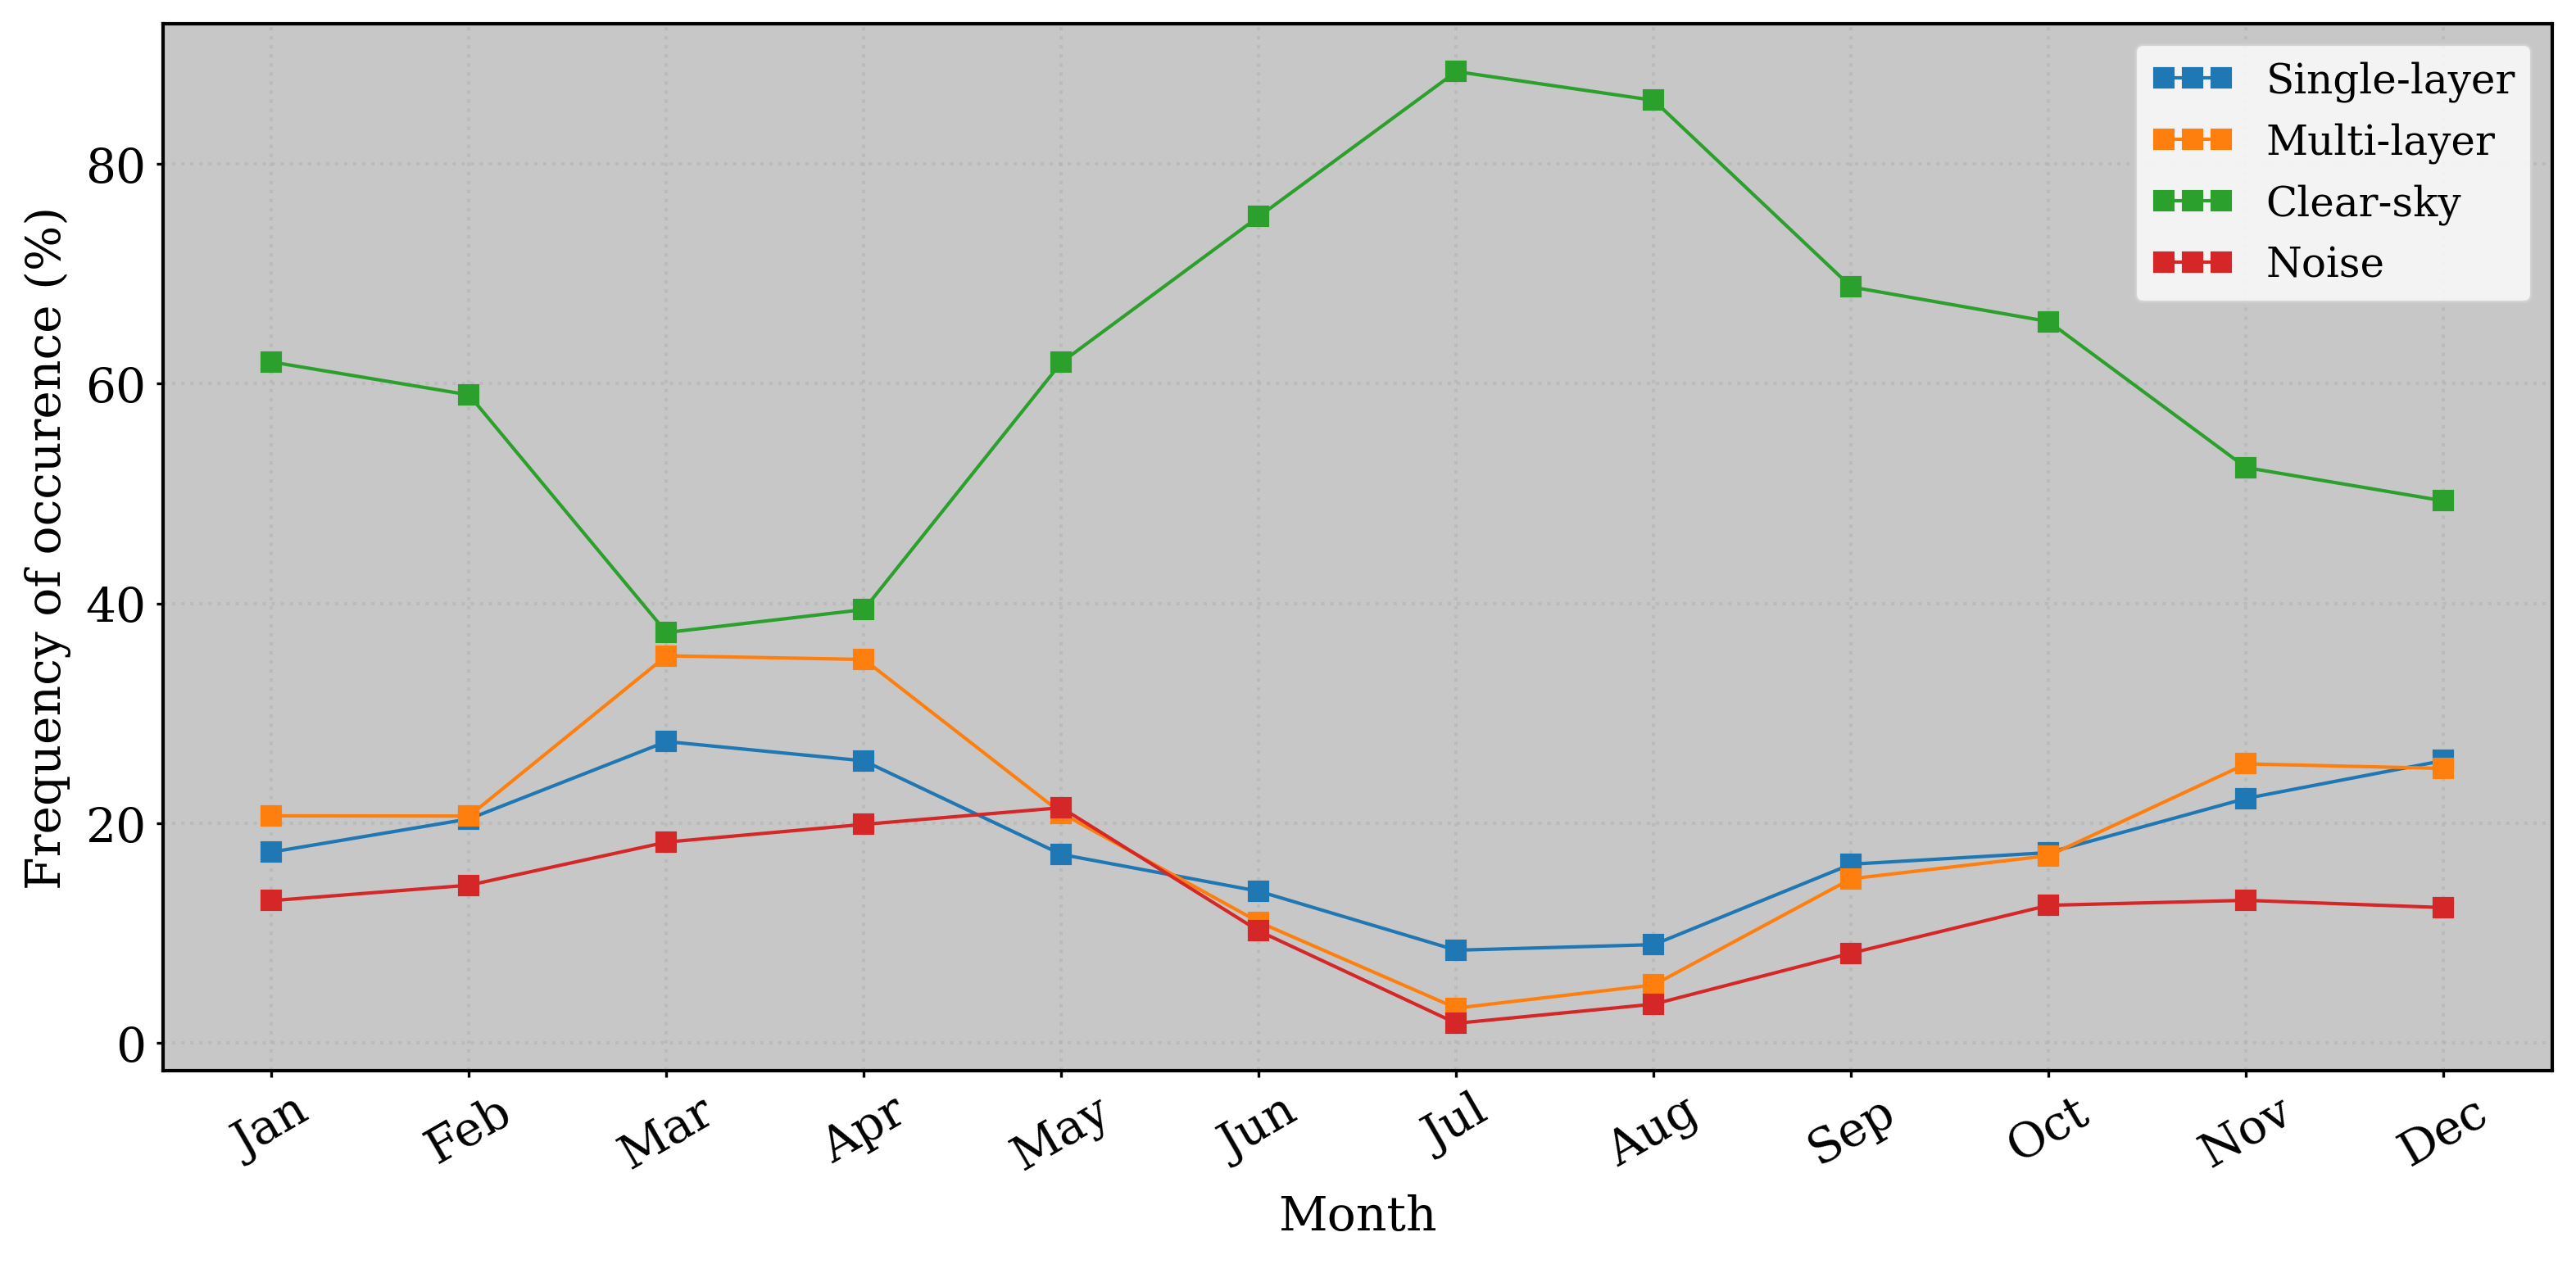
\includegraphics[width=\textwidth]{../../phd_clouds/figures/new_method_monthly_cloud_occurence.png}
		\caption{}
	\end{subfigure}
	\hfill
	\begin{subfigure}{0.48\textwidth}
		\centering
		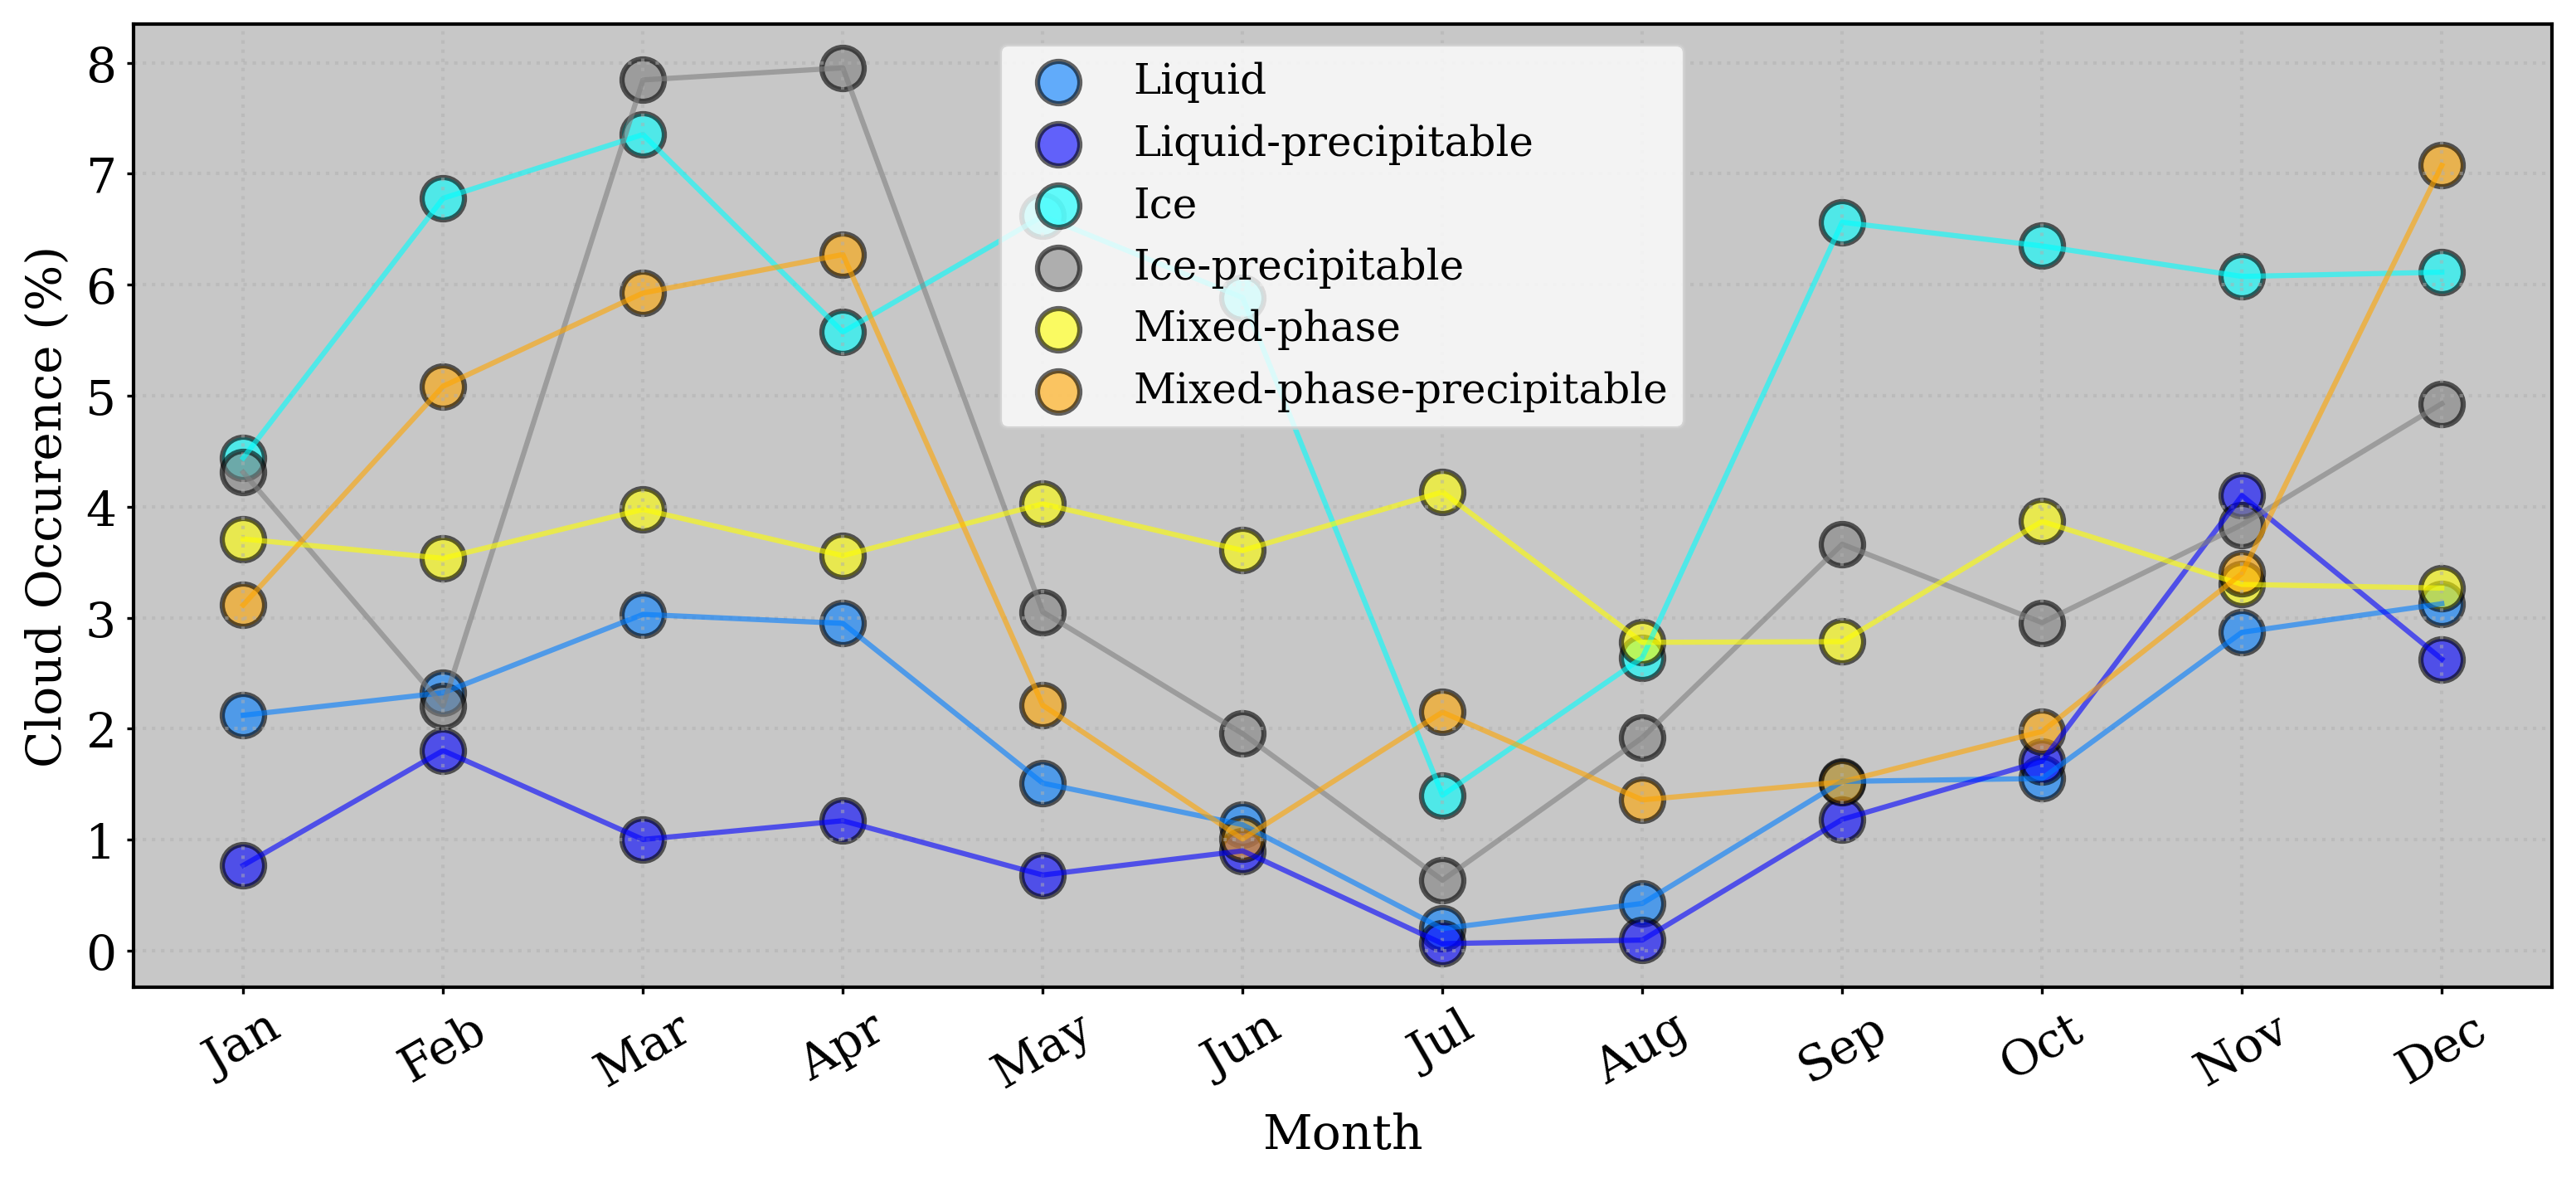
\includegraphics[width=\textwidth]{../../phd_clouds/figures/new_method_monthly_single_layer_frequency}
		\caption{}
	\end{subfigure}
	\caption{On the left, inter-annual frequency of occurrence for single layer clouds (blue), multi-layer clouds (orange), clear sky (green) and noise (red). Right panel, inter-annual single layer cloud occurrence for different cloud categories (see section \ref{sec:new_method}). Each cloud types is indicated in the legend}
	\label{fig:cloud_available}
\end{figure}

Monthly frequency of occurrence is depicted in the right panel of Figure \ref{fig:cloud_available}. Mixed-phase clouds (yellow) exhibit relatively consistent occurrences with slight fluctuations around 3\% and 4\%. Liquid-precipitable (dark blue) has a modest variation with zero occurrence in summer, followed by an increase during the transition to winter, reaching a maximum of 4\% in November, suggesting increased precipitation during fall. Liquid clouds (blue) are more variable, showing a percentage of 3\% in March and December, against zero in summer. Ice clouds (cyan) drop sharply in July and maintain almost constant levels around 5\% and 7\% throughout the rest of the year, indicating hotter temperatures that inhibit ice cloud formation during summer. Ice-precipitable clouds (gray) have a notable peak of 8\% in spring, followed by a decrease in summer (1\%) and an increase in fall, until they reach a local maximum of 5\% during winter. It suggests seasonal variations in ice-related precipitation with maximum in spring, unlike the case of water-related precipitation, which showed a maximum in November. Mixed-phase-precipitable clouds (orange) peak in April (6\%) and December (7\%), indicating higher chances of mixed-phase precipitation towards spring and the end of the year. Overall, ice, precipitating ice, and precipitating mixed-phase clouds have the strongest seasonal pattern, indicating a higher sensibility of ice due to thermodynamic conditions than liquid droplets. Moreover, the precipitation in this region is intrinsically related to ice and mixed phase clouds.

%An important mechanism associated with temperature decreases and responsible for extreme rainfall in Eastern Spain is the occurrence of cut-off lows (COLs). COLs account for nearly all rain events in Valencia, Spain \citep{ferreiraCutOffLowsExtreme2021}, and are likely to affect the Granada station as well. This influence is attributed to the easterly wind component of COLs formed in the warm Mediterranean \citep{porcuStudyCutoffLow2007}, which can reach the station, bringing humidity and cold air masses that favor cloud formation. In Valencia, \cite{ferreiraCutOffLowsExtreme2021} reported the rainiest days occurring in winter, with extreme rainfall events in spring and fall, aligning with our observations. 

During the summer temperatures are higher and just a few non-precipitating clouds were observed at our station. These clouds can be related to convection since we will observe that they have larger thickness and ice water content (IWC) at higher altitudes. Besides elevated temperatures, the Iberian Peninsula experiences a large low-pressure area over northern Africa, with high-pressure systems over the Atlantic Ocean and eastern and central Europe. This results in easterly winds over Andalusia, transporting moisture from the Mediterranean Sea in summer \citep{f.j.bello-millanSimulationsTornadicSupercell2024}. This combination of high temperatures and humidity can create an environment conducive to storm formation in Granada during the summer. In this context, the few clouds observed in summer are likely related to convectively formed cumulus or cumulonimbus clouds. This will be more evident when studying their physical properties in further sections.

Next, the daily cycle of cloud occurrence should uncover the influence of temperature around mid-day, when the solar radiance is more intense. Although we already discuss the influence of synoptic and local phenomena in cloud formation, convection clouds should appear in the diurnal cycle. Figure \ref{fig:cloud_occurence_daily_cycle} displays the diurnal cycle per season, showing no convection for any type of cloud during summer, fall and winter. Despite that fall shows an increase of ice clouds around mid-day, they are probably cirrus clouds, since their median base height and thickness are 8.5\,km and 1.5\,km, respectively (see Figure \ref{fig:cloud_macrophys}).

\begin{figure}[H]
	\centering
	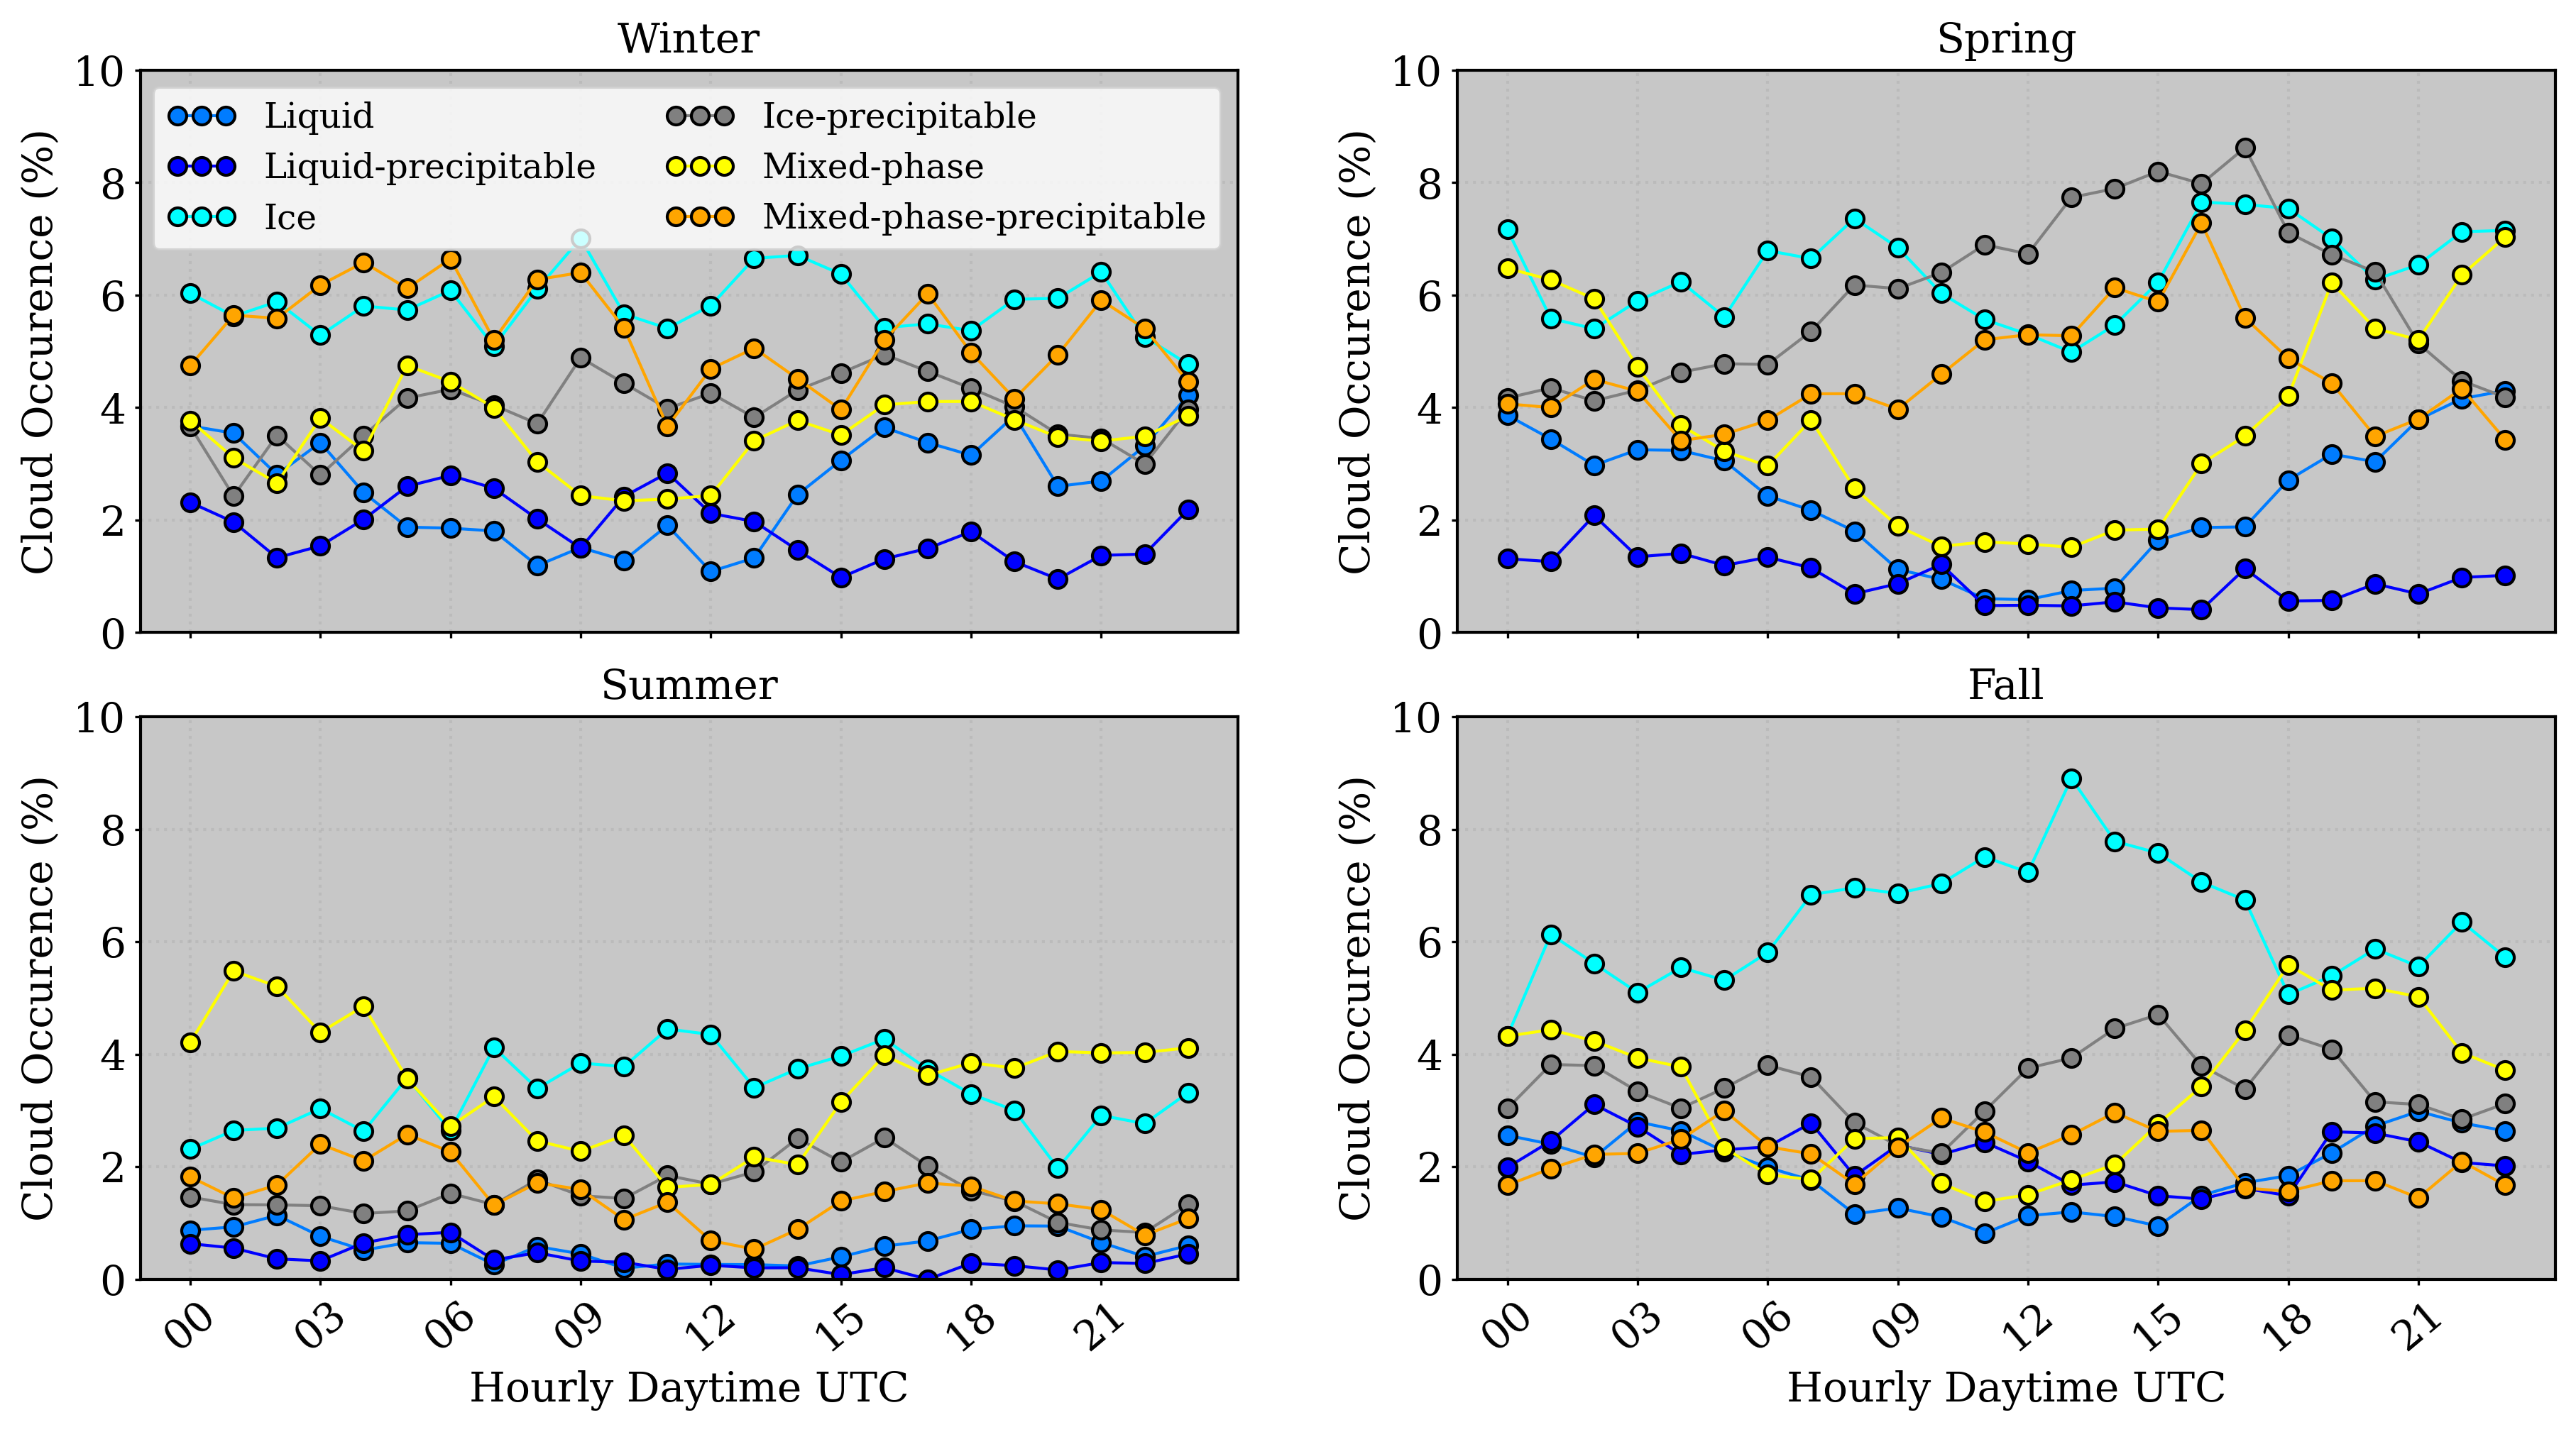
\includegraphics[width=.9\textwidth]{../../phd_clouds/figures/hourly_seasonly_single_layer_frequency}
	\caption{Daily cycle of cloud occurrence per season. The season is indicated in the title of each figure, where winter and spring are in the first row, and summer and fall in the second row. The color of each cloud category is indicated in the legend}
	\label{fig:cloud_occurence_daily_cycle}
\end{figure}

However, spring shows a possible presence of convective clouds, with a slight peak of occurrence for Ice-precipitable and Mixed-phase-precipitable clouds between 09:00 and 21:00 UTC. Different from non-precipitating clouds which reached a minimum around mid-day, these clouds doubled the occurrence from 4\% at 00:00 to 8\% at 16:00-17:00 UTC. These observations are consistent with the findings of \cite{shahiAssessmentSpatiotemporalVariability2022}, where convection-permitting models of the Iberian Peninsula (IP) captured high values of mean precipitation during spring. Additionally, \cite{alexandrerios-entenzaMoistureRecyclingIberian2014} revealed that specific synoptic conditions, such as a reduction in the strength of the zonal circulation, can favor local and mesoscale convection during spring in the western region of the IP. This analysis confirms that the maximum cloud and rain occurrence observed during peak sunlight hours may be strongly associated with local convection. 

\subsection{Seasonal patterns in cloud base, top, and thickness}

Seasonal evolution of cloud base height, top height and thickness are displayed in Figure \ref{fig:cloud_macrophys}. Each color represents a cloud type, where liquid clouds are in blue, ice clouds are in gray and mixed-phase clouds are in orange. Also, the lightest colors represent non precipitating clouds, and the darkest colors represent precipitation clouds. Thus, through cloud base analysis, precipitating clouds exhibit a significantly lower cloud base height (top panel) compared to non-precipitating clouds, as well as a narrower distribution. Regarding non-precipitating ice clouds, they possess the highest cloud base heights, with median values around 8\,km. The ice clouds with base height above the 50/75th percentile can be normally associated with cirrus clouds. Next, non-precipitating mixed-phase clouds have the second highest cloud base, showing considerable variability, except during summer, when values stabilize at 5.5 km. Also, these clouds present a higher base in fall, where the 50th percentile reaches 6.5 km. Differently, the precipitating mixed phase clouds have much less variability and higher cloud base at 4.5 km in summer, as expected. For non precipitating liquid clouds, cloud bases are highly variable during summer, achieving significantly different heights compared with other seasons. Overall, in summer, precipitating mixed-phase clouds, and ice precipitating clouds demonstrate elevated cloud base heights, attributed to the relatively high temperatures and low humidity at this season. Liquid clouds also have elevated base height in summer, however only a few cases were registered, with 50th and 75th percentiles around 4 km and 6 km, respectively. These clouds can be related to stratocumulus and stratus clouds, which were dis-coupled from cumulonimbus at the final stage in summer. 

Following, precipitating clouds also have significantly lower median cloud top height (panels at the center of Figure \ref{fig:cloud_macrophys}) compared to non-precipitating clouds and exhibit a narrower cloud top distribution, except in the case of ice clouds. Non-precipitating ice clouds have median cloud tops around 9-10 km, while ice-precipitable clouds demonstrate highly variable cloud tops. Given their well-defined cloud bases, these clouds exhibit greater cloud thickness, indicative of storm activity at our station.
The cloud tops for liquid clouds mirror the variability of their cloud bases, especially during summer. These clouds exhibit a well-defined cloud thickness, with non precipitating liquid clouds having a thickness around 300 m and precipitating liquid clouds reaching up to 500 m.
Non precipitating mixed-phase cloud tops also present high variability. Nevertheless, they displayed a well-defined cloud thickness, with similar distribution along seasons. Their median cloud thickness is around 400 m, increasing to 500 m for the precipitating case (dark orange), with slightly higher values in summer. In general, non-precipitating mixed-phase clouds have median cloud tops around 7 km during spring, summer, and winter, but reach 8.5 km in fall. Then, precipitating mixed-phase clouds have cloud tops around 3 km in spring, fall, and winter, peaking at 7 km in summer.

\begin{figure}[H]
	\centering
	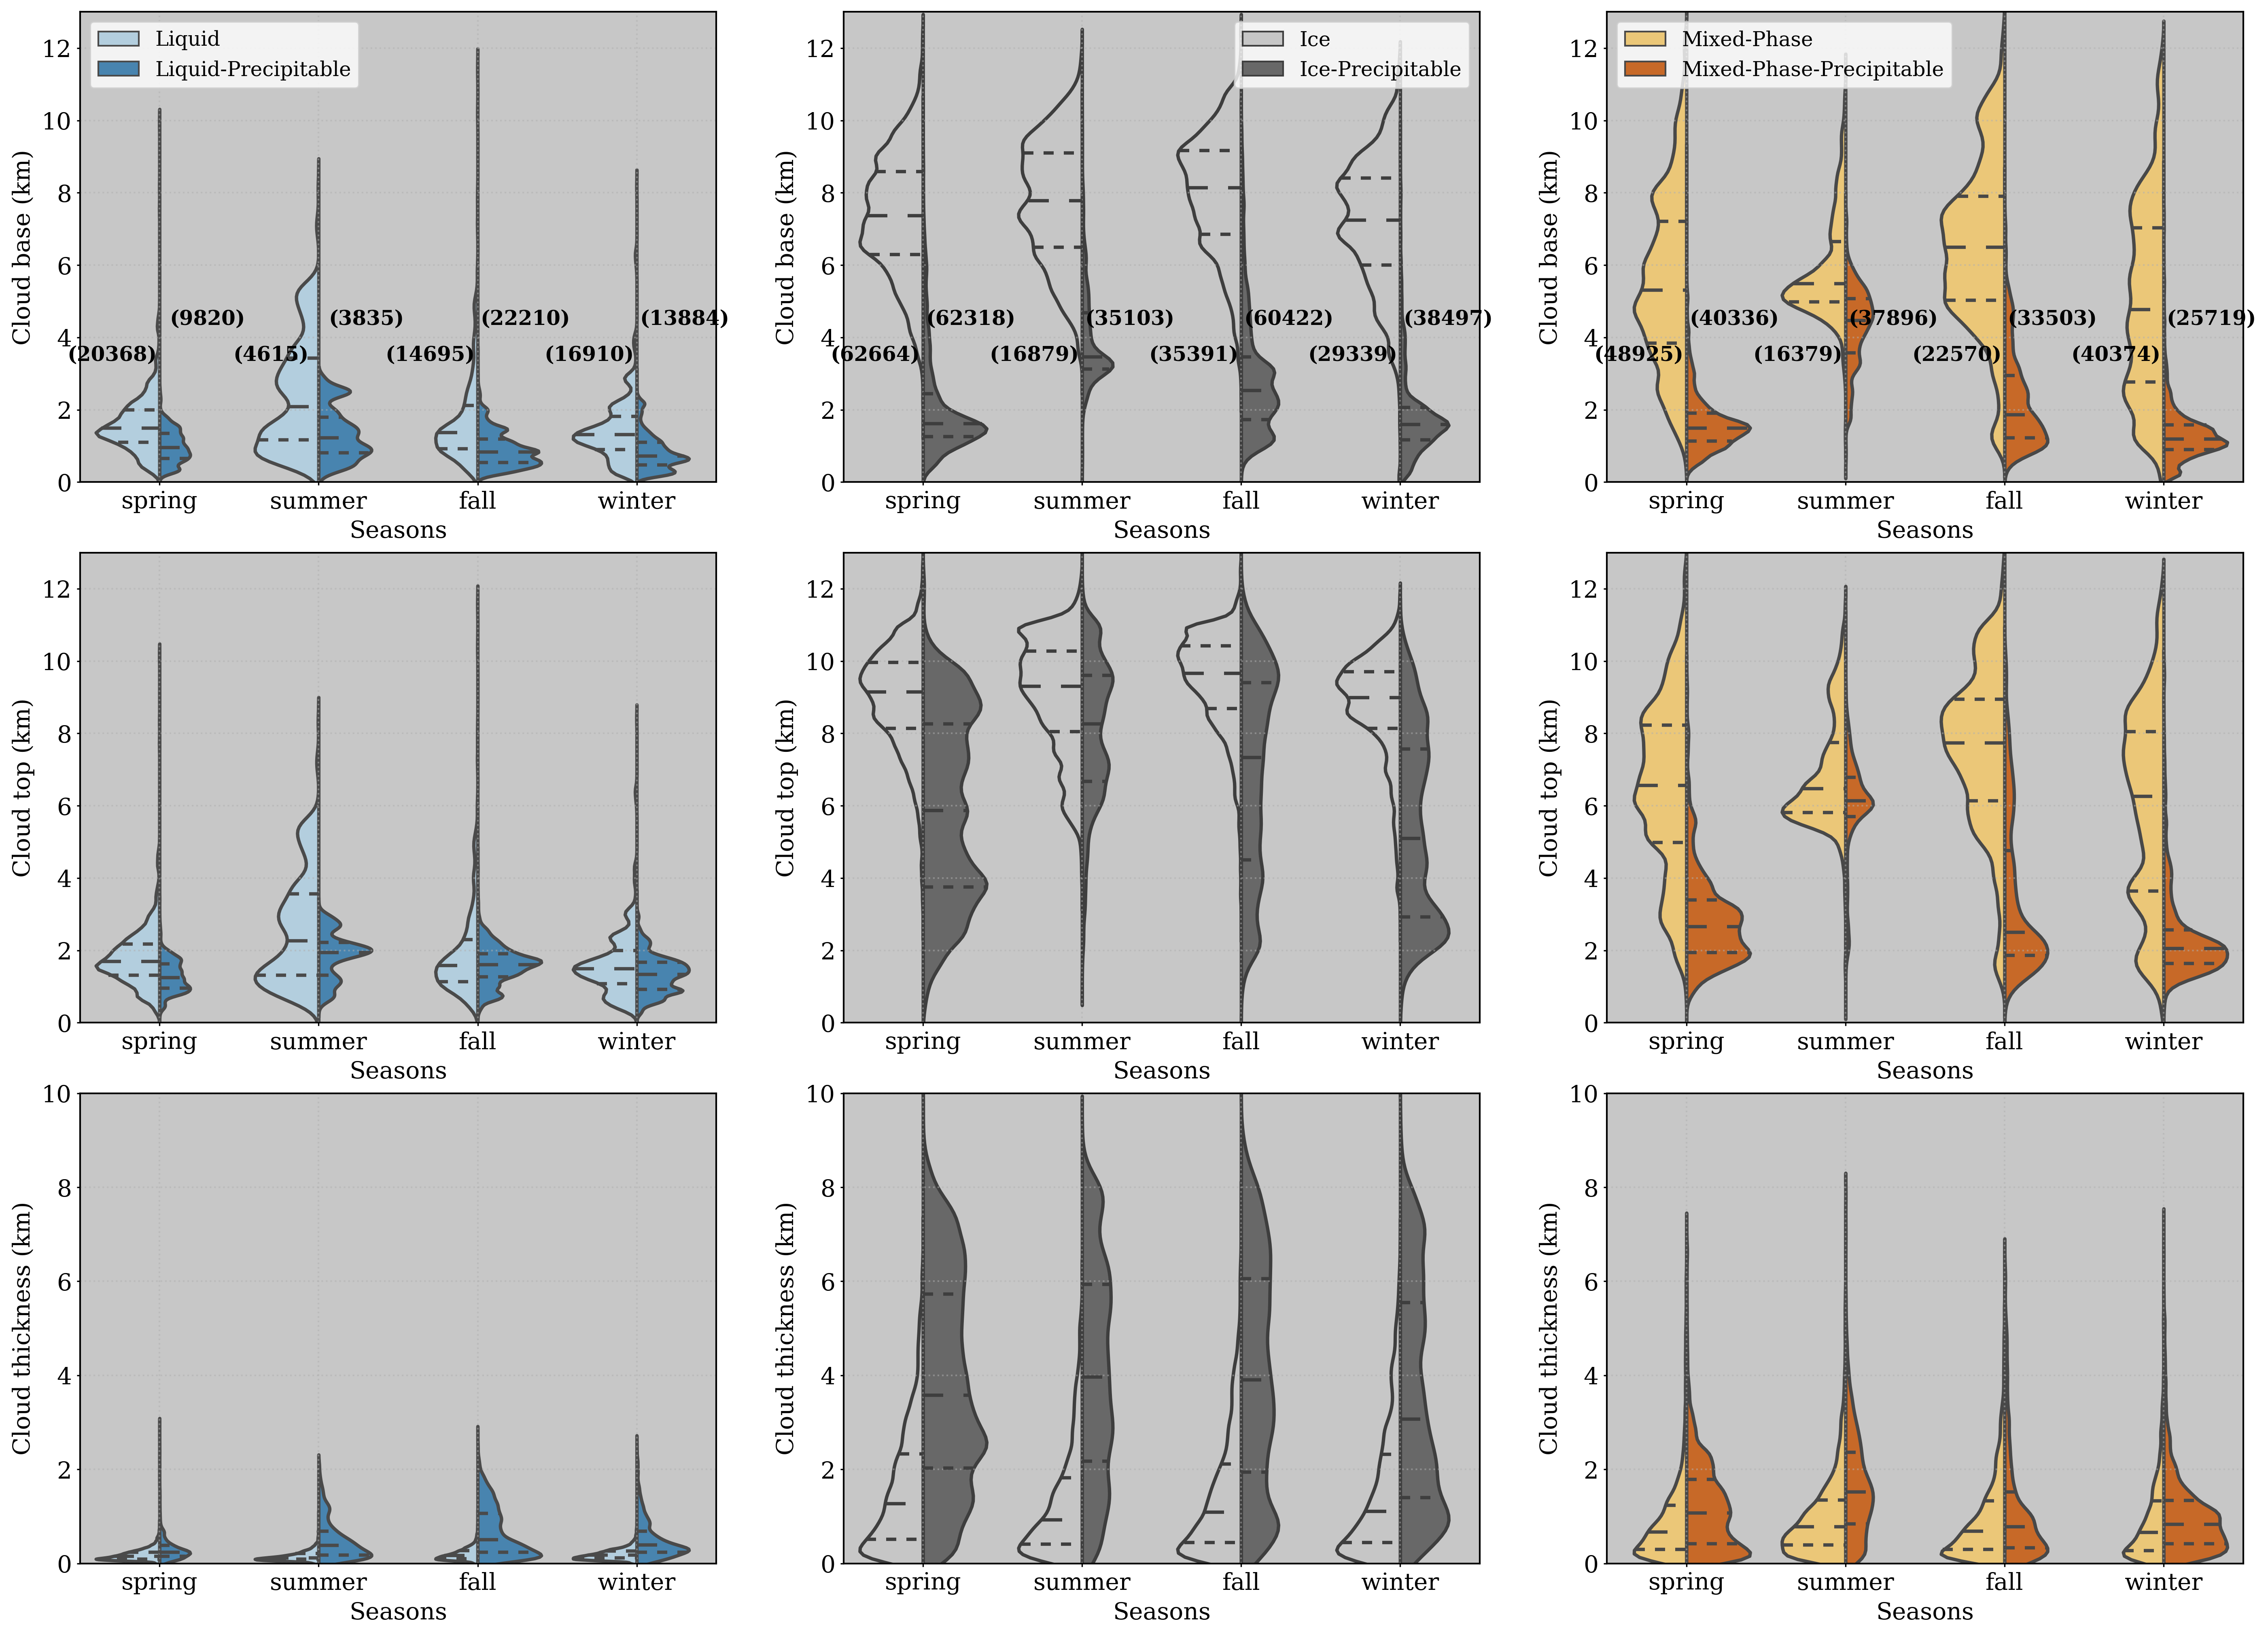
\includegraphics[width=1.\textwidth]{../../phd_clouds/figures/new_method_cloud_prop_violin_season}
	\caption{Seasonal evaluation of cloud base height, top height and thickness. The cloud bases are in the first row, cloud tops in the second row and cloud thickness in the third row. Also, each cloud type is indicated in the legend, where liquid clouds are in the first column, ice clouds in the second column and mixed-phase clouds in the third column. Finally, the dashed lines are indicating the 25/50/75th percentiles}
	\label{fig:cloud_macrophys}
\end{figure}

Overall, ice-precipitable clouds exhibit the greatest cloud thickness, followed by ice, mixed-phase-precipitable, mixed-phase, liquid-precipitable, and liquid clouds. It is important to note that, despite Cloudnet post-processed data being corrected for liquid attenuation, cloud tops for precipitating clouds with higher thickness can be underestimated due to high liquid attenuation.

\subsection{Cloud microphysics properties}\label{sec:cloud_microphys}

\subsubsection{Liquid clouds}

The monthly median profiles of LWC shows high variability of LWC in function of height for liquid clouds (Figure \ref{fig:LWC_liq}, right panel, marked by hot colors and constant lines of 1000 mg m$^{-3}$). For particular months such as February, March and April, a notably variability below 1 km and within 2.5 and 4 km (right panel of Figure \ref{fig:LWC_liq}) is observed. Nevertheless, above 500 m, really high values observed in the monthly profiles are not representative of the entire season as can be seen in the left panel of Figure \ref{fig:LWC_liq}. This figure shows no clear pattern with altitude at any season, LWC is generally presenting a random fluctuation around to 50 mg m$^{-3}$. Differently, below 500\,m, a sharp peak of about 500 mg m$^{-3}$ can be clearly identified in spring. This peak is related to liquid clouds during the springs of 2020, 2021 and 2022 (not shown), at this period. Except for the near surface largest LWC observed in spring, no clear differences were observed between seasonal profiles. Following, summer exhibited a lack of liquid phase clouds, with some elevated LWC at higher levels as shown in the left panel of Figure \ref{fig:LWC_liq}.

Next, the average liquid water path (LWP) (bottom panel of Figure \ref{fig:LWC_liq}, black star) shows a considerable variability of LWP from January to June (also early fall). It highlights a very wide variety of liquid clouds in these months. Also, a notable increase in the median LWP occurs in April, aligning with their maximum cloud occurrence. From August to October, there is a gradual increase in average LWP (marked by the black star), while the median stays stable. This trend corresponds with the increased occurrence of liquid clouds from summer to fall, impacted by different mechanisms of cloud formation. Since these months reported just a few occurrences of liquid clouds, as can be checked by the blue line, which shows the number of cloud profiles per month, their statistics will be much more sensible to these mechanisms. As a result LWP in summer is the smallest, and there is no significant difference between the average and the median.

\begin{figure}[H]
	\centering
	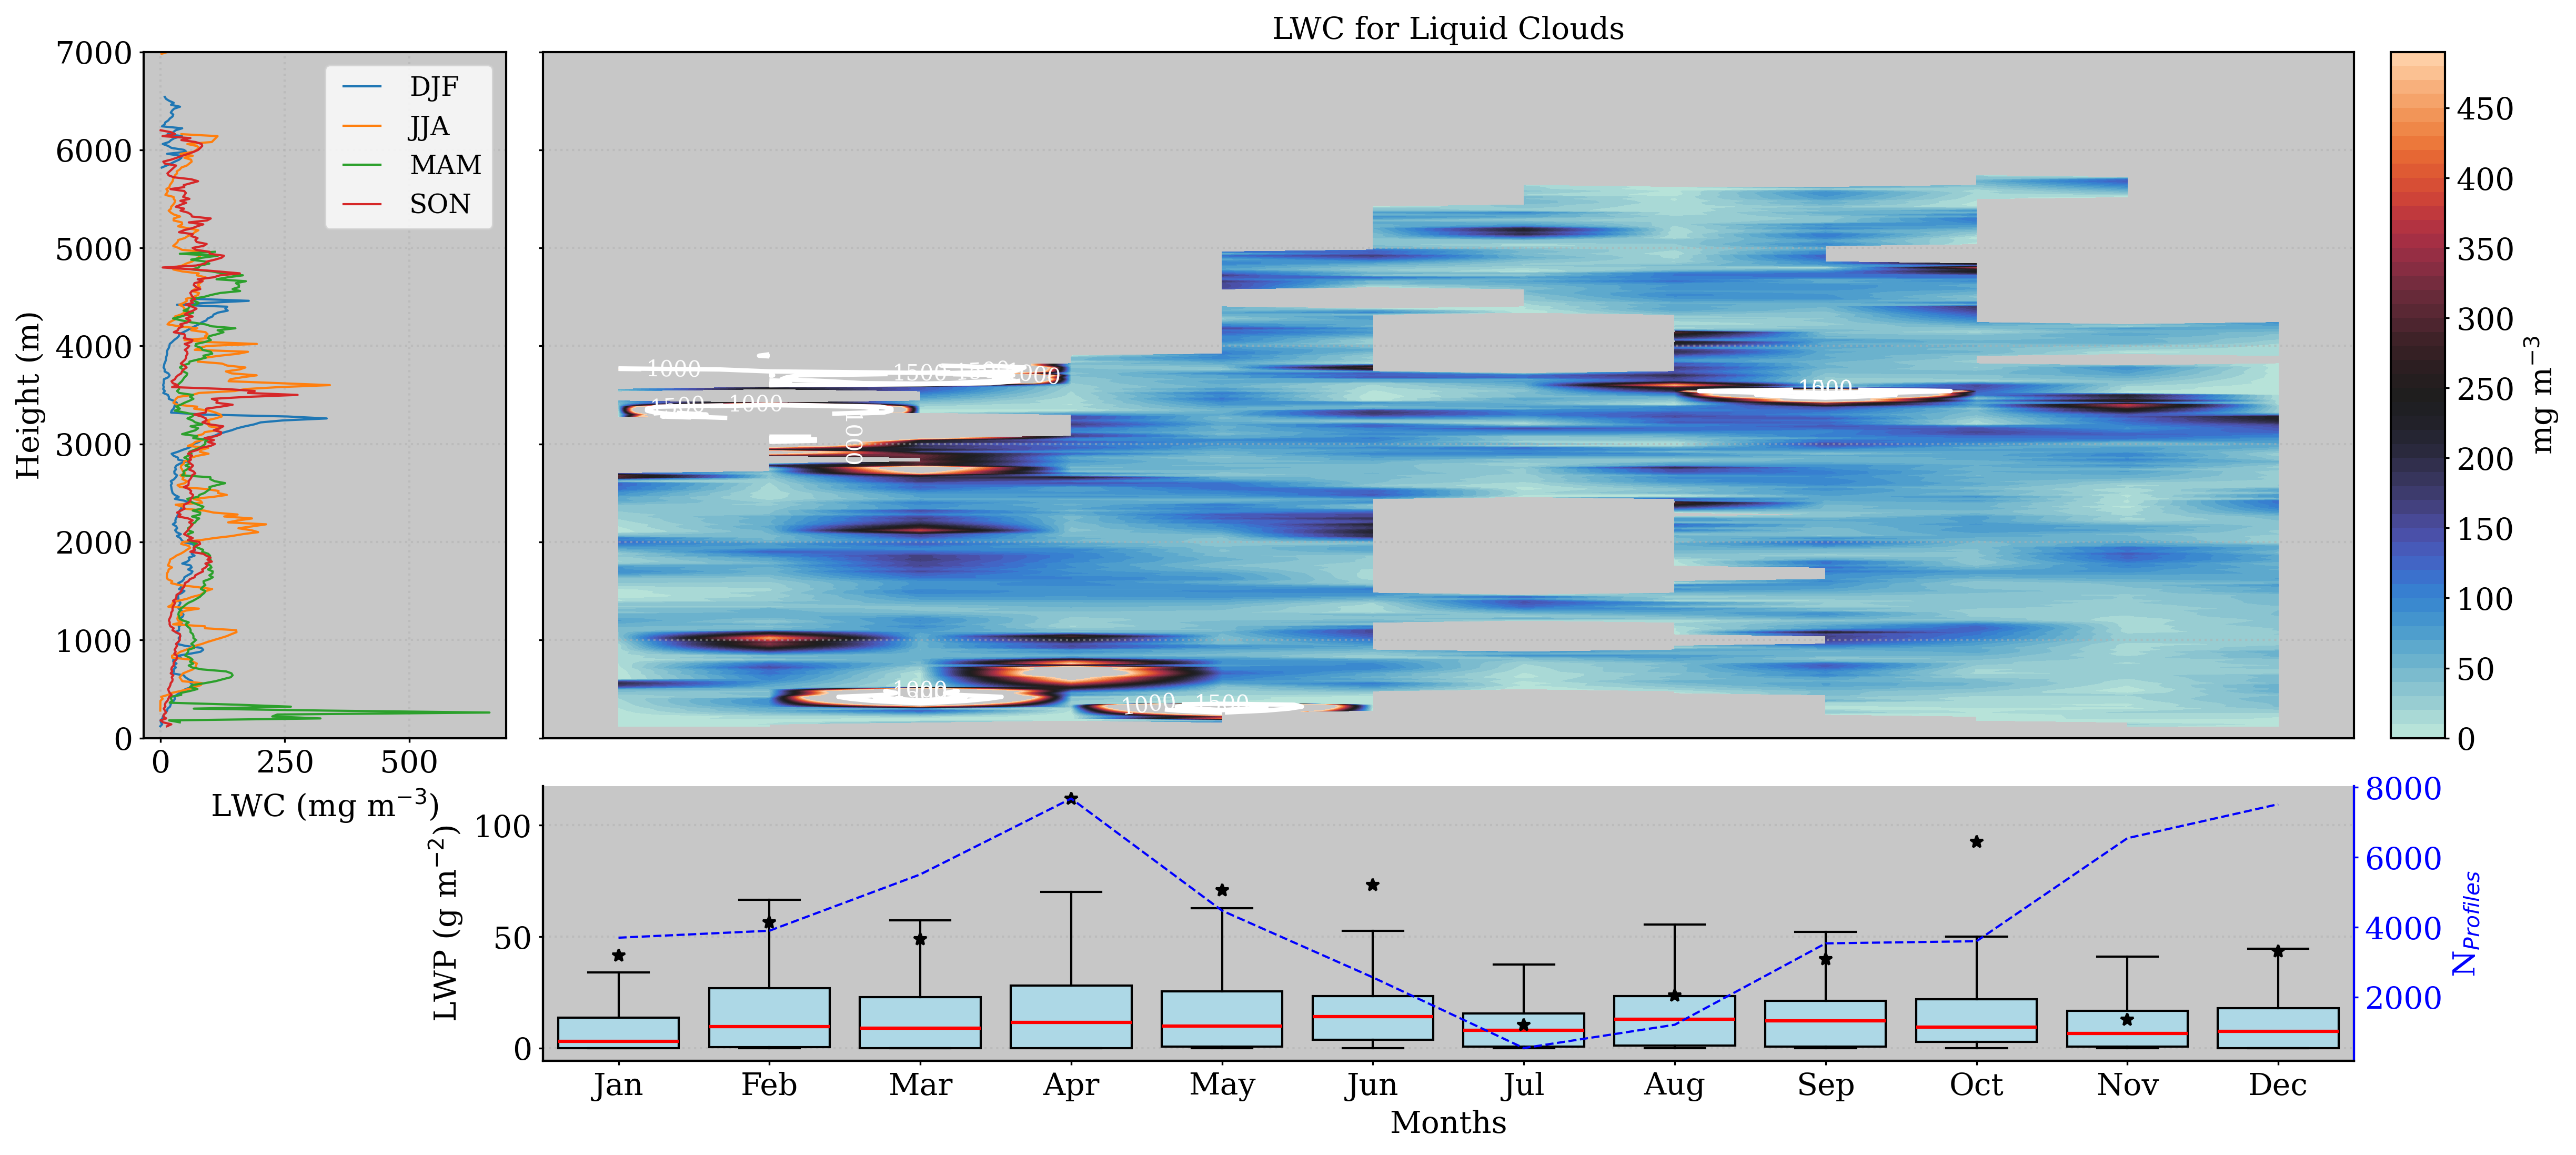
\includegraphics[width=.9\textwidth]{../../phd_clouds/figures/grouped_by_month_evolution_for_lwc_Liquid_mesh}
	\caption{Seasonal and monthly average of liquid water content (LWC) and liquid water path (LWP) for liquid clouds. Left panel shows the seasonal median profiles of LWC. 
		%      where the shaded area indicates the standard deviation divided by 10. 
		Right panel shows the monthly median profiles of LWC and monthly box-plot of LWP in the bottom. For the boxplots, medians are denoted by red lines and the average by black stars.} 
	\label{fig:LWC_liq}
\end{figure}

In terms of droplet effective radius, liquid clouds are well consistent throughout the year, showing small differences in terms of median values (top panel of Figure \ref{fig:DER_liq}), mostly ranging between 5 and 9 $\mu$m. There is no discernible pattern in $r_{liq}$ across seasons, with higher altitudes weakly correlating to larger droplet sizes. In addition, there are almost no liquid droplets above 4 km, just a few occurrences in summer and early fall were registered.

However, the $r_{liq}$ is generally stable around 5 $\mu$m, with a small decrease in July, when almost no clouds were registered. The seasonal profiles confirm the uniformity in $r_{liq}$ distribution with height, showing minimal variation with altitude. It suggests a consistent cloud composition and droplet size throughout different atmospheric conditions. These findings underscore the stable nature of liquid clouds in terms of droplet size and LWC. Normally, these clouds have a small thickness, do not presenting a wide range of $r_{liq}$

\begin{figure}[H]
	\centering
	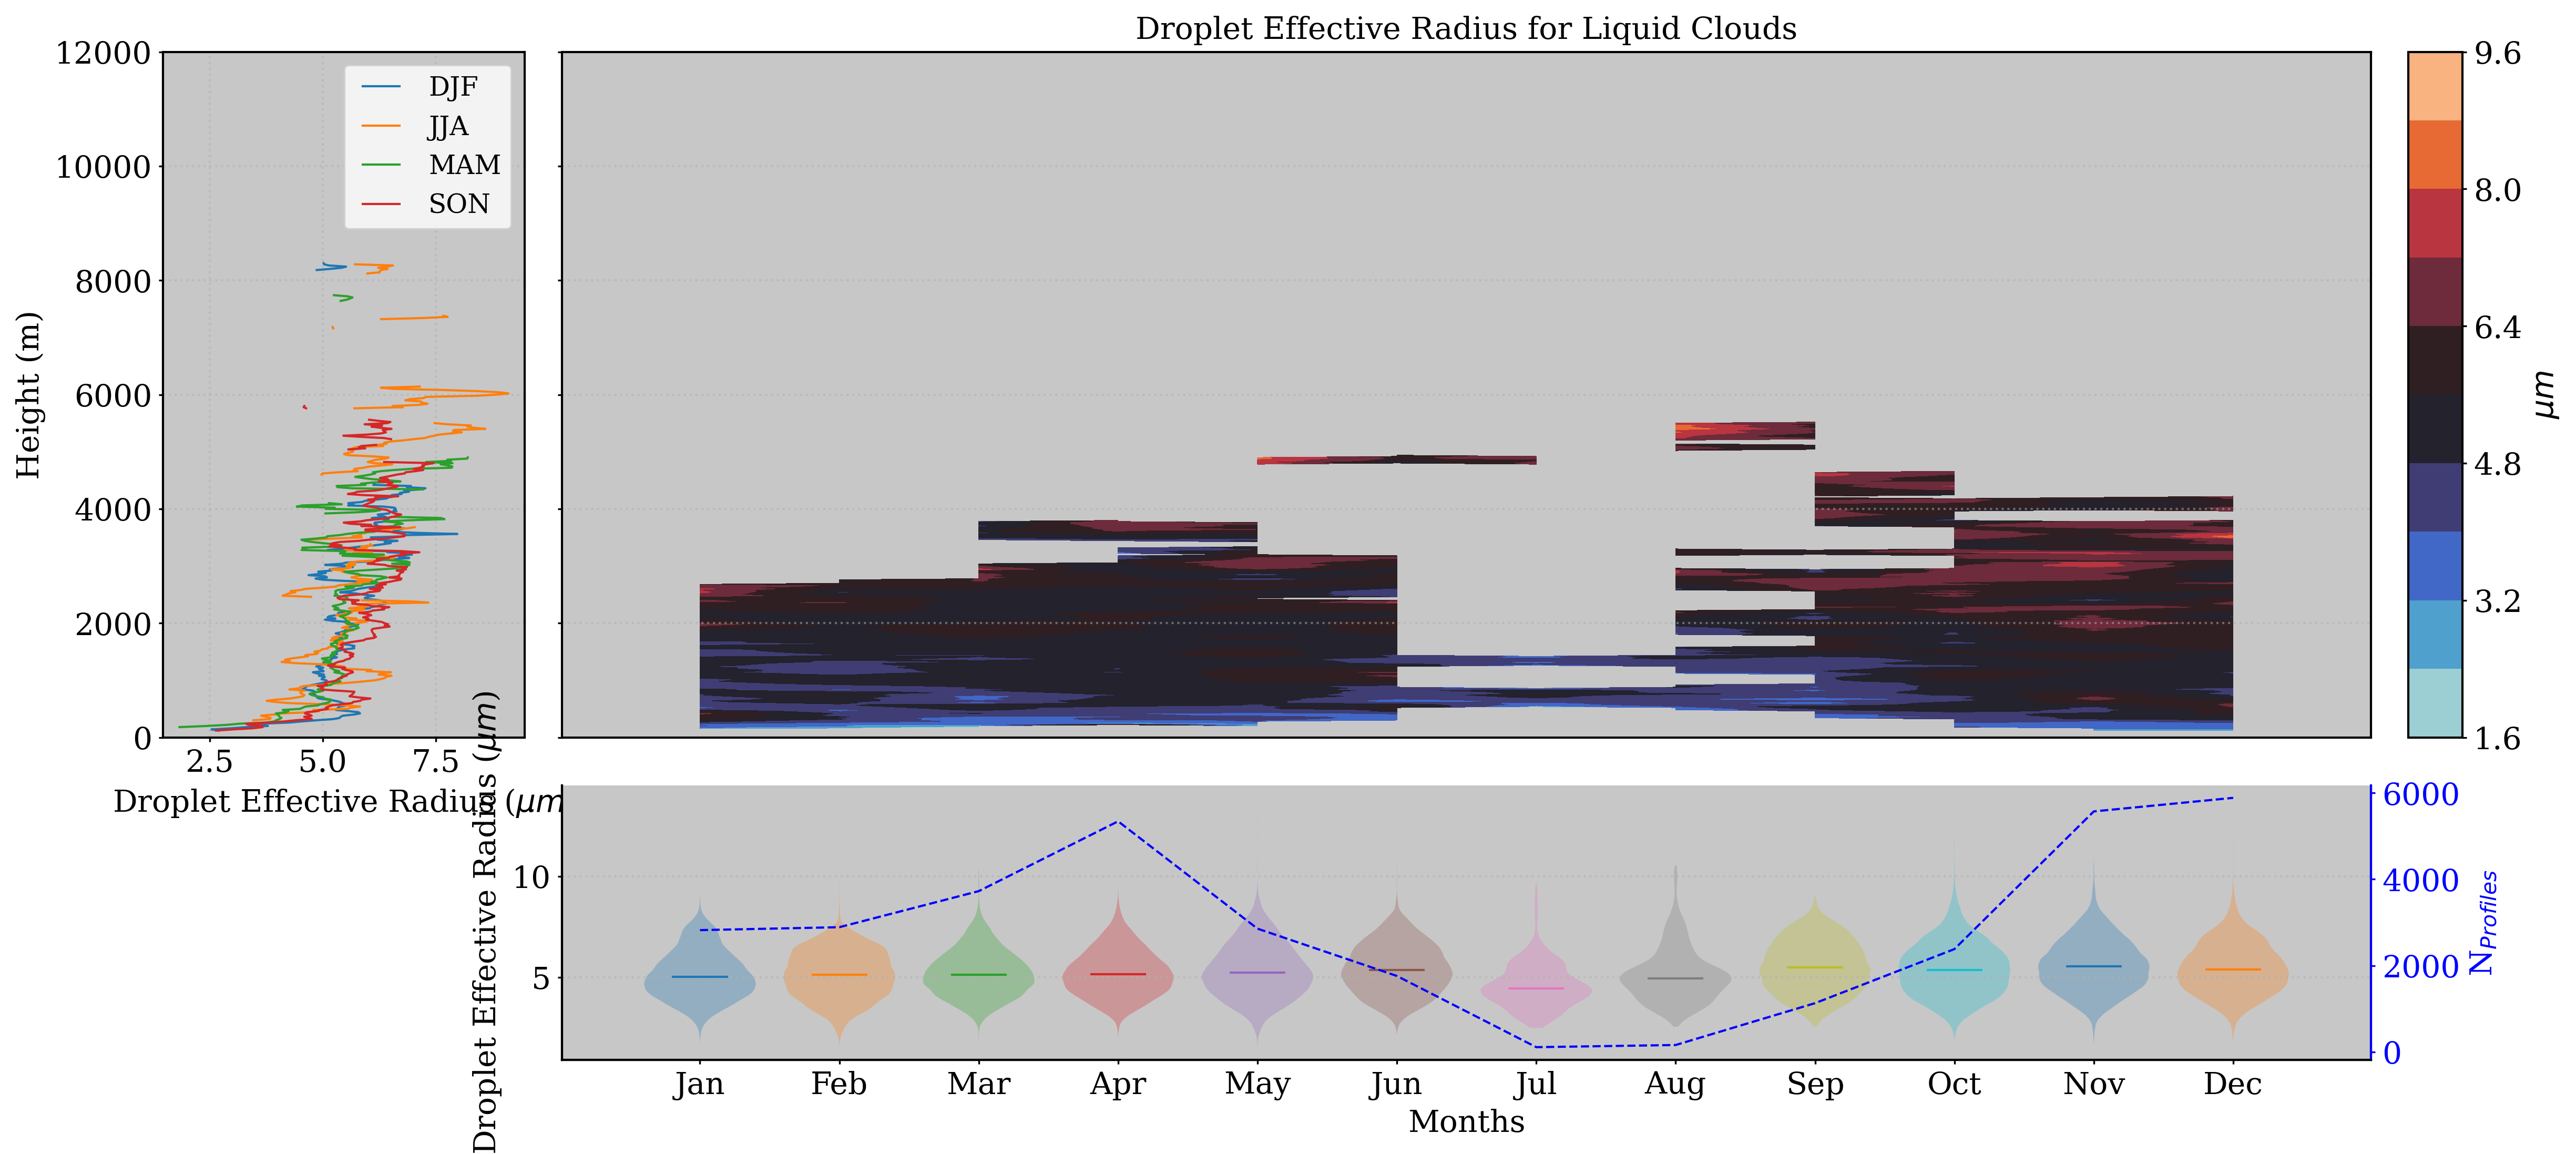
\includegraphics[width=.9\textwidth]{../../phd_clouds/figures/grouped_by_month_evolution_for_der_Liquid}
	\caption{Seasonal and monthly statistics on droplet effective radius ($r_{liq}$) distribution for liquid clouds. Left panel shows the seasonal median profiles of droplet effective radius. Top-right panel shows the monthly profiles of the median $r_{liq}$, while the bottom-panel displays the size distribution of $r_{liq}$ by months.}
	\label{fig:DER_liq}
\end{figure}

For precipitating liquid clouds, significant liquid water content (LWC) is primarily found below 3 km (top-right panel of Figure \ref{fig:LWC_pre_liq}), consistent with their median top heights. Next, regions with significant values of liquid water content show broader areas, which is expected as these clouds are thicker than purely liquid clouds. Monthly median profiles indicate that higher amounts of liquid water content occurs in later fall, winter and spring. However, the highest amount of LWC is identified in June (early summer), very close to the ground (300 m), which is related to only a few cases of these clouds registered in summer (see the blue line in the bottom panel). Then, in the rest of summer and early fall, atmospheric water content is almost zero. In spring, significant values are found even closer to the surface, explained by relatively humidity months in 2020, 2021, and 2022 as already observed for non precipitating liquid clouds. At the last, winter shows a peak of LWC of about 
250 mg m$^{-2}$ at 2 km. 

Overall, the seasonal profiles of LWC emphasizes a clear increase of LWC in function of height during fall, winter and summer. For the last, two peaks of 250 mg m$^{-3}$ are clearly identified at 2 and 3 km, respectively. This season presented more variability with height, showing more peaks of LWC in function of height. Next, fall and winter also presented a peak of about 250 mg m$^{-3}$ at 2 and  2.5 km, respectively. In terms of LWP, Figure \ref{fig:LWC_pre_liq} below indicates substantial variability of LWP in January, suggesting a diverse variety of liquid clouds during this month. In contrast, spring exhibits relatively consistent LWP across its months, reflecting a stable period for precipitating liquid clouds. In these months, their median stays below 50 g m$^{-2}$, and summer has even less LWP, except for June, as previously observed.

\begin{figure}[H]
	\centering
	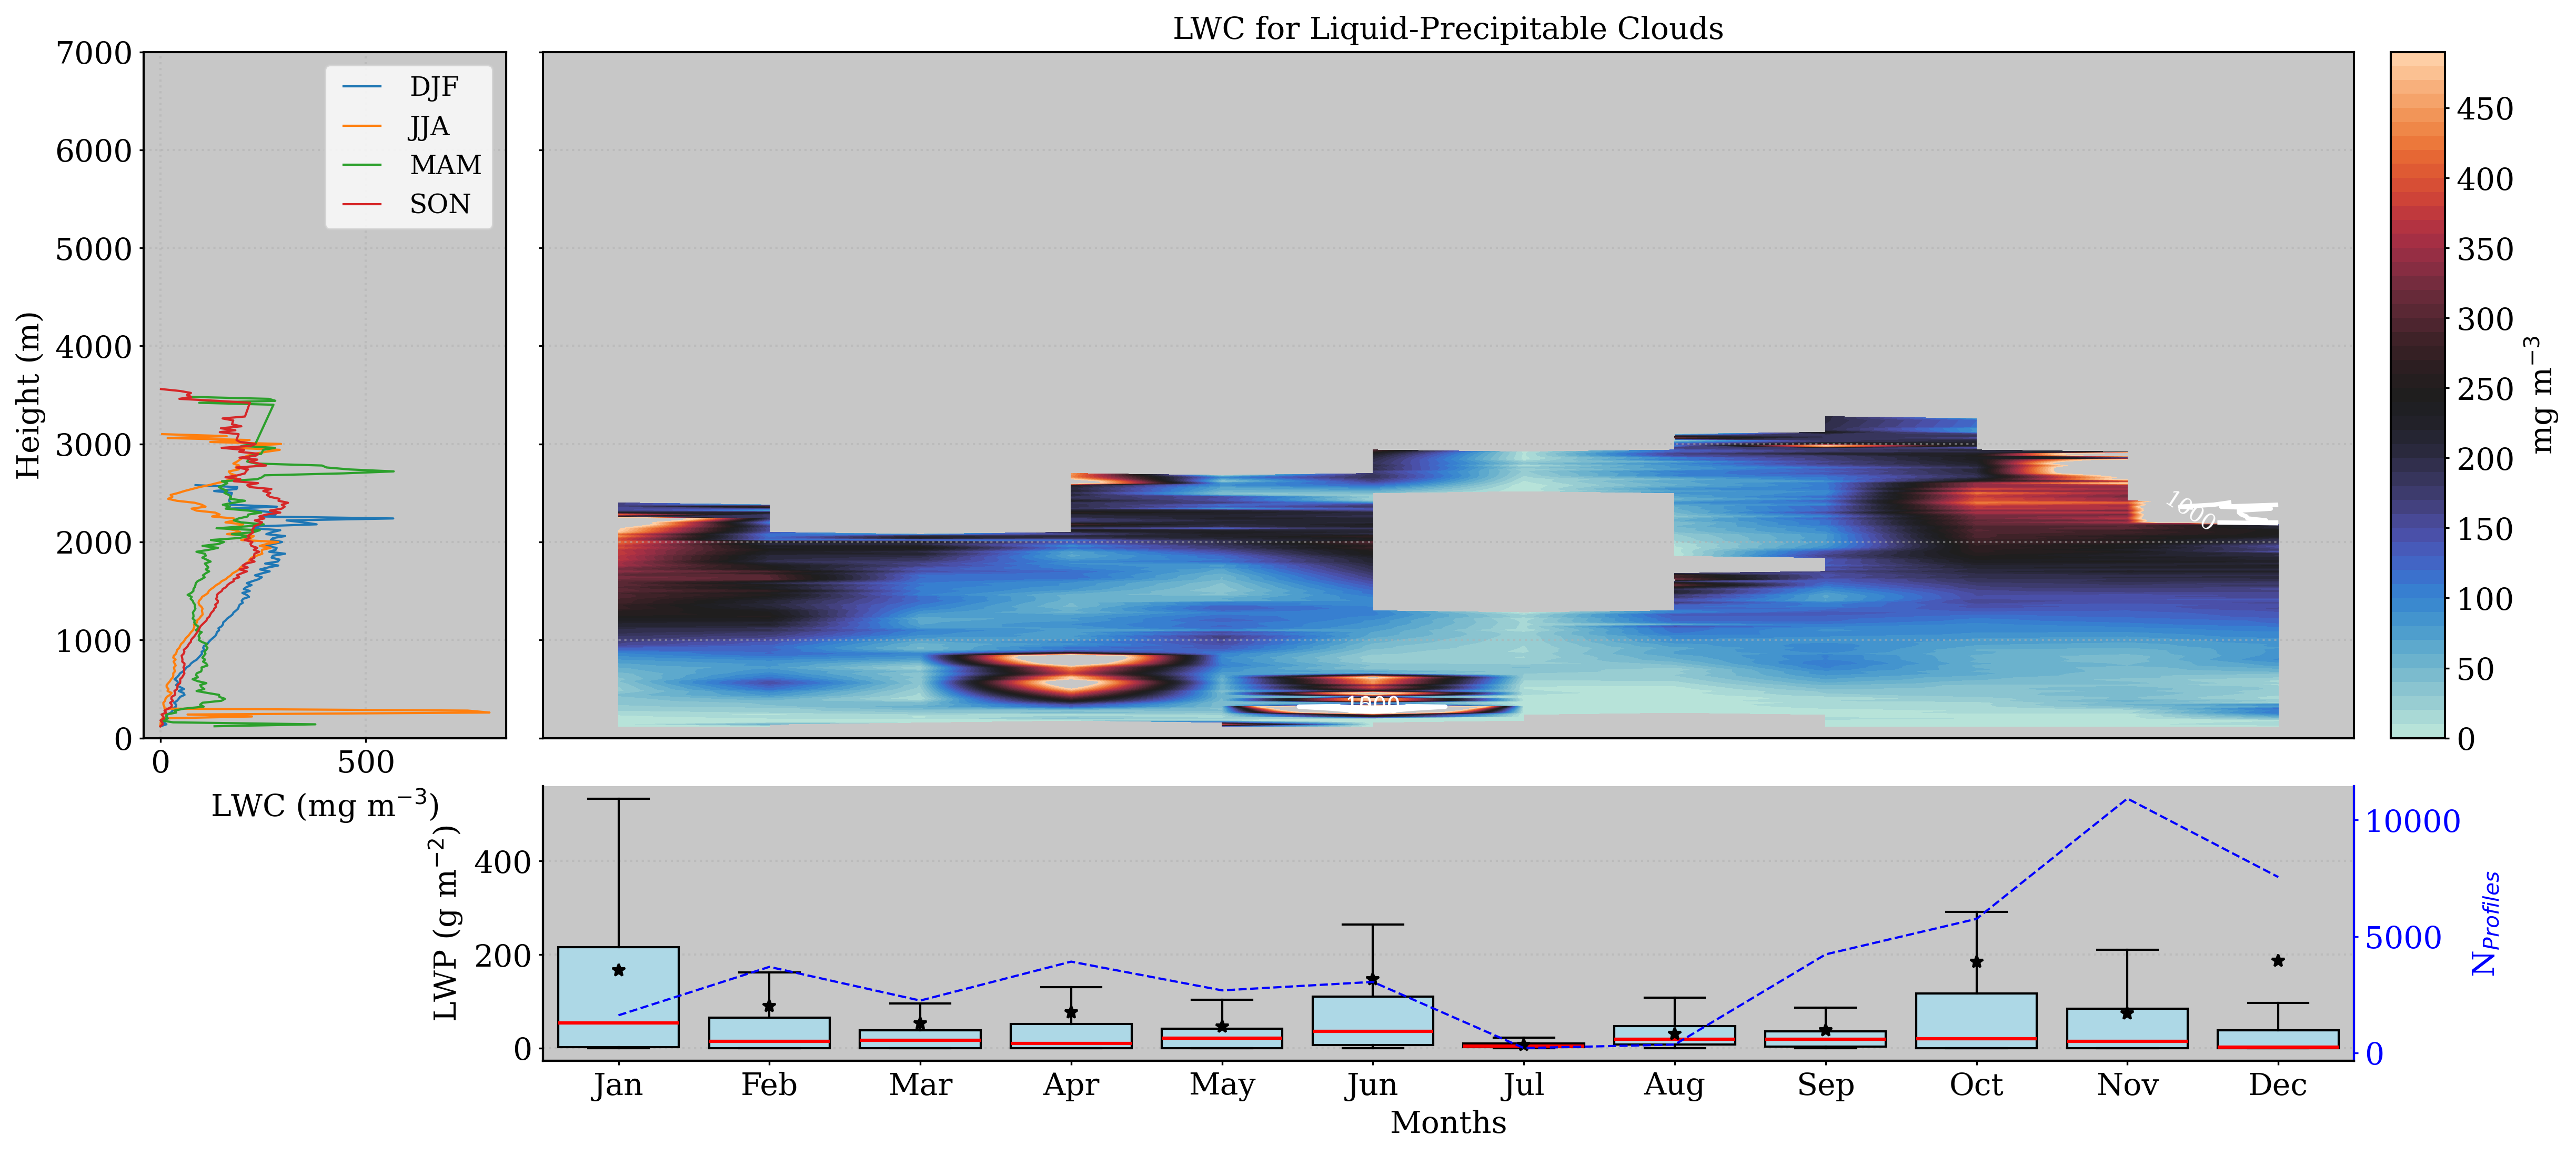
\includegraphics[width=.9\textwidth]{../../phd_clouds/figures/grouped_by_month_evolution_for_lwc_Liquid-Precipitable_mesh}
	\caption{Same as Figure \ref{fig:LWC_liq}, but for precipitating liquid clouds.}
	\label{fig:LWC_pre_liq}
\end{figure}


Different for the purely liquid clouds, precipitating liquid clouds demonstrated radically different seasonal profiles of median $ r_{liq} $ (see Figure \ref{fig:DER_pre_liq}). In spring and summer, the $ r_{liq} $ is smaller than fall and winter the closer to the ground, as can be seen by light blue and warm colors. In addition, $ r_{liq} $ in fall are the largest, often around 15 $\mu$m below 2 km. These sizes are normally related to drizzle droplets, which are more present in this season. The highest median $ r_{liq} $ on the ground in the left panel of Figure \ref{fig:DER_pre_liq} is also related to drizzle particles. This panel also shows that summer and winter exhibit similar $ r_{liq} $ values up to 2 km of altitude, around 10 $\mu$m, decreasing to approximately 5 $\mu$m at 4 km. On the other hand, spring shows an increase of $ r_{liq} $ from 5 $\mu$m to a peak of 15 $\mu$m around 3 km altitude. 

Their monthly size distribution in the bottom panel displays different size distributions over the year, where higher median values are found in fall as already observed, specially in November. During spring and early summer, the median is maintained around 10 $\mu$m, then decreases in summer, and increases again in fall as expected.

\begin{figure}[H]
	\centering
	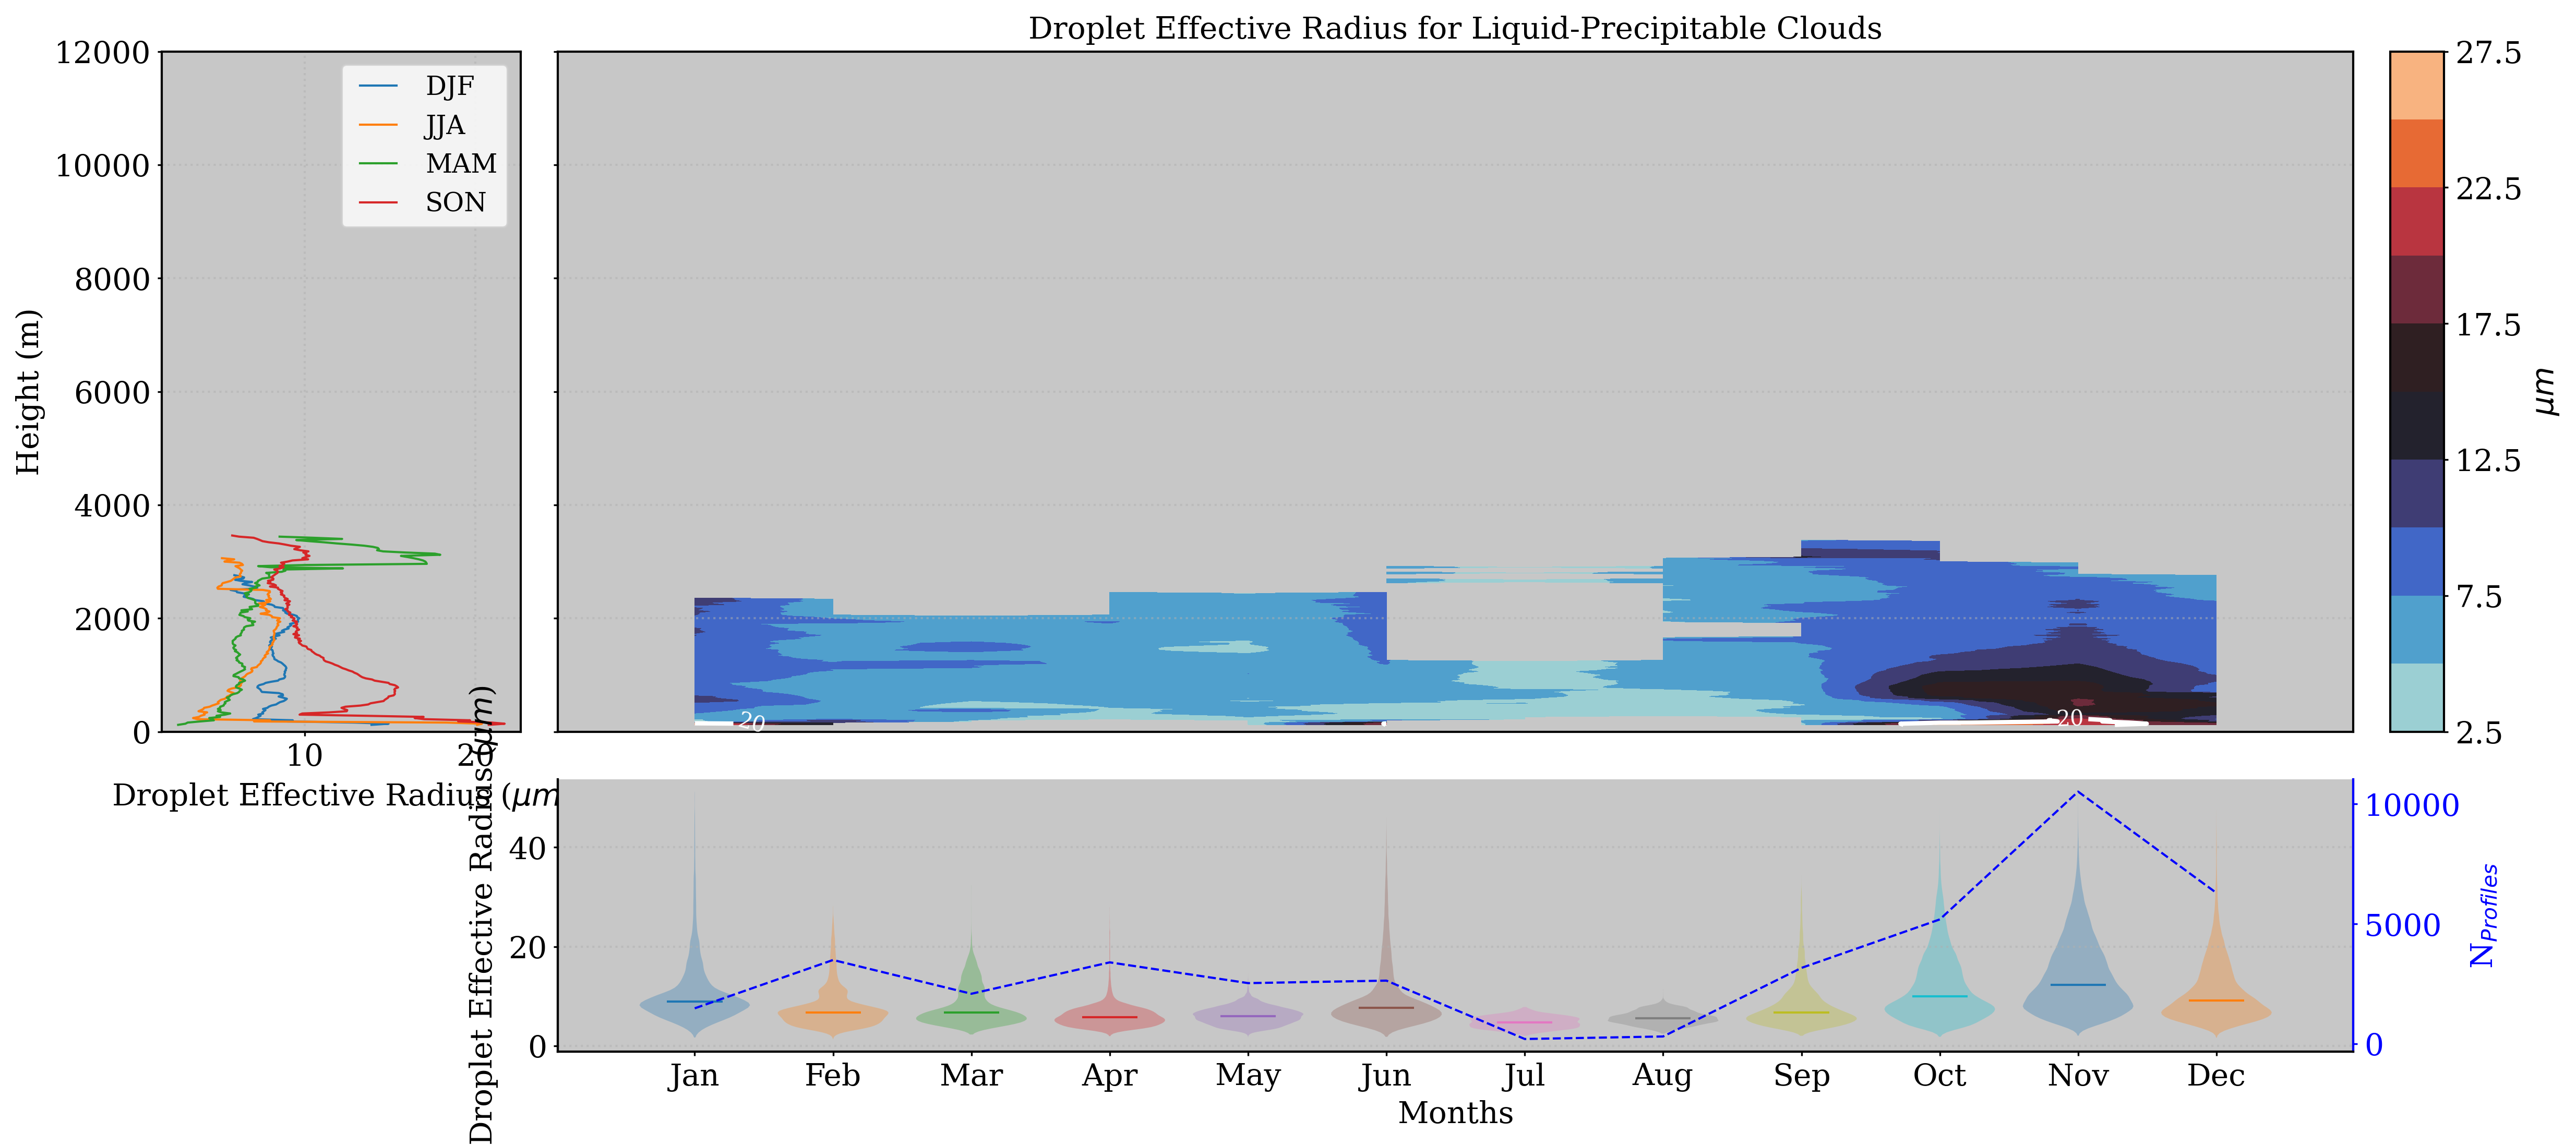
\includegraphics[width=.9\textwidth]{../../phd_clouds/figures/grouped_by_month_evolution_for_der_Liquid-Precipitable_mesh}
	\caption{Same as figure \ref{fig:DER_liq}, but for precipitating liquid clouds.}
	\label{fig:DER_pre_liq}
\end{figure}

Liquid clouds are challenging to analyze due to their low frequency of occurrence. They exhibit significant variability with height, making it difficult to discern seasonal differences in liquid water content (LWC) profiles, except at low levels. Near the surface, LWC is much higher in spring, though their droplet size ($r_{liq}$) remains relatively constant around 5 $\mu$m. In contrast, precipitating liquid clouds display a more pronounced seasonal pattern, with higher LWC and larger $r_{liq}$. Notably, the presence of drizzle particles near the surface is associated with larger $r_{liq}$. During summer, these clouds exhibit two distinct peaks in LWC in function of height, one at 2 km and another at 3 km

\subsubsection{Mixed Phase clouds}

Next, mixed-phase clouds indicate generally lower liquid water content (LWC) values compared to liquid-phase clouds (top-right panel of Figure \ref{fig:LWC_mixed}). These clouds have a consistent occurrence throughout the year (around 3-4\%), but exhibit very high variability of LWC in function of height, as expected since their cloud base also has such variability. Especially in summer and winter, high LWC are encountered above 8 km, surpassing 1000 mg m$^{-3}$. As for the liquid cloud case, these values occur just a few times at this level, and do not affect the seasonal median (left panel of Figure \ref{fig:LWC_mixed}), since other summer-months have much smaller LWC at this height.

Although LWC varies greatly during winter, spring and fall, with most pronounced occurrences below 4 km, their integral remains really close to zero over the year. This can be observed by the bottom panel of Figure \ref{fig:LWC_mixed}, which shows an absence of LWP throughout the entire year in terms of the median. On the other hand, just a few cases with elevated values are generating high mean LWP, highlighting the presence of outliers. Next, vertical profiles of median LWC by season denoted high variability below 4 km and above 10 km, for all stations. Between this level, LWC is relatively small at all seasons, fluctuating around zero. Otherwise, median LWC have local maximums around 100 mg m$^{-3}$, with two notable peaks surpassing 500 mg m$^{-3}$ at 500 m during spring and summer (same case as for liquid clouds). These seasonal variations underscore the complex and dynamic nature of mixed-phase cloud formation and their differing behaviors across various atmospheric conditions.

\begin{figure}[H]
	\centering
	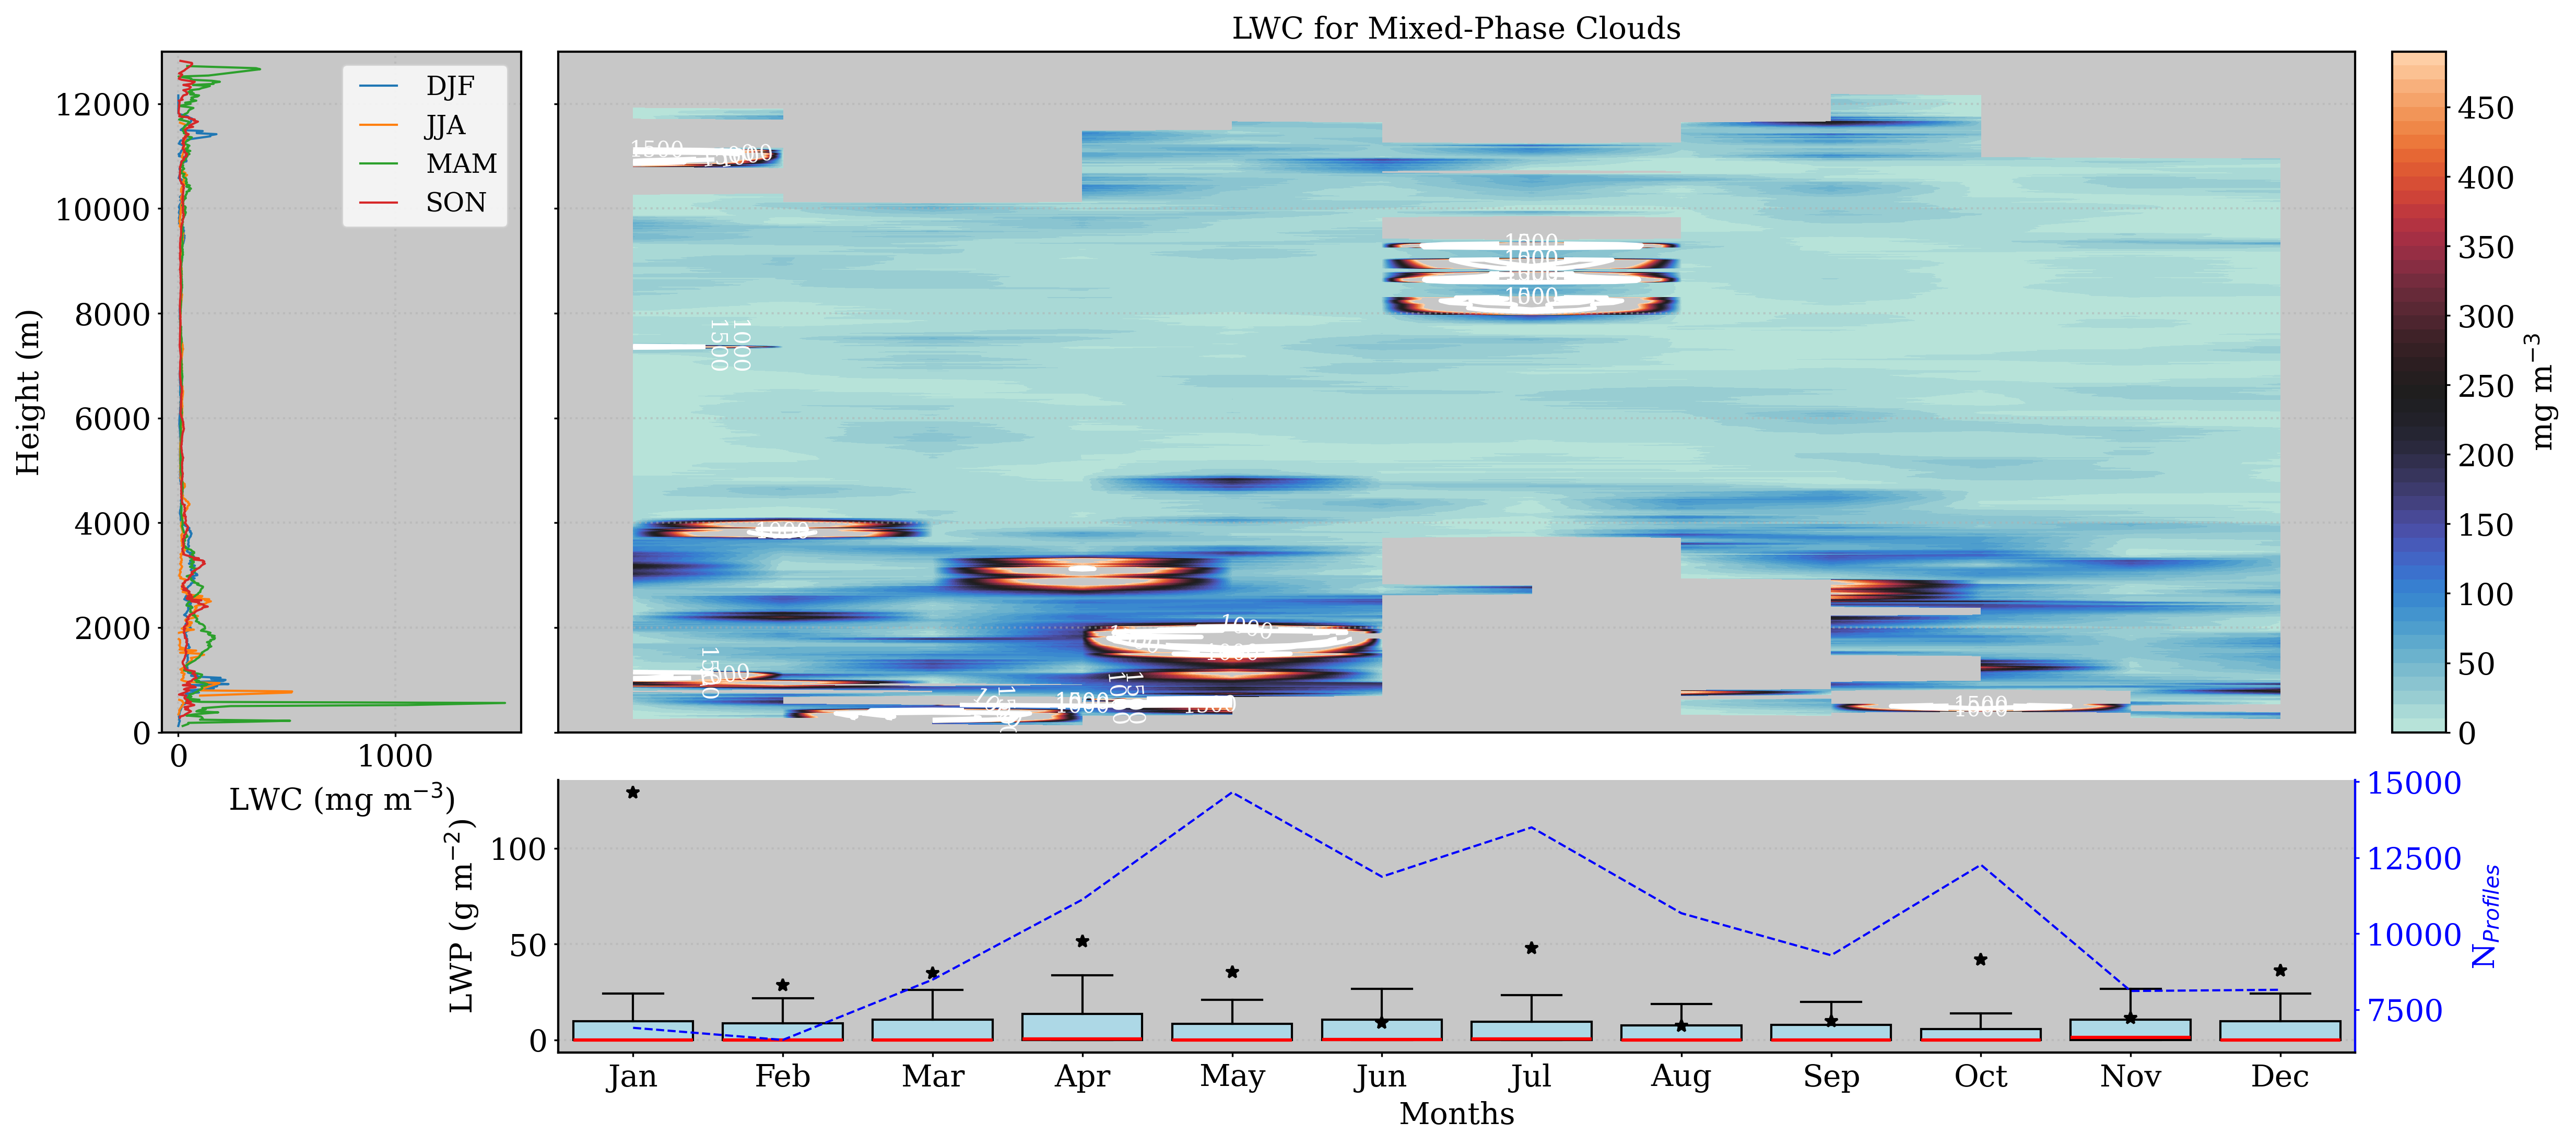
\includegraphics[width=.9\textwidth]{../../phd_clouds/figures/grouped_by_month_evolution_for_lwc_Mixed-Phase_mesh}
	\caption{Same as Figure \ref{fig:LWC_liq}, but for mixed-phase clouds.}
	\label{fig:LWC_mixed}
\end{figure}

In terms of droplet effective radius ($ r_{liq} $), a totally different nature is observed in relation to LWC. The last has expressive amounts of liquid water at low and high layers (< 4 km and > 10 km), while the first is exhibiting high droplet sizes at middle levels. Large values of droplet sizes can be observed on the right-top panel of Figure \ref{fig:DER_mixed} in dark blues and hot tones. They are normally located between 4 and 8 km throughout the entire year, except for July, which also shows larger droplets at 10 km. As already discussed, liquid water is not common at those levels, but when detected, are followed by high mass concentration, suggesting the detection of cumulus clouds. These clouds can have supercooled liquid water at high levels. 

Overall, summer presents higher droplets compared to colder months, with an effective radius between 14-22 $\mu$m at medium heights (> 4 km and < 6 km), and between 12-18$\mu$m around 10 km. On the other hand, droplet sizes are generally close to 10 $\mu$m inside these clouds. This is shown by the monthly distribution of $ r_{liq} $, where the modes are located at even smaller values than the median. In fact, cloud droplets are slightly larger in summer and have a good probability to reach 15 $\mu$m, but in general they present smaller droplets. 

In addition, there is a clear dependency of droplet size with the height. Seasonal profiles on the left panel of Figure \ref{fig:DER_mixed} show droplet size increasing up to 5 km, then starting to decrease. Thus, it is followed by all seasons, indicating that particular seasonal differences of droplet size is only grasped by monthly profile analysis. However, the seasonal profile highlights a general behavior, which can be explained by the ice particle formation. Since temperature decreases with height, ice particles will be formed, increasing the water vapor competition, stopping the process of growing of liquid droplets to form ice particles as temperature continues to decrease. These factors will decrease the size of water droplets and increase the mass concentration of ice particles. The last can be confirmed by the left panel of Figure \ref{fig:IWC_mixed}.

\begin{figure}[H]
	\centering
	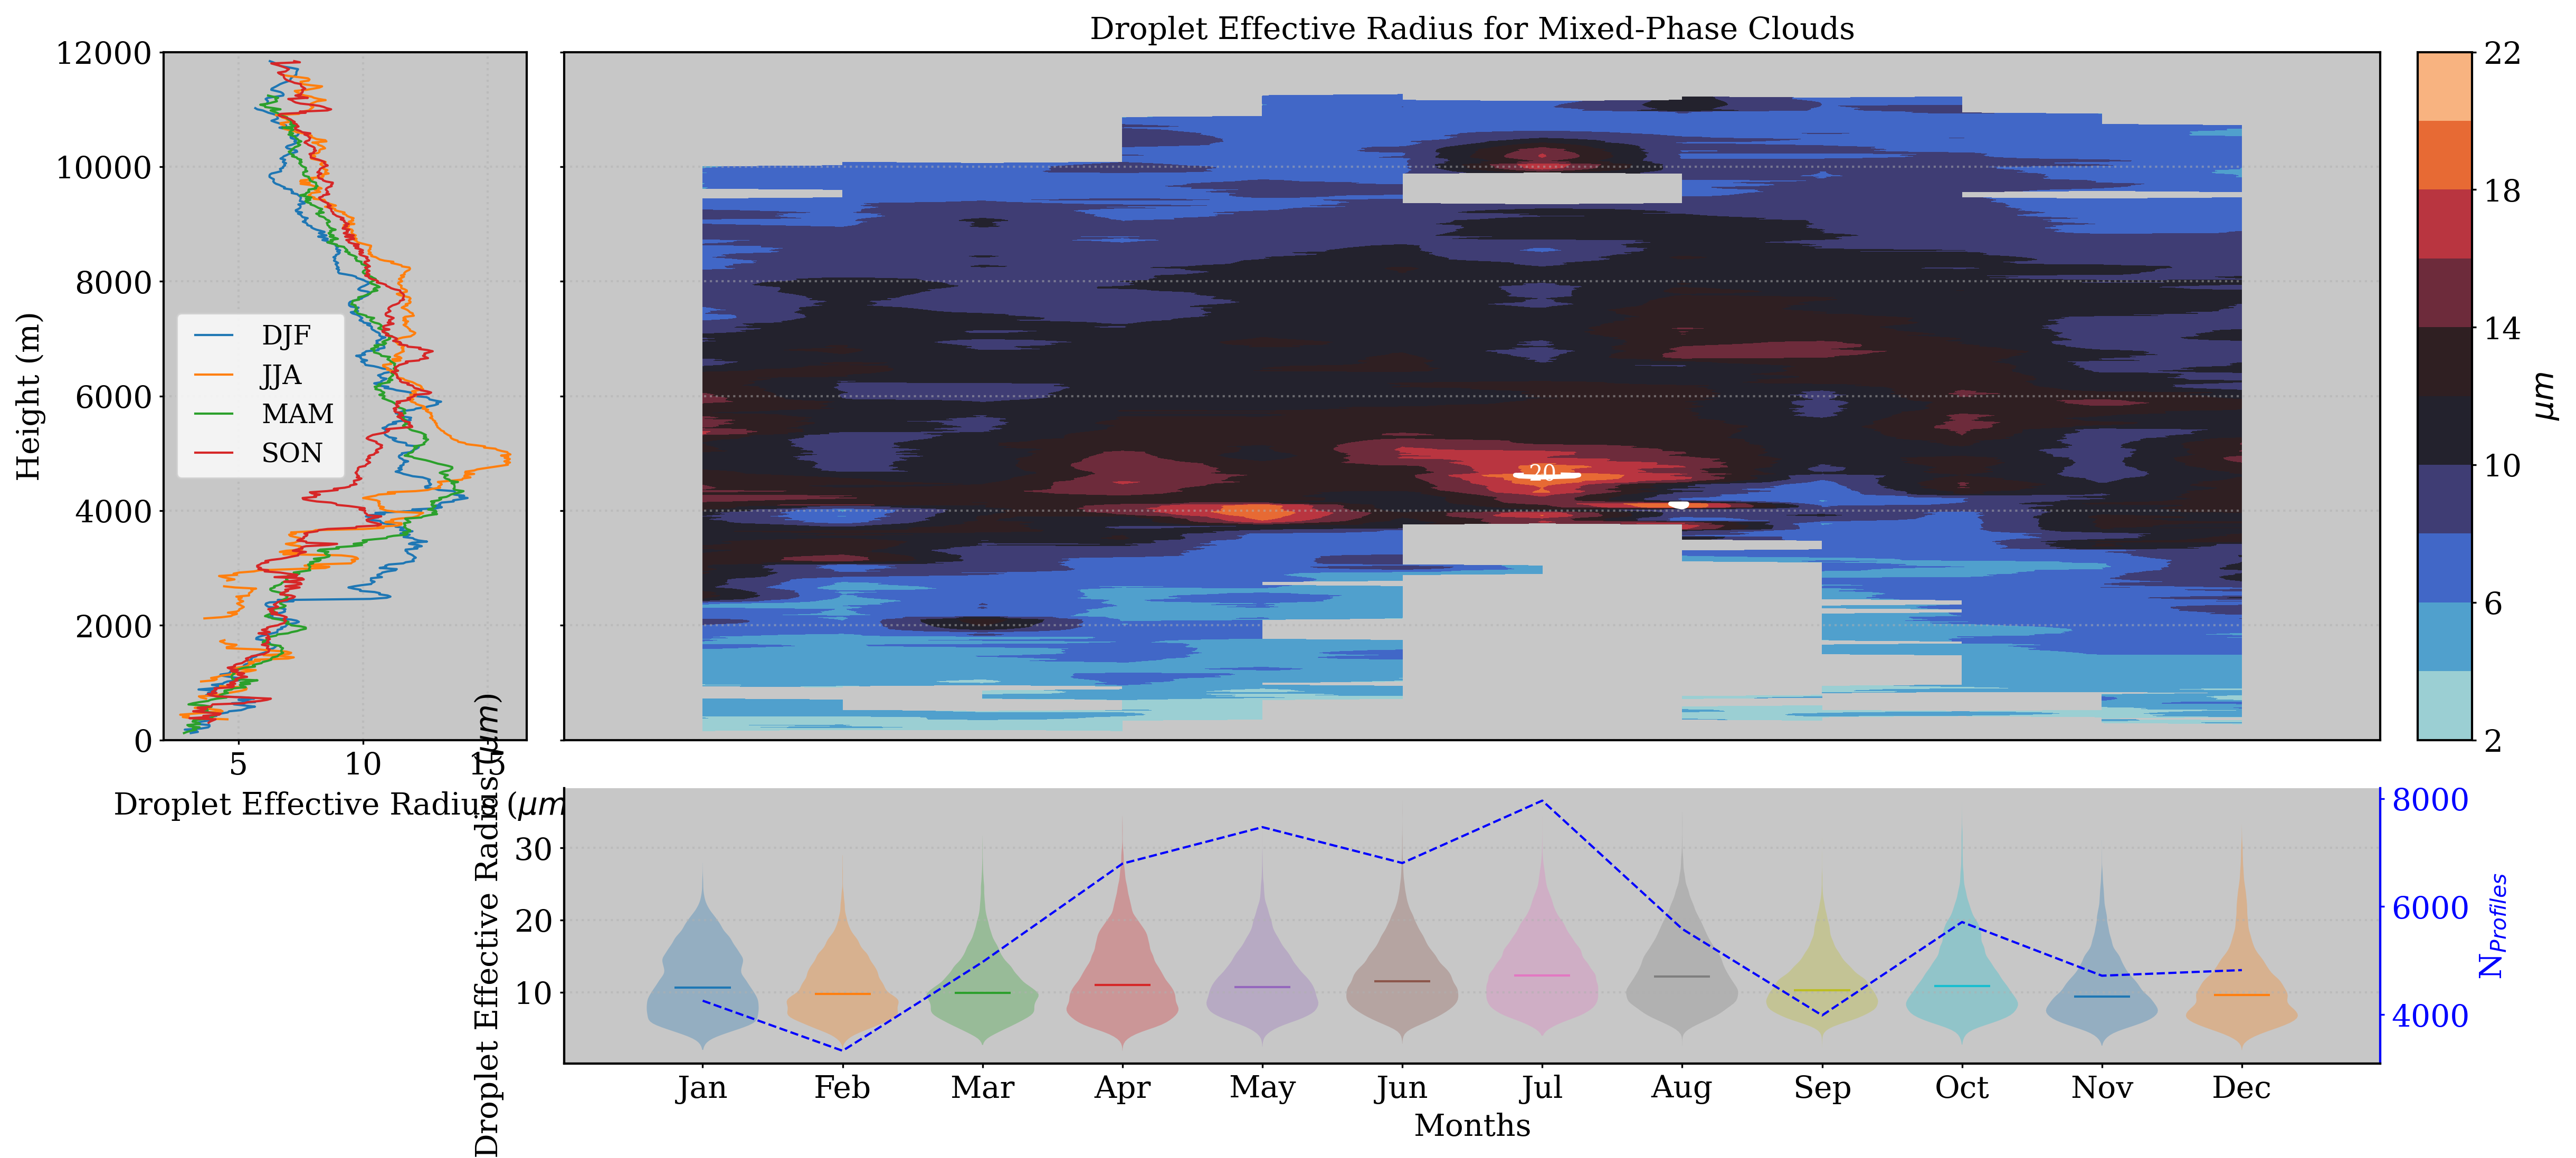
\includegraphics[width=.9\textwidth]{../../phd_clouds/figures/grouped_by_month_evolution_for_der_Mixed-Phase_mesh}
	\caption{Same as figure \ref{fig:DER_liq}, but for mixed-phase clouds.}
	\label{fig:DER_mixed}
\end{figure}

Regarding the ice water content, it exhibits significant variation with height, especially during summer. The monthly median profiles in Figure \ref{fig:IER_mixed} shows that ice mass is greater at middle/high altitudes, as expected. Normally, significant values of IWC of about 20-40 mg m$^{-3}$ are found between 4 and 10 km, except for July. As for the LWC, July also presented elevated IWC above 10 km (more than 60 mg m$^{-3}$), complementing our hypotheses that these clouds can be classified as cumulus clouds. Cumulus clouds are the first stage of cumulonimbus clouds and can have considerable amounts of ice, especially at their top.  In addition, these clouds have a considerable thickness as those observed for mixed phase clouds (some of them can reach 2 km of thickness). 

In terms of IWP, these clouds have low ice amounts as can be seen by the median in the bottom panel, normally below 10 g m$^{-2}$ throughout the entire year. However, the presence of just a few cases with high amounts of ice (outliers) can pull the average up. It happens specially in April and summer, where the physical properties of these clouds are more variable. Also, as already observed, IWC is increasing with altitude, generally formed slightly above 2 km, increasing until 7 km for colder months (winter and spring) and 8 km for warmer months (fall and summer). Winter and fall follow practically the same function of height, as well summer follows the same behavior of fall up to almost 8 km. Above this level, summer has the largest amount of IWC, with maximum, varying between 20 and 10 mg m$^{-3}$.

\begin{figure}[H]
	\centering
	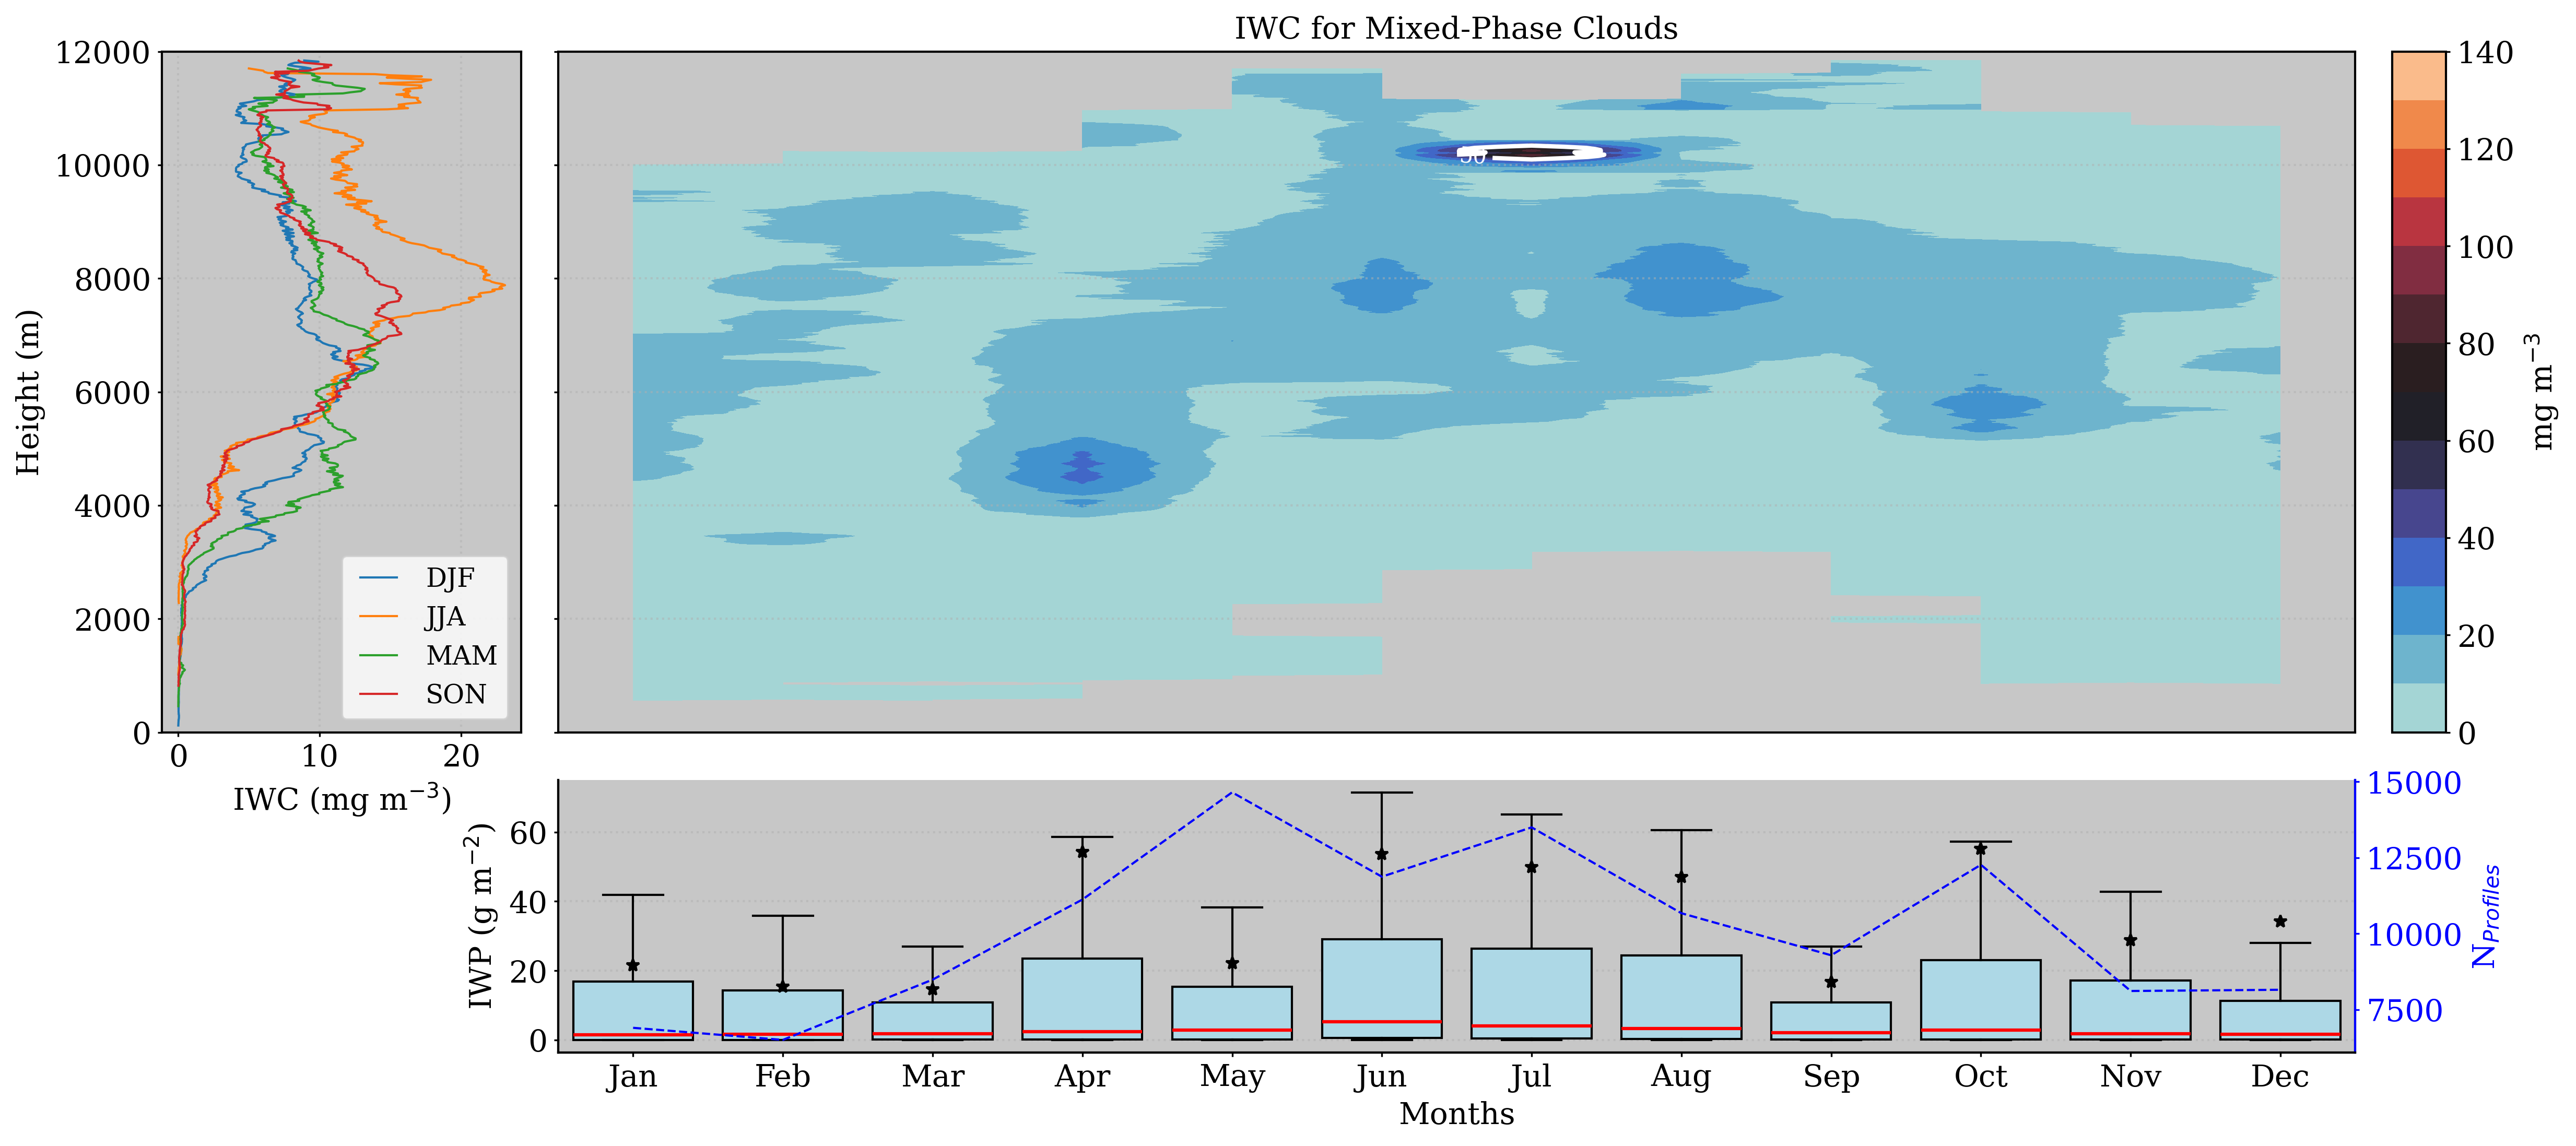
\includegraphics[width=.9\textwidth]{../../phd_clouds/figures/grouped_by_month_evolution_for_iwc_Mixed-Phase_mesh}
	\caption{Seasonal and monthly average of ice water content (IWC) and ice water path (IWP) for mixed-phase clouds. Left panel shows the seasonal median profiles of IWC. 
		%      where the shaded area indicates the standard deviation divided by 10. 
		Right panel shows the monthly median profiles of IWC and monthly box-plot of IWP in the bottom. For the boxplots, medians are denoted by red lines and the average by black stars.}
	\label{fig:IWC_mixed}
\end{figure}

In terms of effective radius, their size follows almost the inverse of the IWC in function of the height. Figure \ref{fig:IER_mixed} undoubtedly shows that higher radii are at low levels, except in July where it's possible to find $ r_{ice} $ larger than 50 $\mu$m above 10 km. Hence, the general properties of these clouds can be described as having larger ice particles with low ice water content (IWC), particularly at lower altitudes. This characteristic is not limited to summer, during which these clouds are distinctly different from those observed throughout the rest of the year. In addition, the monthly distribution (bottom panel of Figure \ref{fig:IER_mixed}) shows that larger ice effective radii are more frequent than small particles. The median is normally fluctuating around 45 $\mu$m, with the mode above this value, indicating high probability of more elevated radius. 
The seasonal profiles (on the left panel of Figure \ref{fig:IER_mixed}) also strengthened our finding that effective radius decreases with height. Actually, it is still almost constant with height up to 6 km, where it starts to decrease. Its values in summer are slightly higher but there are no significant differences over the seasons. Normally, the $ r_{ice} $ is around 30  $\mu$m above 10 km, except for July.

\begin{figure}[H]
	\centering
	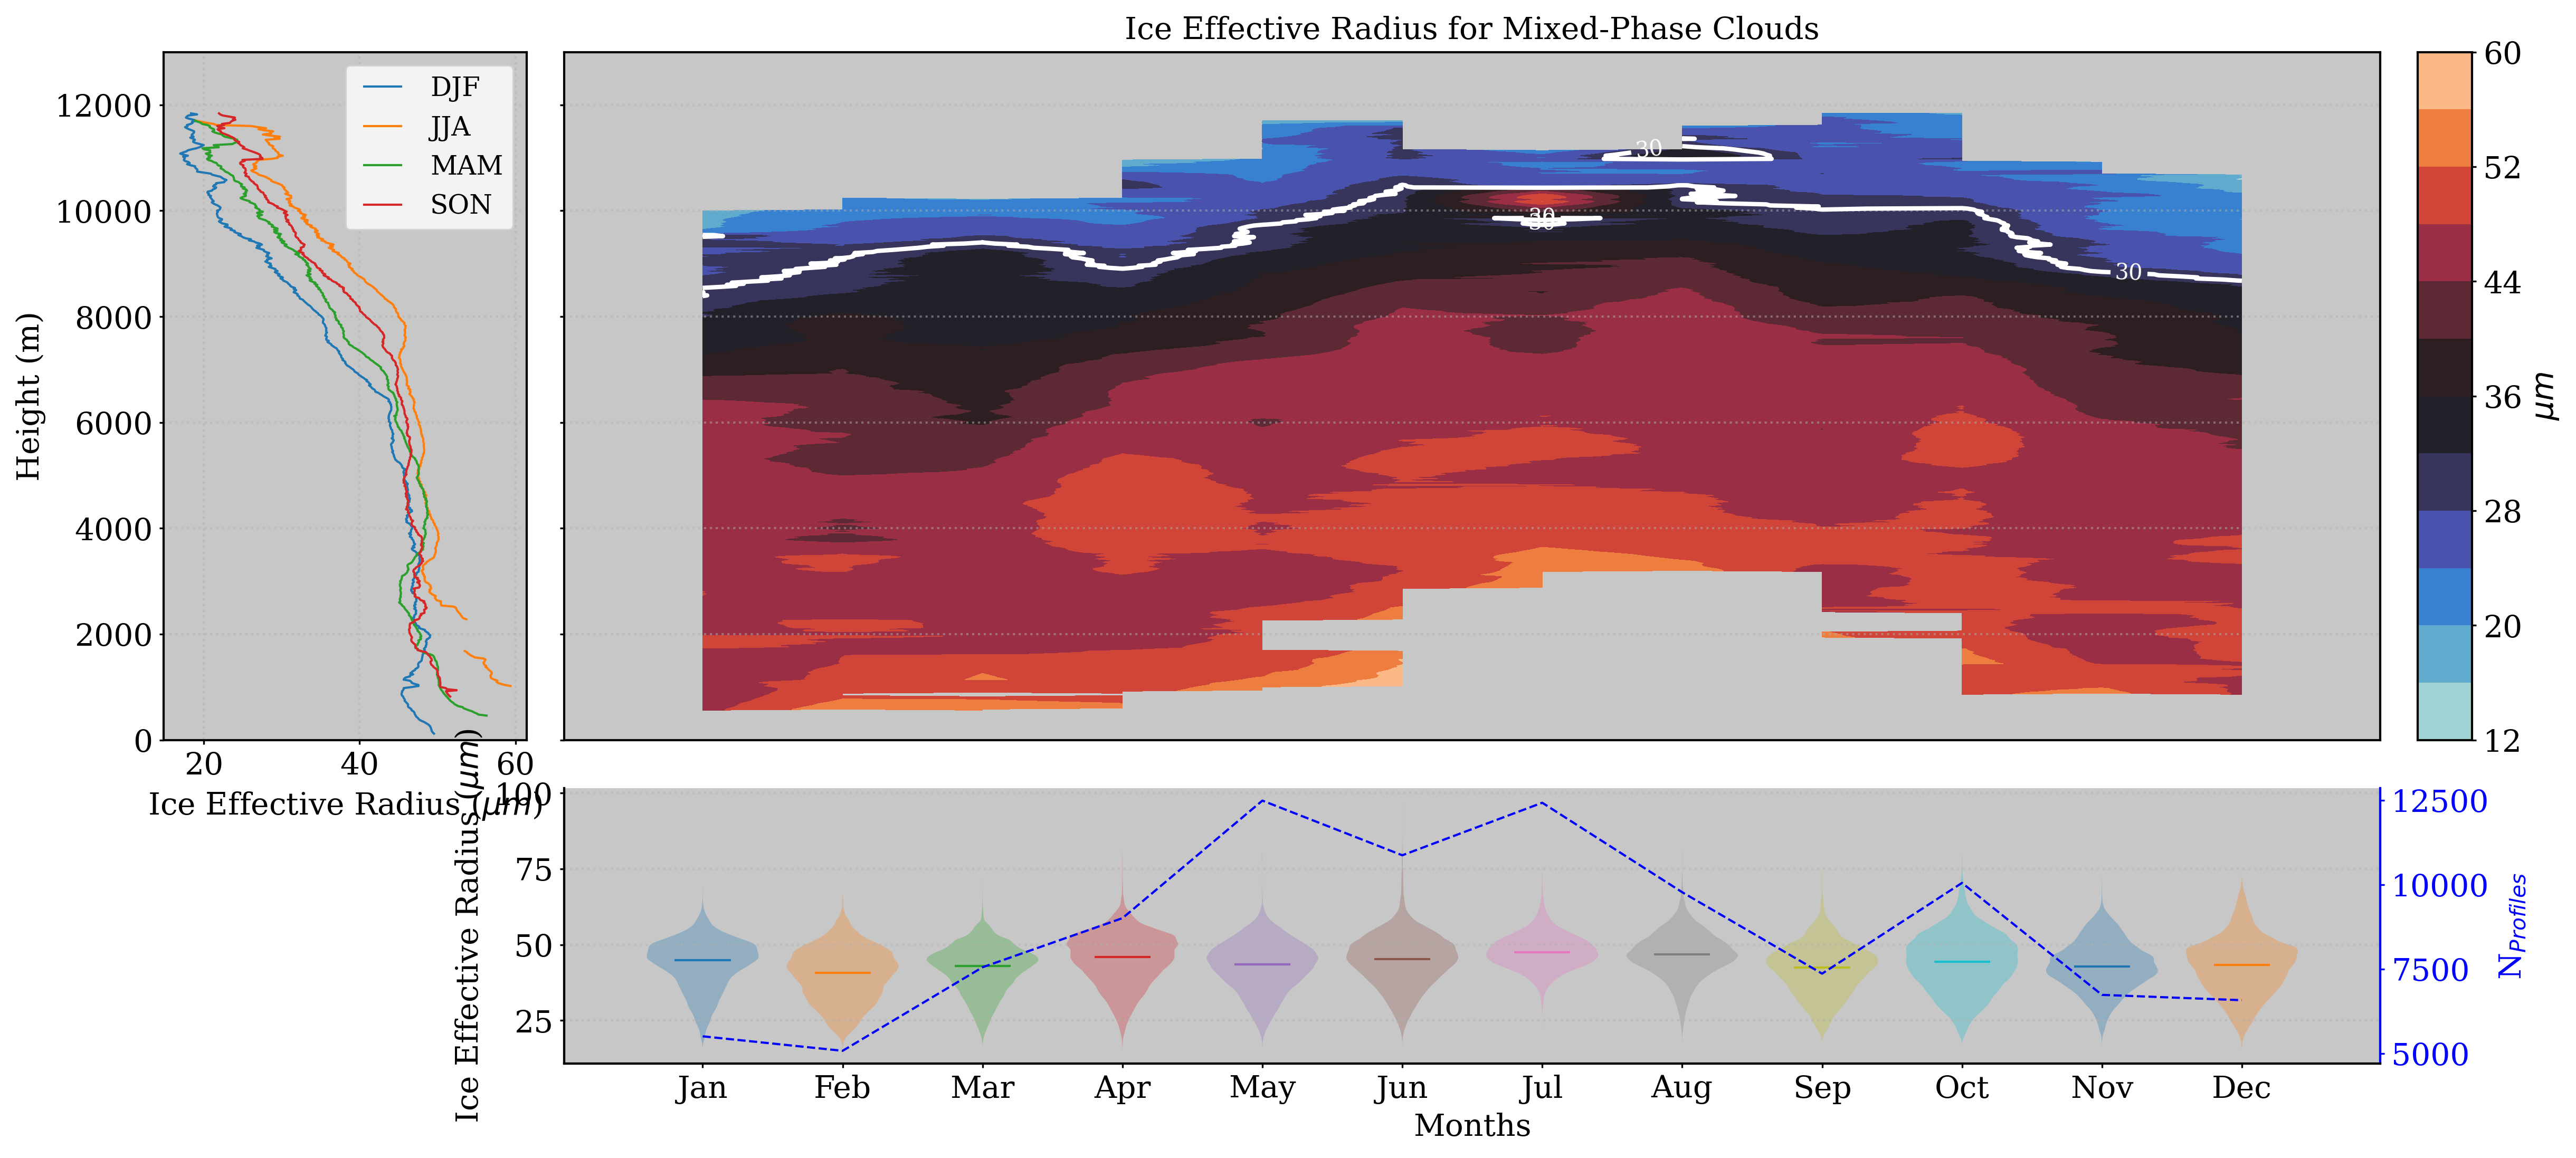
\includegraphics[width=.9\textwidth]{../../phd_clouds/figures/grouped_by_month_evolution_for_ier_Mixed-Phase_mesh}
	\caption{Seasonal and monthly statistics on ice effective radius ($r_{ice}$) distribution for mixed-phase clouds. Left panel shows the seasonal median profiles of ice effective radius. Top-right panel shows the monthly profiles of the median $r_{ice}$, while the bottom-panel displays the size distribution of $r_{ice}$ by months.}
	\label{fig:IER_mixed}
\end{figure}

Regarding the LWC, precipitating mixed-phase clouds follow a similar pattern as non precipitating clouds. However, for the precipitating case, significant amounts of liquid water are located at lower altitudes (< 4km), and they present a stronger seasonal pattern (Top-right panel of Figure \ref{fig:LWC_pre_mixed}). It is natural, considering that we already observed a strong seasonal variability in their frequency of occurrence. In addition, their liquid water content is normally higher than precipitating clouds, as expected. It is worth mentioning that the color scale in Figure \ref{fig:LWC_pre_mixed} is the same as the non precipitating case in Figure \ref{fig:LWC_mixed}, which shows much lighter areas (low values of LWC). Moreover, It is evident that these precipitating clouds do not present such high variability with height, in agreement with their cloud base distribution that showed much less variability than the non precipitating case. Following, winter and spring showed the highest values of LWC, surpassing 1000 mg m$^{-3}$ at some cases close to the surface. These periods show really sharp peaks of LWC, also observed during fall, below 1 km (see left panel). It shows that high concentrations of water in liquid phase are normally found at low levels, following the temperature pattern as expected. It is very known that the temperature at our region significantly increases in summer and fall, allowing liquid cloud droplets to be formed at higher levels. However, these months also have less humidity in the atmosphere, hindering the cloud formation as already observed by the less cloud occurrence.

For summer, a water shortage is clearly observed, especially at low levels. Both in summer and fall (hot months), considerable amounts of LWC are present at medium levels in the atmosphere (> 2 and < 4.5 km). This can be easily seen in the left panel of Figure \ref{fig:LWC_mixed}, where fall (in red) and summer (orange) have almost the same vertical profile, varying around 200 mg m$^{-3}$ between 2 and 4.5 km. At the same layer, the median profile of winter and spring goes through zero at 3 km. Furthermore, the integrated liquid water path has high variability in colder months, with medians below 50 mg m$^{-2}$ and averages above 100 mg m$^{-3}$. In summer, there are just a few occurrences of these clouds, resulting in less variability, with both medians and averages close to zero.

\begin{figure}[H]
	\centering
	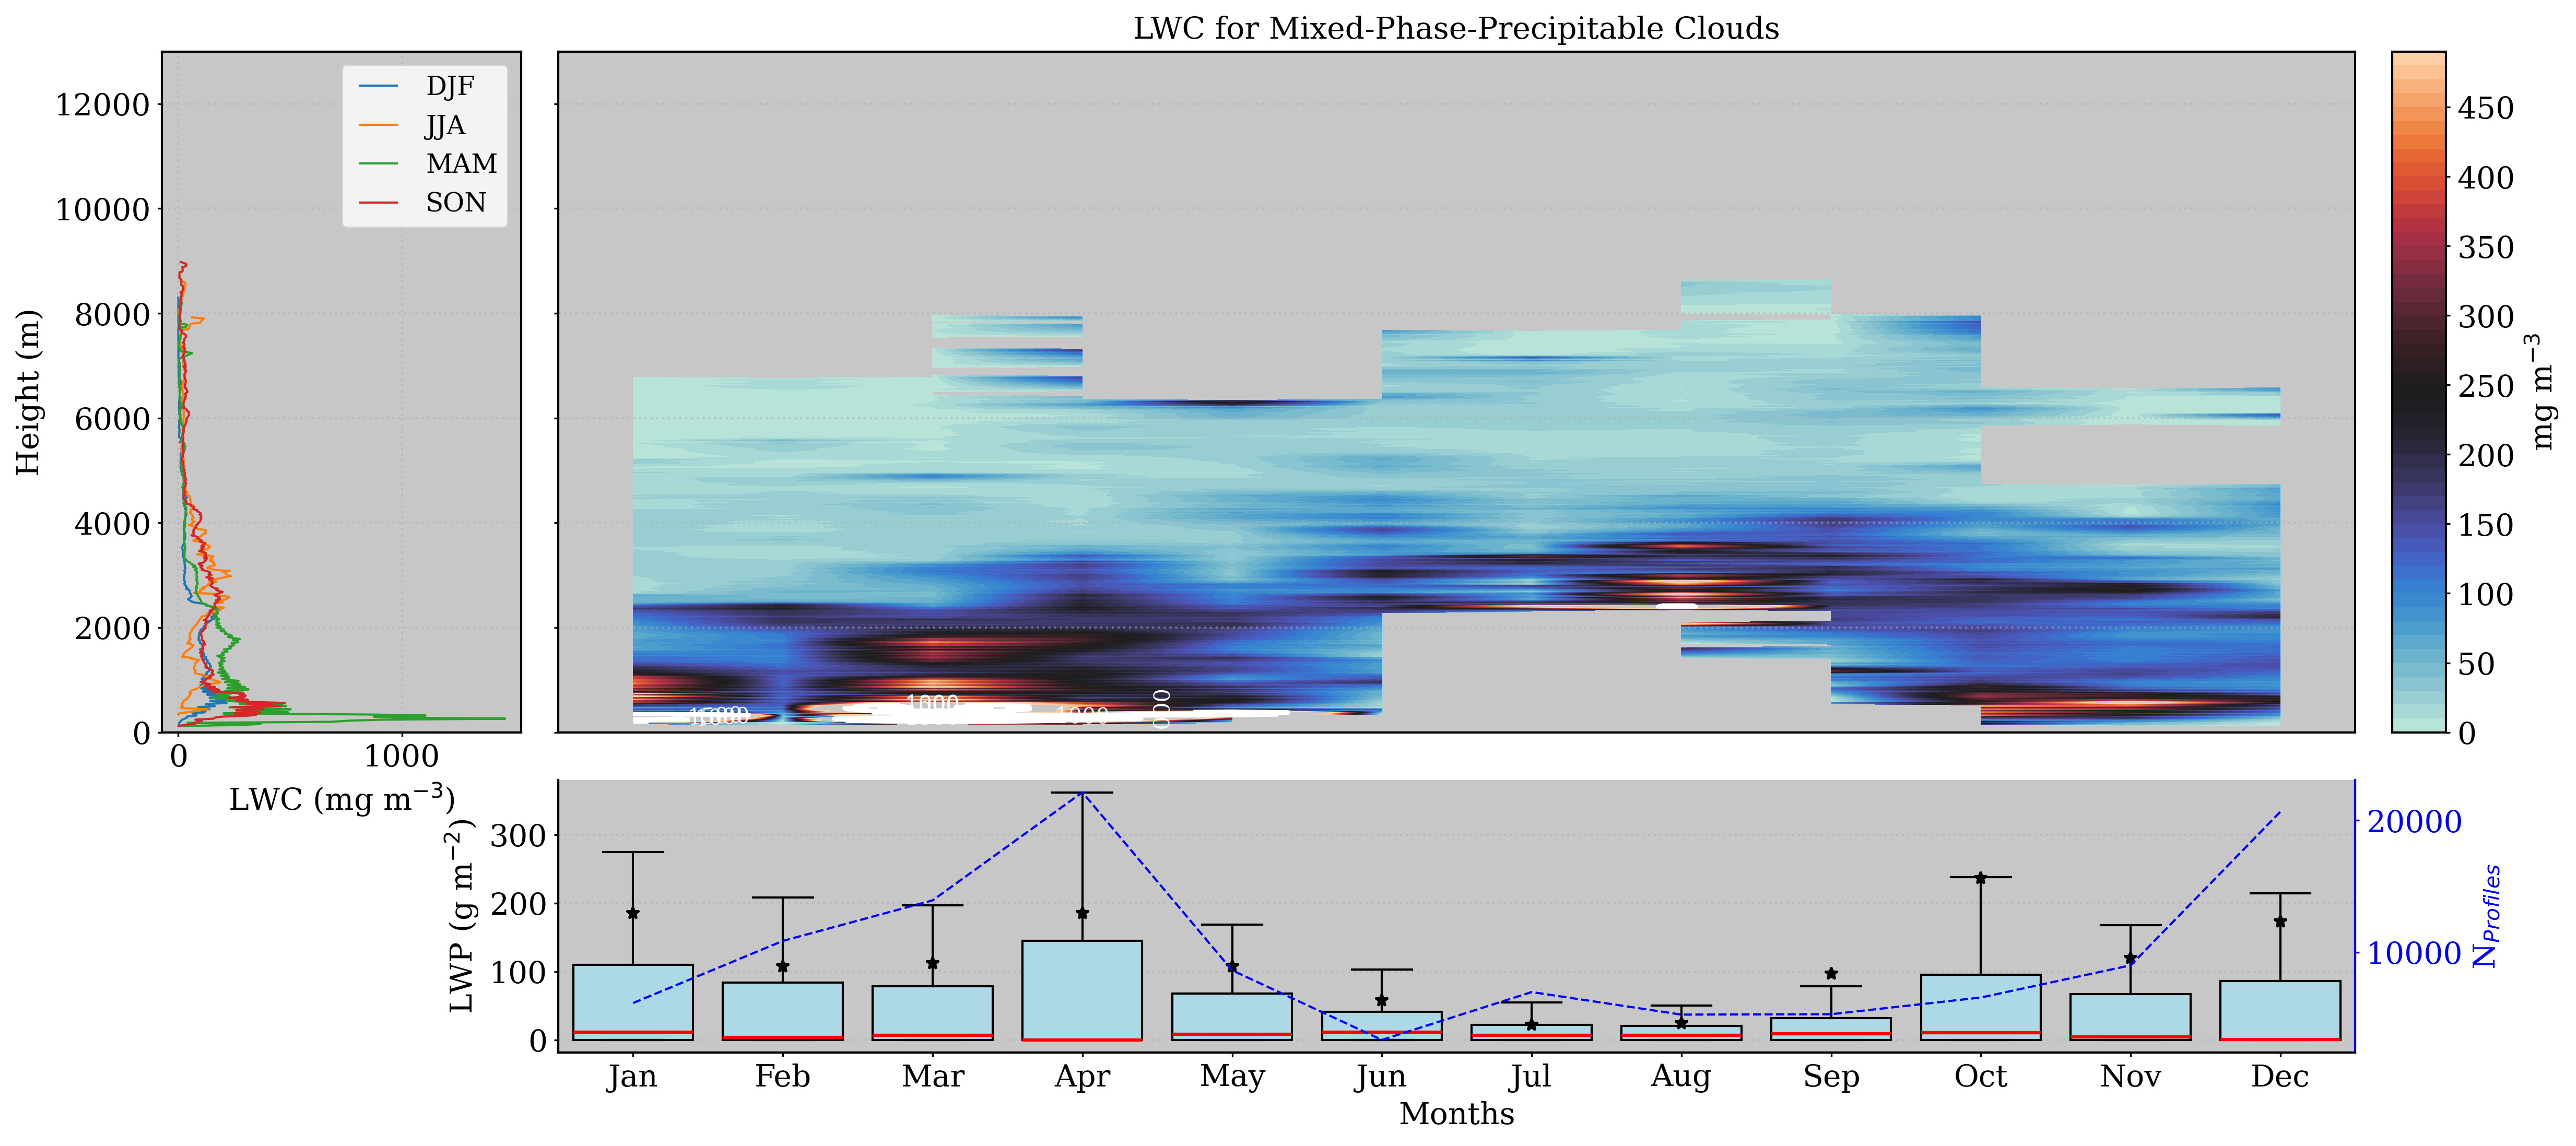
\includegraphics[width=.9\textwidth]{../../phd_clouds/figures/grouped_by_month_evolution_for_lwc_Mixed-Phase-Precipitable_mesh}
	\caption{Same as Figure \ref{fig:LWC_mixed}, but for precipitating mixed-phase clouds.}
	\label{fig:LWC_pre_mixed}
\end{figure}

In relation to the ice effective radius ($r_{ice}$), values below 8 km range from 48 to 64 $\mu$m, with slightly larger particles observed at specific heights during winter and summer—around 5 km in winter and 7 km in summer. Notably, in summer, larger ice particles of 70 $\mu$m can be identified at 10 km, coinciding with higher ice water content (IWC). Such high values can be attributed to strong convective motions, supporting the hypothesis that these summer clouds are cumulonimbus. At the same altitude, $r_{ice}$ values in other months are generally smaller than 30 $\mu$m, except in fall, which also presents higher values at 12 km. Above 1 km, particle size begins to increase (since large particles below are associated with drizzle below the cloud base). For winter and spring, $r_{ice}$ increases up to 5 km (reaching 50 $\mu$m) and then decreases to 20 and 30 $\mu$m, respectively. In contrast, for summer and fall, $r_{ice}$ increases up to 7 km (reaching 50 $\mu$m), then decreases before increasing again to reach second maxima of 50 and 63 $\mu$m, respectively. However, despite the larger variability with height, the monthly distribution of $r_{ice}$ shows a highly variable pattern with a sharp mode at the median position of 50 $\mu$m.

\begin{figure}[H]
	\centering
	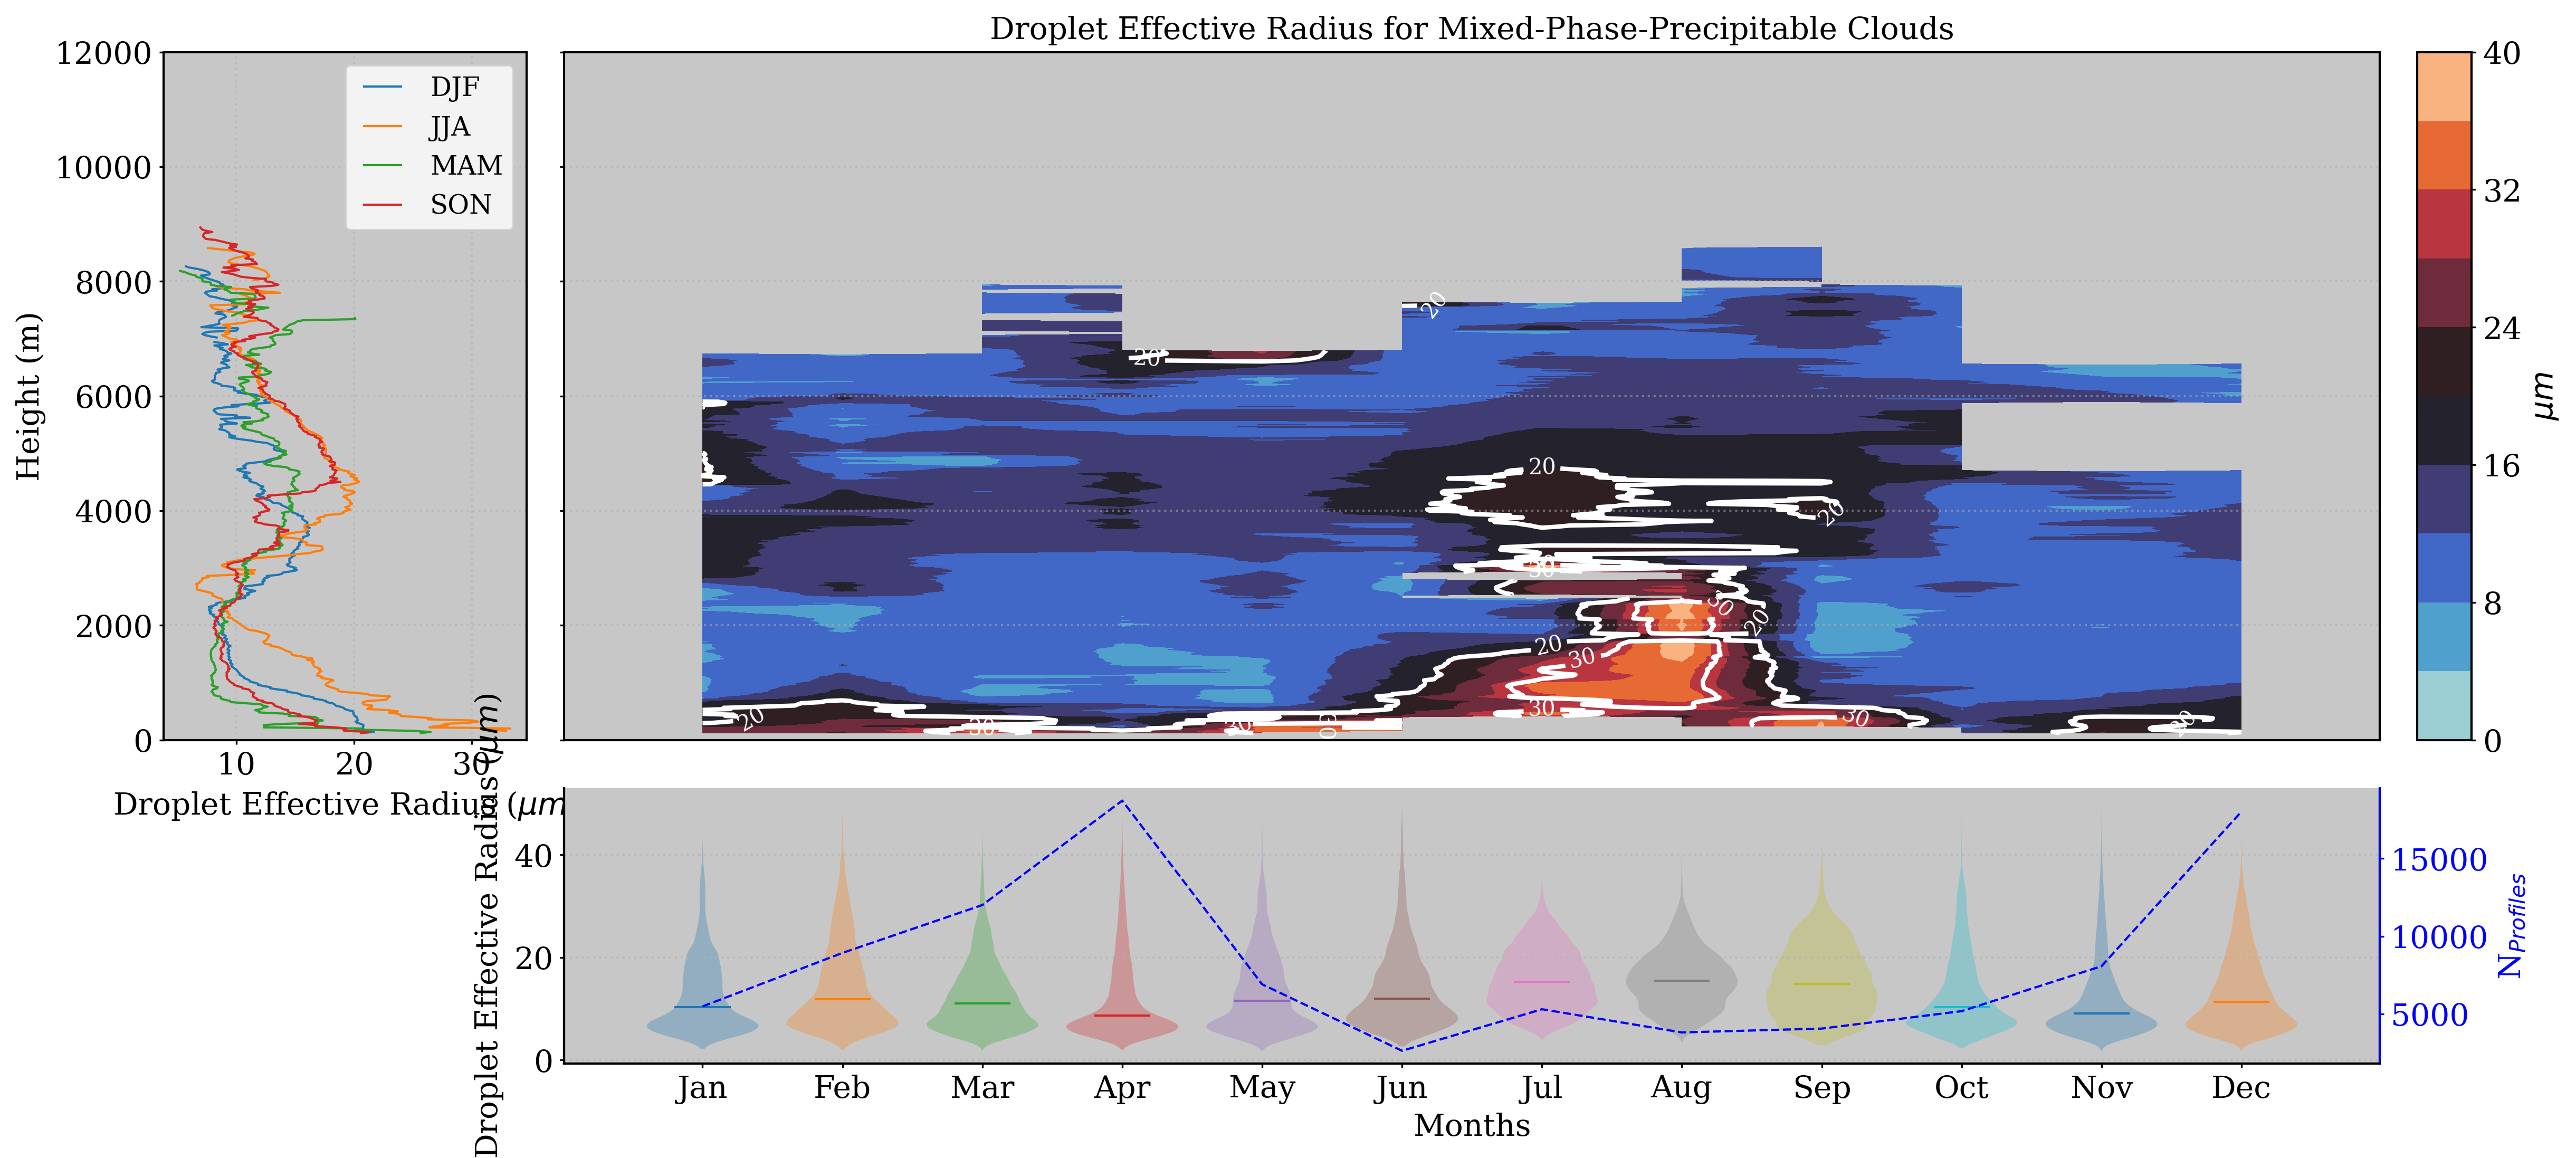
\includegraphics[width=.9\textwidth]{../../phd_clouds/figures/grouped_by_month_evolution_for_der_Mixed-Phase-Precipitable_mesh}
	\caption{Same as figure \ref{fig:DER_mixed}, but for precipitating mixed-phase clouds.}
	\label{fig:DER_pre_mixed}
\end{figure}

Following, Figure \ref{fig:IWC_pre_mixed} reveals that the ice amount inside these clouds is consistently above 3 km, exhibiting high variability with height. The largest amounts of ice water content (IWC) are found during January and November around 5 km, and in June at approximately 8-10 km. However, the median vertical profile by season (left panel of Figure \ref{fig:IWC_pre_mixed}) shows no peaks at these levels for winter, indicating that the high IWC observed in January represents particular cases rather than typical winter conditions. Typically, winter and summer IWC ranges around 20 mg m$^{-3}$ at 3.5 km and fluctuates around 5 mg m$^{-3}$ from 4 km to 9 km.
The low frequency of occurrence of these clouds in summer and fall results in comparable amounts of ice across the months, with fewer outliers. This leads to local maxima in the seasonal profiles of IWC (left panel) that align with the monthly maxima (right panel). Summer shows an almost constant IWC around 20 mg m$^{-3}$ from 5.5 to 7.5 km, with a sharp peak of 200 mg m$^{-3}$ at 9 km. Fall also exhibits IWC around 20 mg m$^{-3}$, but consistently from 5 to 9 km.
Particularly, July, August, and September have the most comparable largest amounts of IWC in the atmosphere. Consequently, the 25th, 50th, and 75th percentiles during these months are relatively higher, with 25\% of the data showing IWC values exceeding 200 mg m$^{-2}$.

\begin{figure}[H]
	\centering
	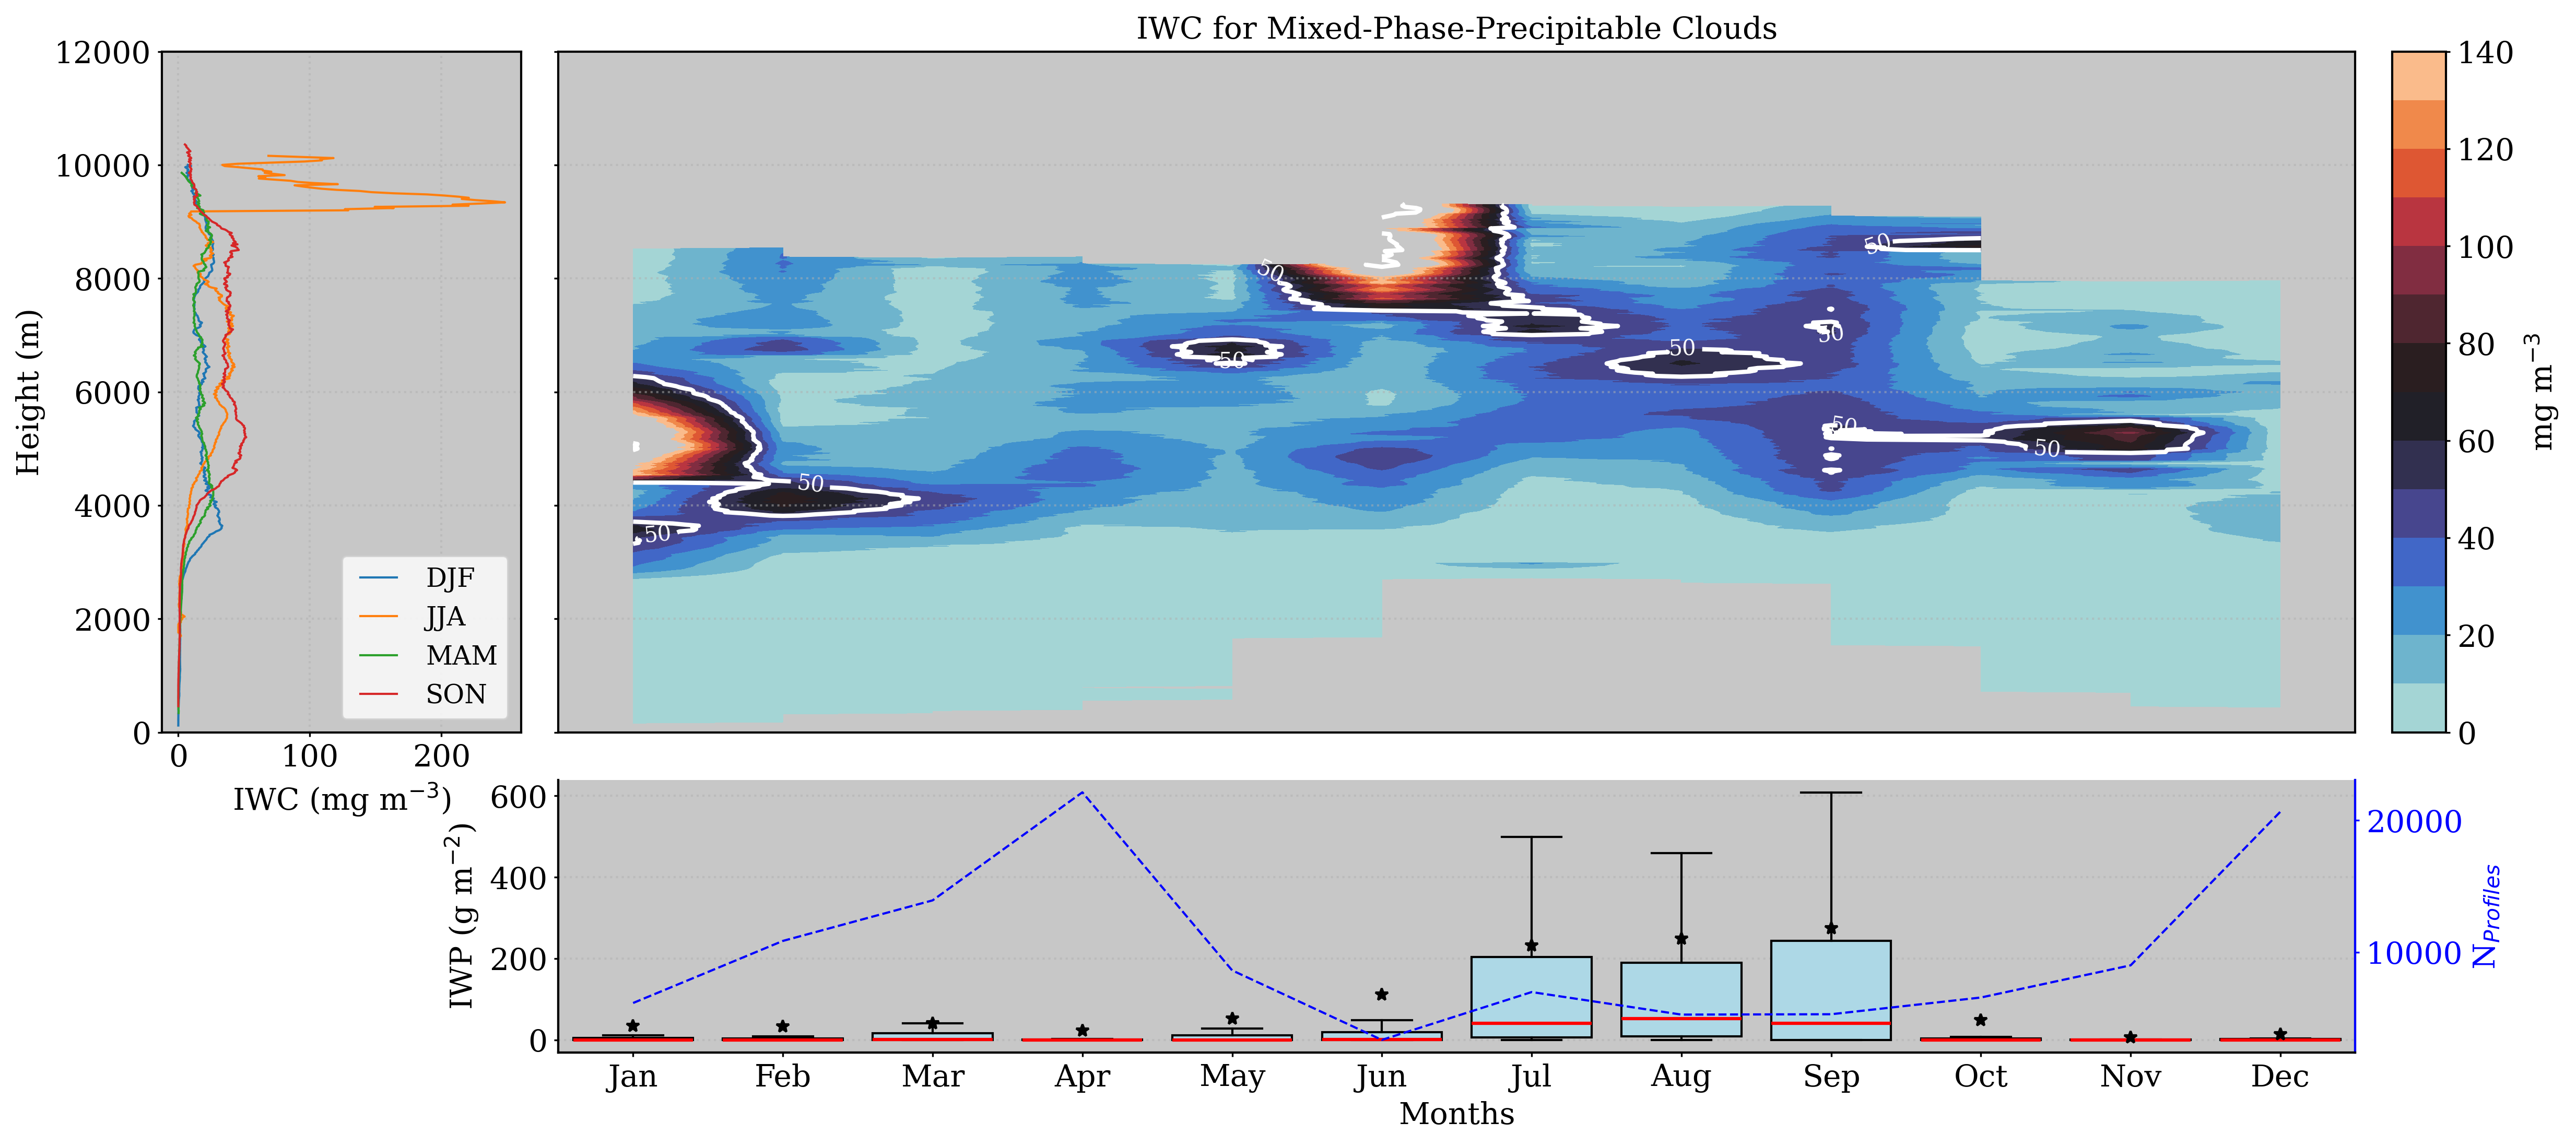
\includegraphics[width=.9\textwidth]{../../phd_clouds/figures/grouped_by_month_evolution_for_iwc_Mixed-Phase-Precipitable_mesh}
	\caption{Same as Figure \ref{fig:IWC_mixed}, but for precipitating mixed-phase clouds.}
	\label{fig:IWC_pre_mixed}
\end{figure}

In terms of effective radius, the largest values are found below 8 km, with the highest values occurring in summer and fall (dark red), as shown in Figure \ref{fig:IER_pre_mixed}. During these months, ice particle sizes exhibit less variability with height, ranging around 50-55 $\mu$m. Conversely, winter and spring show variability between 45 and 55 $\mu$m. The left panel of Figure \ref{fig:IER_pre_mixed} clearly separates warm months (summer-fall) from colder months (winter-spring).
In warm months, the ice effective radius remains almost constant around 50 $\mu$m up to 8 km. Above this altitude, particle sizes decrease in fall, while summer exhibits a sharp maximum at 9 km, coinciding with the maximum IWC region. Winter and spring also have similar $r_{ice}$ values to those in summer and fall up to 4 km, after which the sizes decrease with height, reaching 20 $\mu$m at 10 km.
Despite this variability of $r_{ice}$ with height, the monthly distribution shows that within these clouds, $r_{ice}$ is generally around 55 $\mu$m.

\begin{figure}[H]
	\centering
	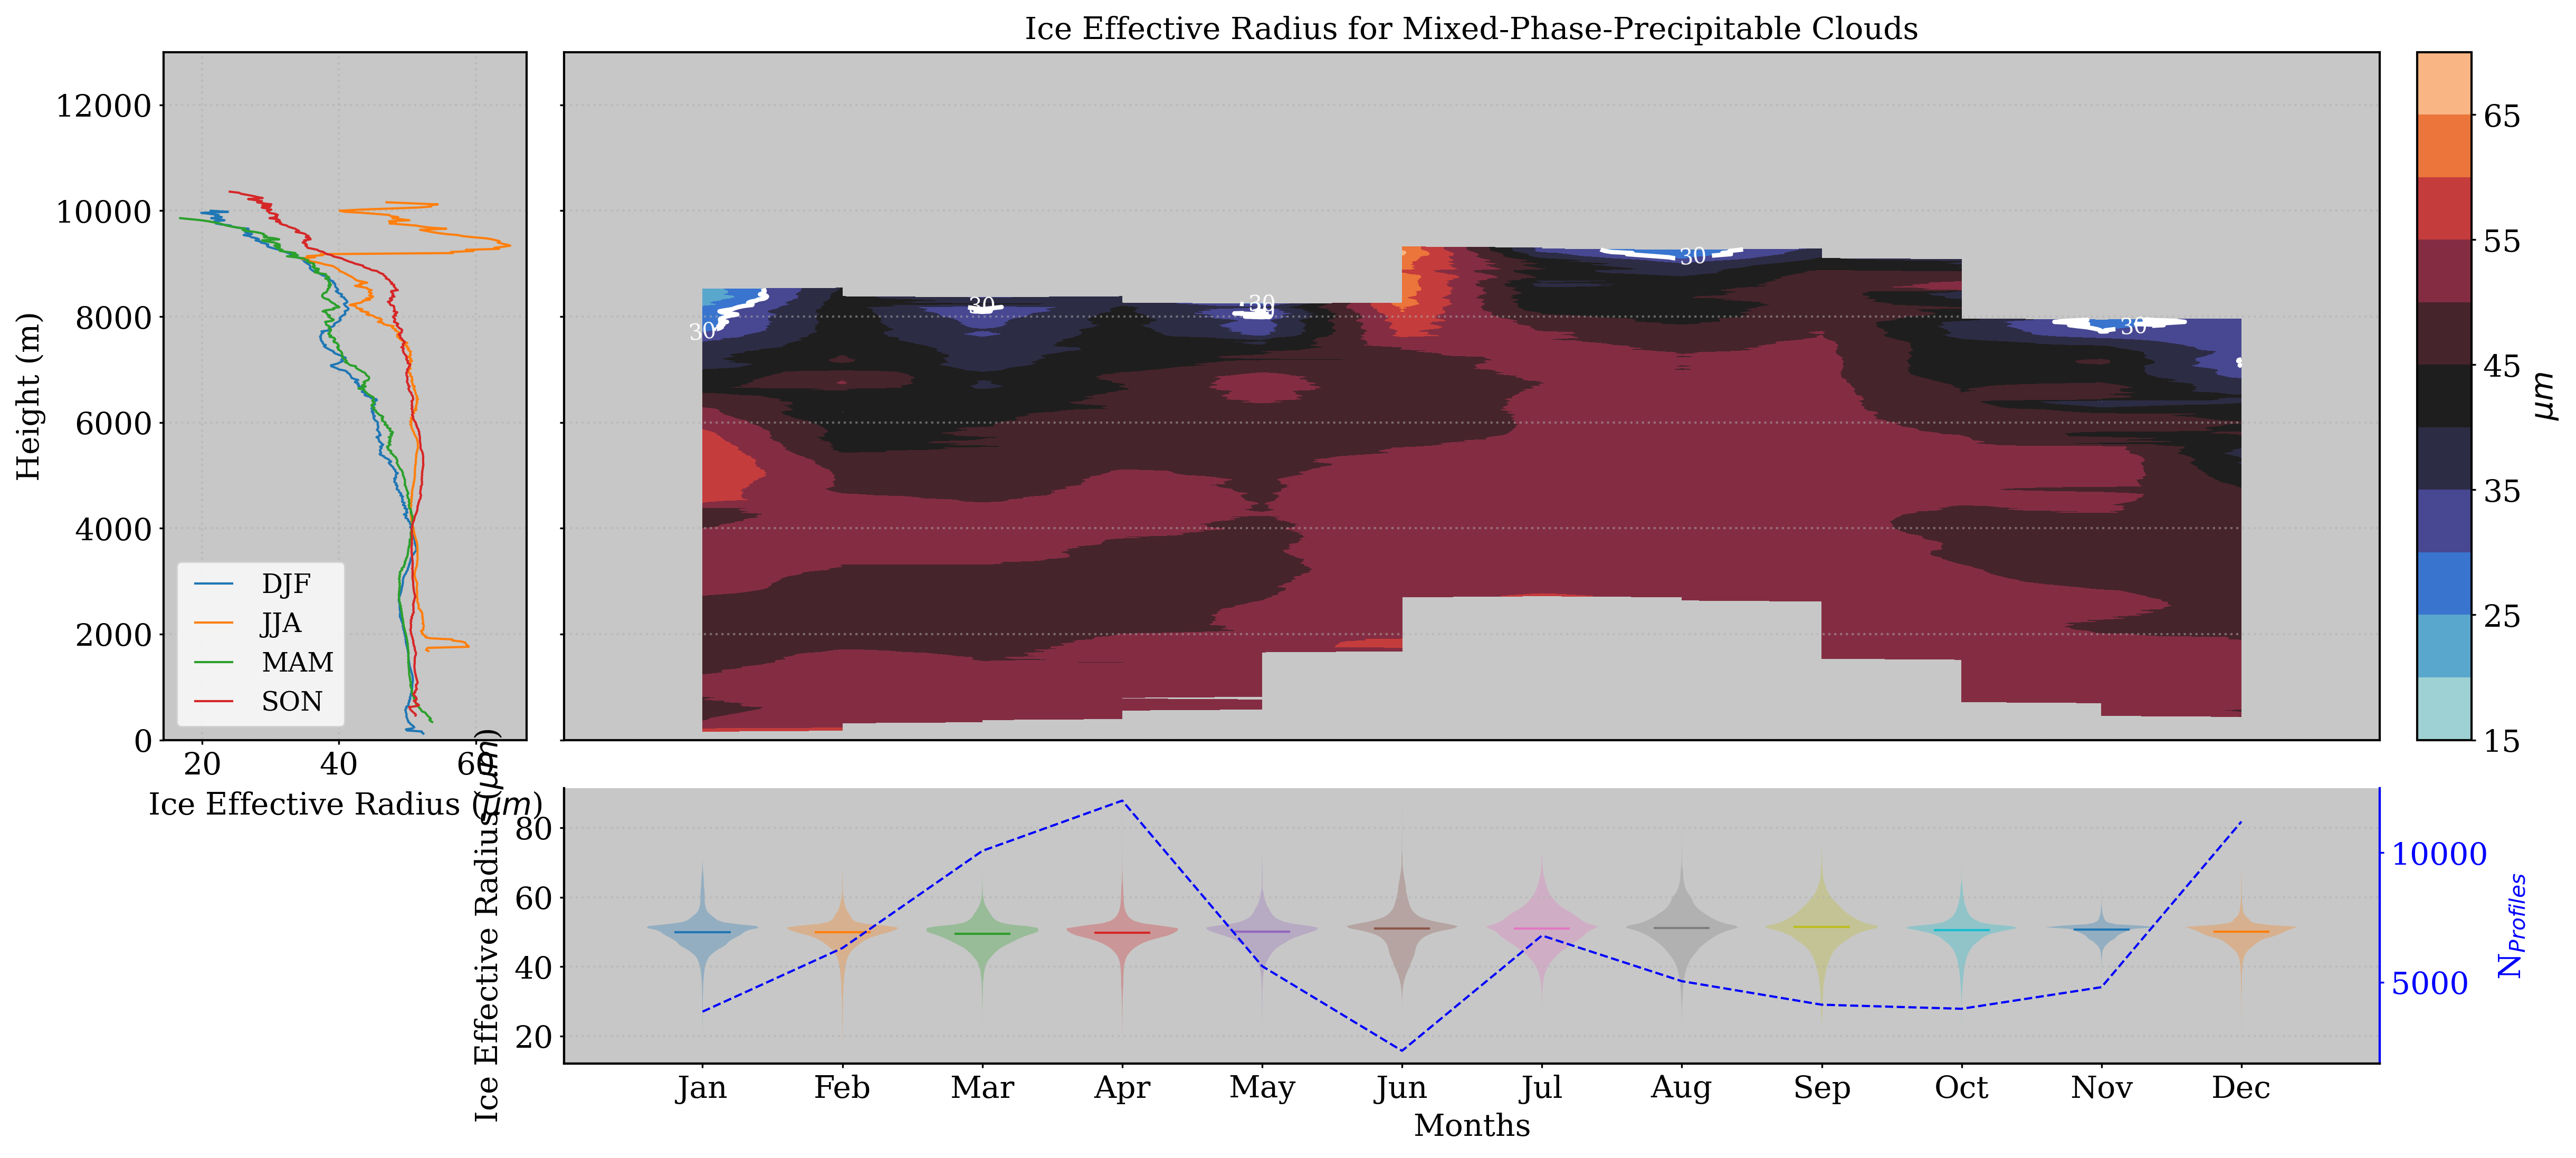
\includegraphics[width=.9\textwidth]{../../phd_clouds/figures/grouped_by_month_evolution_for_ier_Mixed-Phase-Precipitable_mesh}
	\caption{Same as figure \ref{fig:IER_mixed}, but for precipitating mixed-phase clouds.}
	\label{fig:IER_pre_mixed}
\end{figure}

Overall, Mixed-phase clouds exhibit less liquid water content (LWC) than liquid clouds. Typically, the LWC in liquid clouds is concentrated at low levels, with some exceptions in June and July, where high LWC values are observed above 8 km. Mixed-phase clouds also contain less ice water content (IWC) compared to ice clouds, with the IWC found at higher altitudes due to dependency on low temperatures, leading to elevated IWC levels higher in the atmosphere during summer. The droplet effective radius in mixed-phase clouds is larger at mid-levels, while the ice effective radius is larger at mid-levels during winter and spring and around 8 km during fall and summer. Unlike this pattern, the ice effective radius in these clouds slightly decreases with height up to 6 km, where the rate of decrease intensifies. Precipitating mixed-phase clouds exhibit a stronger seasonal profile, with higher LWC, particularly in spring and fall at lower levels. They also show significantly more IWC in summer and early fall. The droplet effective radius ($r_{liq}$) in precipitating mixed-phase clouds is typically higher than in mixed-phase clouds, especially near the surface and at mid-levels, due to the presence of drizzle particles at low levels. In terms of the ice effective radius ($r_{ice}$), these clouds display a clear seasonal variation, with higher $r_{ice}$ values in summer and fall above 4 km. Additionally, precipitating clouds show larger IWC and $r_{ice}$ values at 9 km in summer, suggesting a possible association with cumulus clouds.


\subsubsection{Ice Clouds}

The ice water content (IWC) of ice clouds exhibits clear seasonal patterns, as evident from Figure \ref{fig:IWC_ice}. The smallest ice amounts are observed in summer, particularly in July, coinciding with the minimum frequency of ice cloud occurrence. In contrast, the highest IWC values, exceeding 50 mg m$^{-3}$, are found at altitudes of 4-6 km in June and October, and near the ground in January. Typically, these clouds are situated higher in the atmosphere, with cloud bases around 7-8 km, with only 25\% of ice clouds having bases below 6 km. These lower clouds generally contain the largest ice amounts, ranging between 30 and 100 mg m$^{-3}$, except in January. Notably, January exhibits much higher IWC near the ground, an anomaly attributed to extreme weather events such as the Filomena storm in 2020 and the Gloria storm in 2021, which significantly impacted the western Mediterranean region \citep{samuelt.buisanAdjustmentSolidPrecipitation2022,mariaeugeniaperez-gonzalezEvaluationImpactCaused2022,martadealfonsoStormGloriaSea2021}. Conversely, clouds above 8 km, often associated with cirrus clouds, typically have much lower ice content, ranging from 0 to 20 mg m$^{-3}$, except in fall, where clouds with IWC around 50 mg m$^{-3}$ are observed at 12 km. These seasonal variations are also evident in the left panel of Figure \ref{fig:IWC_ice}, which shows substantial ice near the surface in winter. This was already identified as the influence of  two snowfall events, resulting in a median IWC of 400 mg m$^{-3}$ around 1 km. The variability compared to other years without such high IWC values is highlighted in the bottom panel of Figure \ref{fig:IWC_ice}, where the average liquid water path (LWP) is much higher than the median for January, indicating that typical IWP values for January are low, around 10 mg m$^{-2}$. Overall, the monthly IWP distributions for ice clouds are relatively consistent throughout the year, indicating a well-defined annual IWP pattern, except in January and July. January shows lower occurrence rates and is impacted by the snowfall events, while July is characterized by an extremely low occurrence of ice clouds, resulting in a minimum LWP.

\begin{figure}[H]
	\centering
	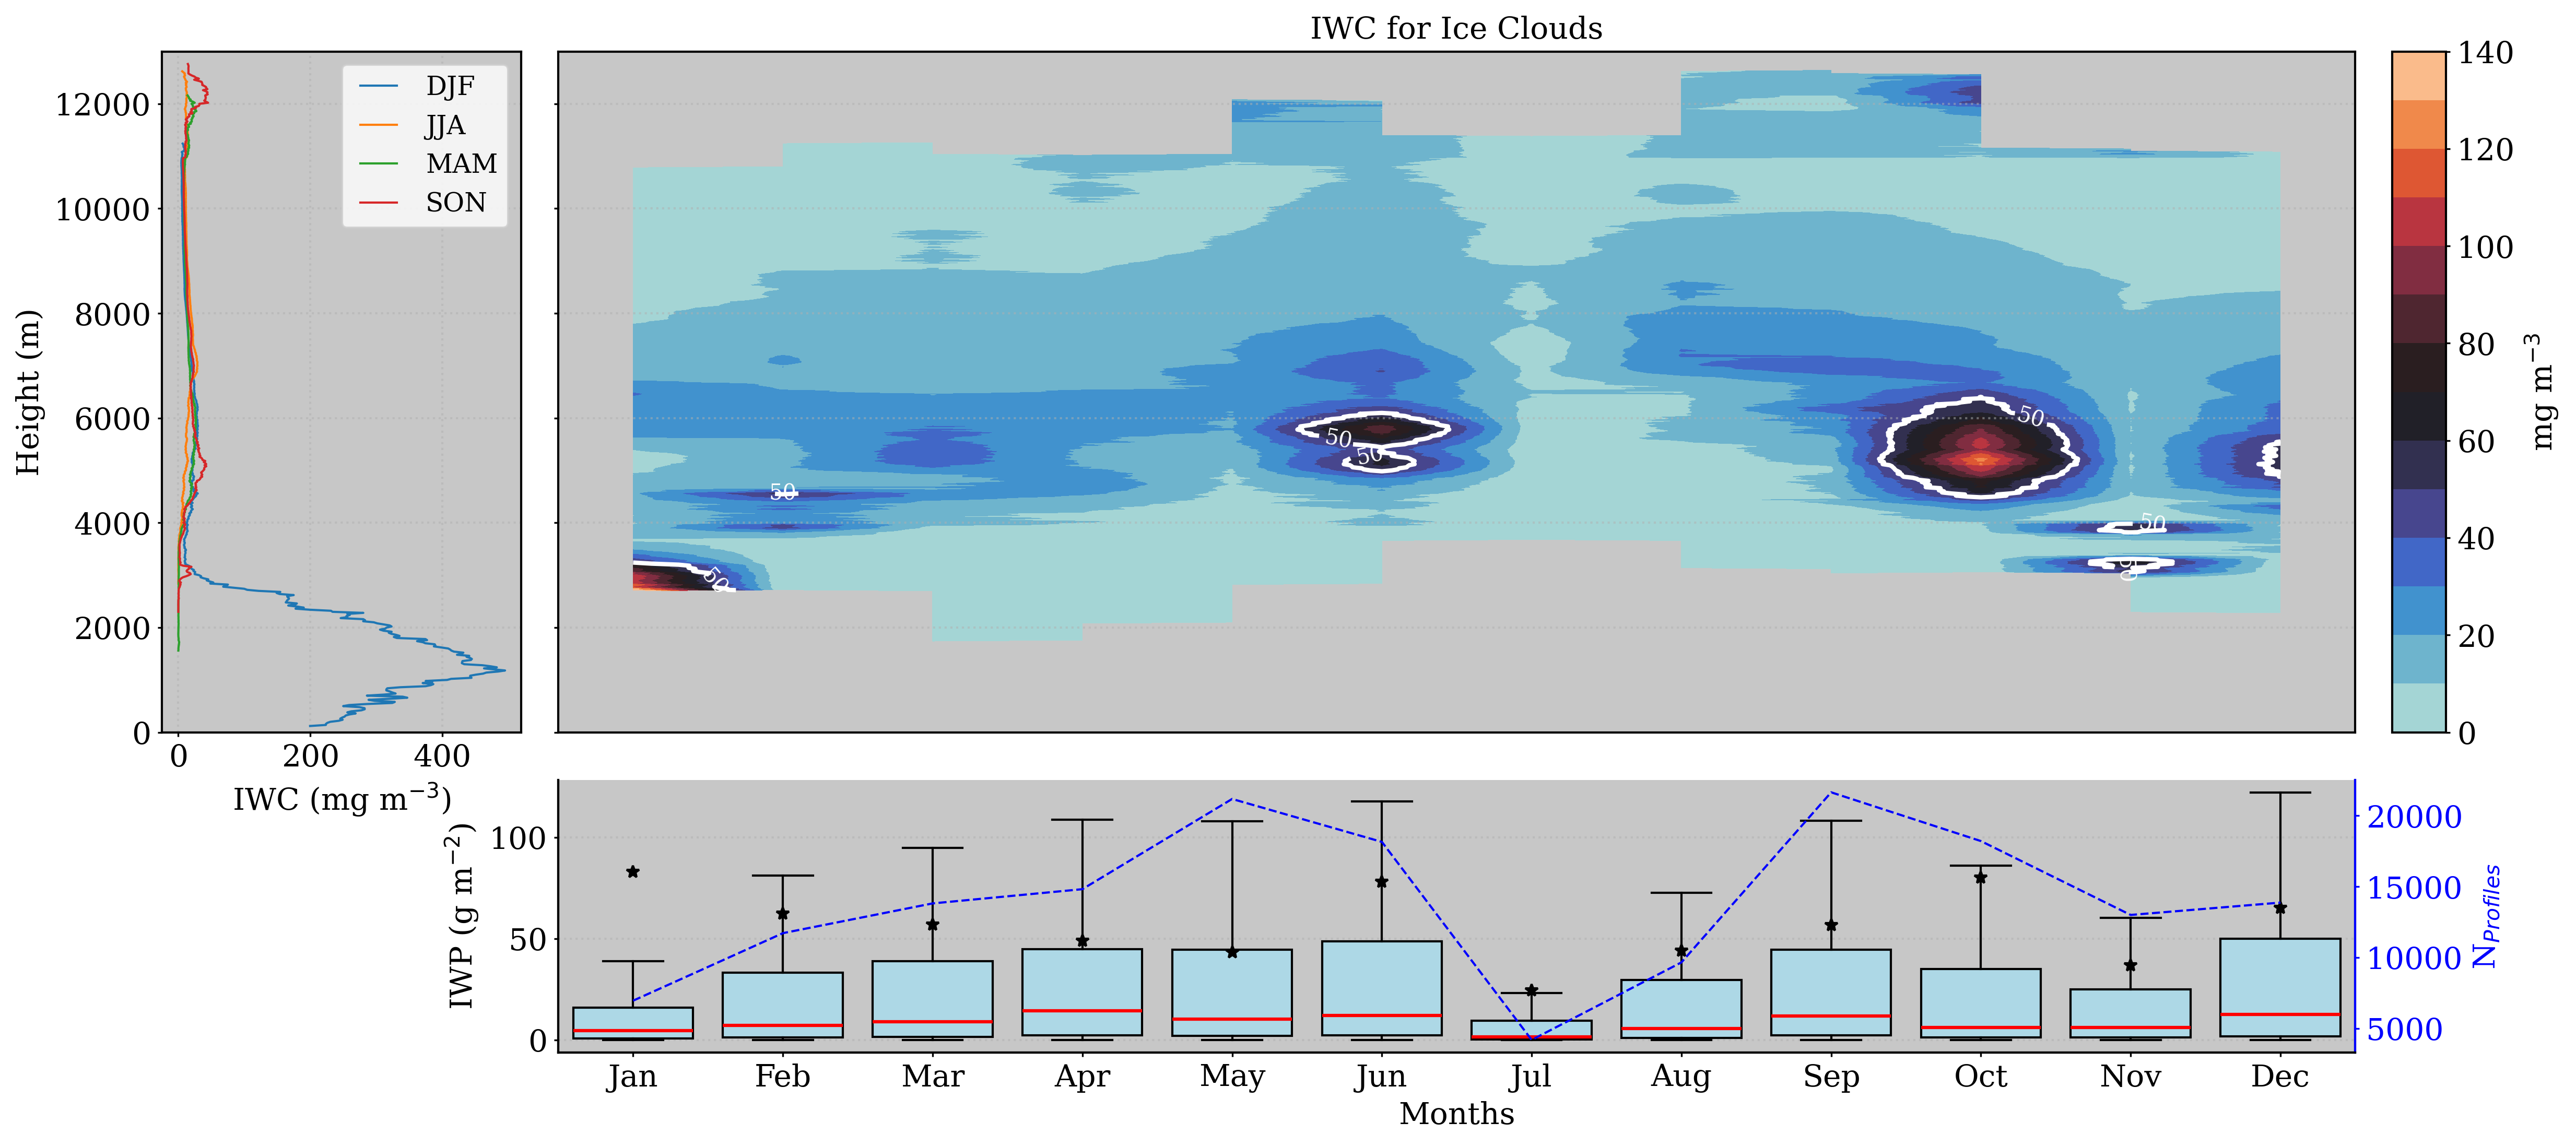
\includegraphics[width=.9\textwidth]{../../phd_clouds/figures/grouped_by_month_evolution_for_iwc_Ice_mesh}
	\caption{Seasonal and monthly average of ice water content (IWC) and ice water path (IWP) for ice clouds. Left panel shows the seasonal median profiles of IWC. 
		%      where the shaded area indicates the standard deviation divided by 10. 
		Right panel shows the monthly median profiles of IWC and monthly box-plot of IWP in the bottom. For the boxplots, medians are denoted by red lines and the average by black stars.}
	\label{fig:IWC_ice}
\end{figure}

In terms of ice effective radius, their size is also larger at middle levels, ranging around 50 and 60 $\mu$m. In addition, January also presented elevated $r_{ice}$ closer to the ground (clearly seen in the left panel of figure Figure \ref{fig:IER_ice}), as a result of the snowfalls. However, beyond this month, the maximum size of 60 $\mu$m is normally observed exclusively in June and October in mid levels. Left panel of Figure \ref{fig:IER_ice} shows that above 6 km, ice particle size diminishes, indicating a larger cloud radius at lower levels, a pattern also observed in mixed-phase clouds. Typically, ice particles are larger at low and mid-levels, except in clouds with significant convective activity, such as cumulus and cumulonimbus clouds. Cirrus clouds situated above 8 km have an ice effective radius between 40 and 45 $\mu$m, decreasing with altitude up to 11 km. At this level, during spring and summer, these clouds reach 25 $\mu$m, while in winter, the size reduces to 20 $\mu$m (see Left panel of Figure \ref{fig:IER_ice}). In fall, a slight increase in size is observed at 12 km, coinciding with high IWC levels, linked to cirrus clouds with higher ice crystal concentrations. The monthly distribution reveals a stable median ice particle size of approximately 38 $\mu$m throughout the year, indicating that this value is generally representative when considering all radii within the atmosphere for this cloud type. However, January presents a distribution with a new mode around 50 $\mu$m, as expected due to the snowfall events already discussed. 

\begin{figure}[H]
	\centering
	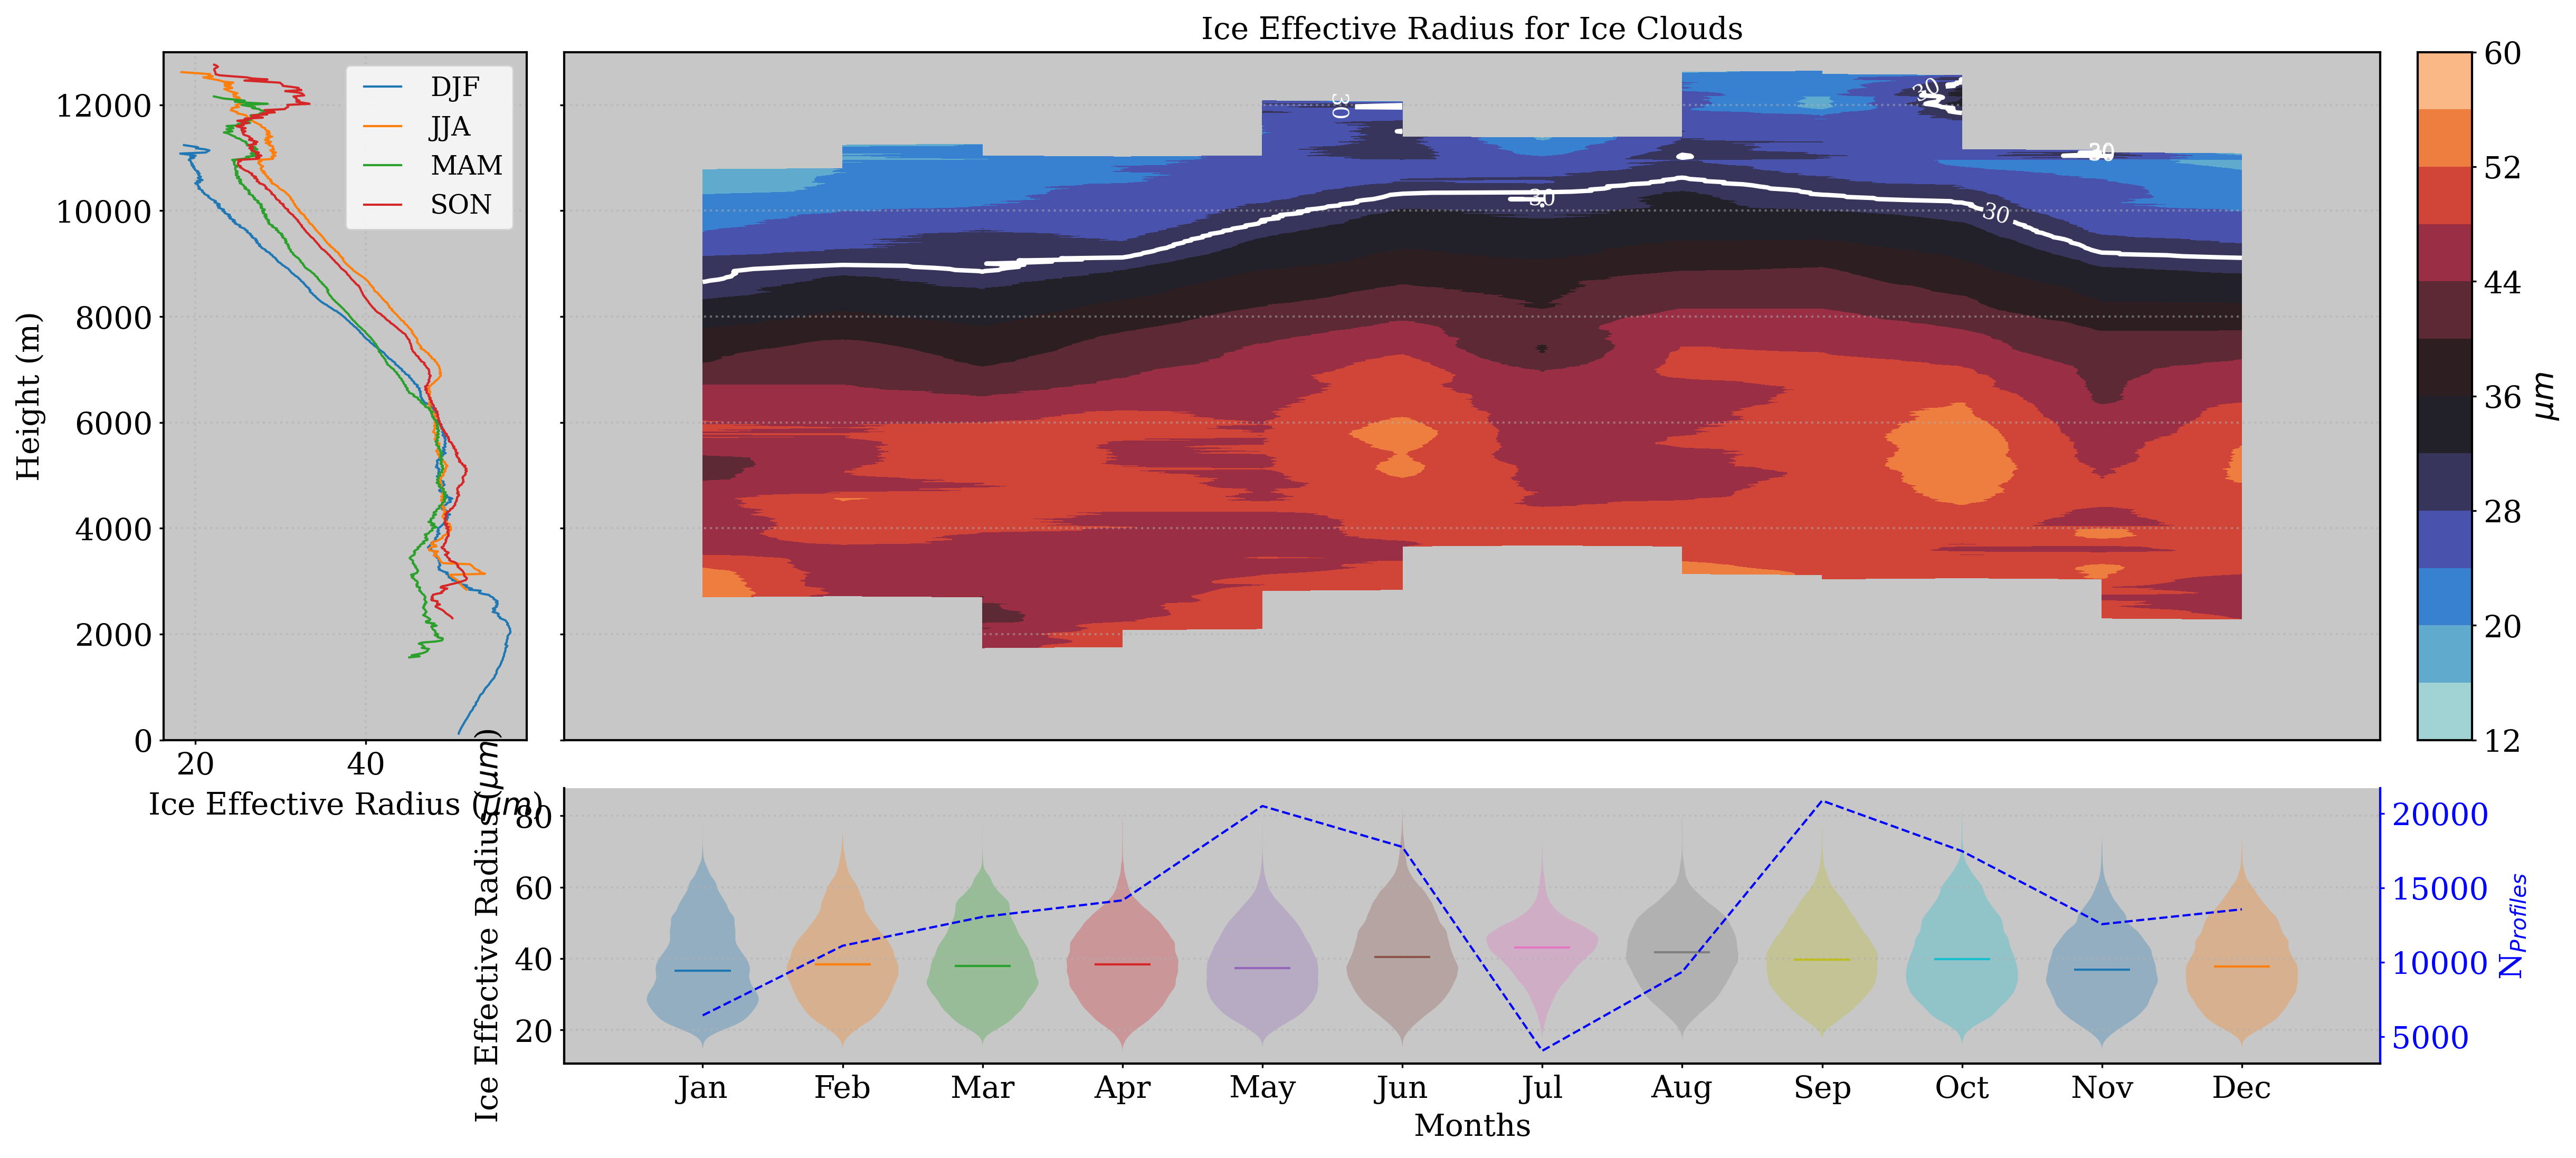
\includegraphics[width=.9\textwidth]{../../phd_clouds/figures/grouped_by_month_evolution_for_ier_Ice_mesh}
	\caption{Seasonal and monthly statistics on ice effective radius ($r_{ice}$) distribution for ice clouds. Left panel shows the seasonal median profiles of ice effective radius. Top-right panel shows the monthly profiles of the median $r_{ice}$, while the bottom-panel displays the size distribution of $r_{ice}$ by months.}
	\label{fig:IER_ice}
\end{figure}

Ice precipitating clouds are the most frequent at our station, characterized by their greater thickness and lower cloud base compared to non-precipitating ice clouds. Similar to precipitating mixed-phase clouds, these clouds possess a well-defined melting layer that separates the cloud base from rain droplets and drizzle. The highest concentrations of ice, exceeding 50 mg m$^{-3}$, are found between 2 and 5 km, with slightly elevated levels during summer and fall. Notably, regions with ice concentrations over 200 mg m$^{-3}$ were identified around 6 km in June and September, and between 9 and 12 km in July. This significant ice presence at high altitudes was not observed in ice clouds, though a relatively high ice content was detected in precipitating mixed-phase clouds in June, suggesting a correlation with the high ice amounts in summer and thicker clouds. The substantial ice amounts at high altitudes in summer are strongly linked to convective motions, providing evidence that precipitating ice clouds in summer may be associated with cumulonimbus clouds. Additionally, these clouds may represent a subsequent stage of precipitating mixed-phase clouds, exhibiting a similar pattern but with increased thickness and ice water content, particularly in summer. The left panel of Figure \ref{fig:IWC_ice_prep} illustrates similar median profiles of IWC in summer and fall, with summer displaying a secondary maximum around 11 km and fall showing a more pronounced second maximum at 13 km. In contrast, spring and winter exhibit similar maxima of 100 and 150 mg m$^{-3}$ around 4.5 km, respectively, slightly below the primary maxima of 200 mg m$^{-3}$ observed in summer and fall around 6 km. The bottom panel of Figure \ref{fig:IWC_ice_prep} highlights that these clouds contain significantly higher ice water content compared to other clouds, especially during summer and fall, with the 75th percentile increasing from 500 to 1000 mg m$^{-2}$. Furthermore, it is noteworthy that the IWP in other months is much lower, indicating that in months with a higher occurrence of these clouds, the IWP is more variable and generally smaller. The lower occurrence of warm clouds results in comparable IWC values and reduced variability.


\begin{figure}[H]
	\centering
	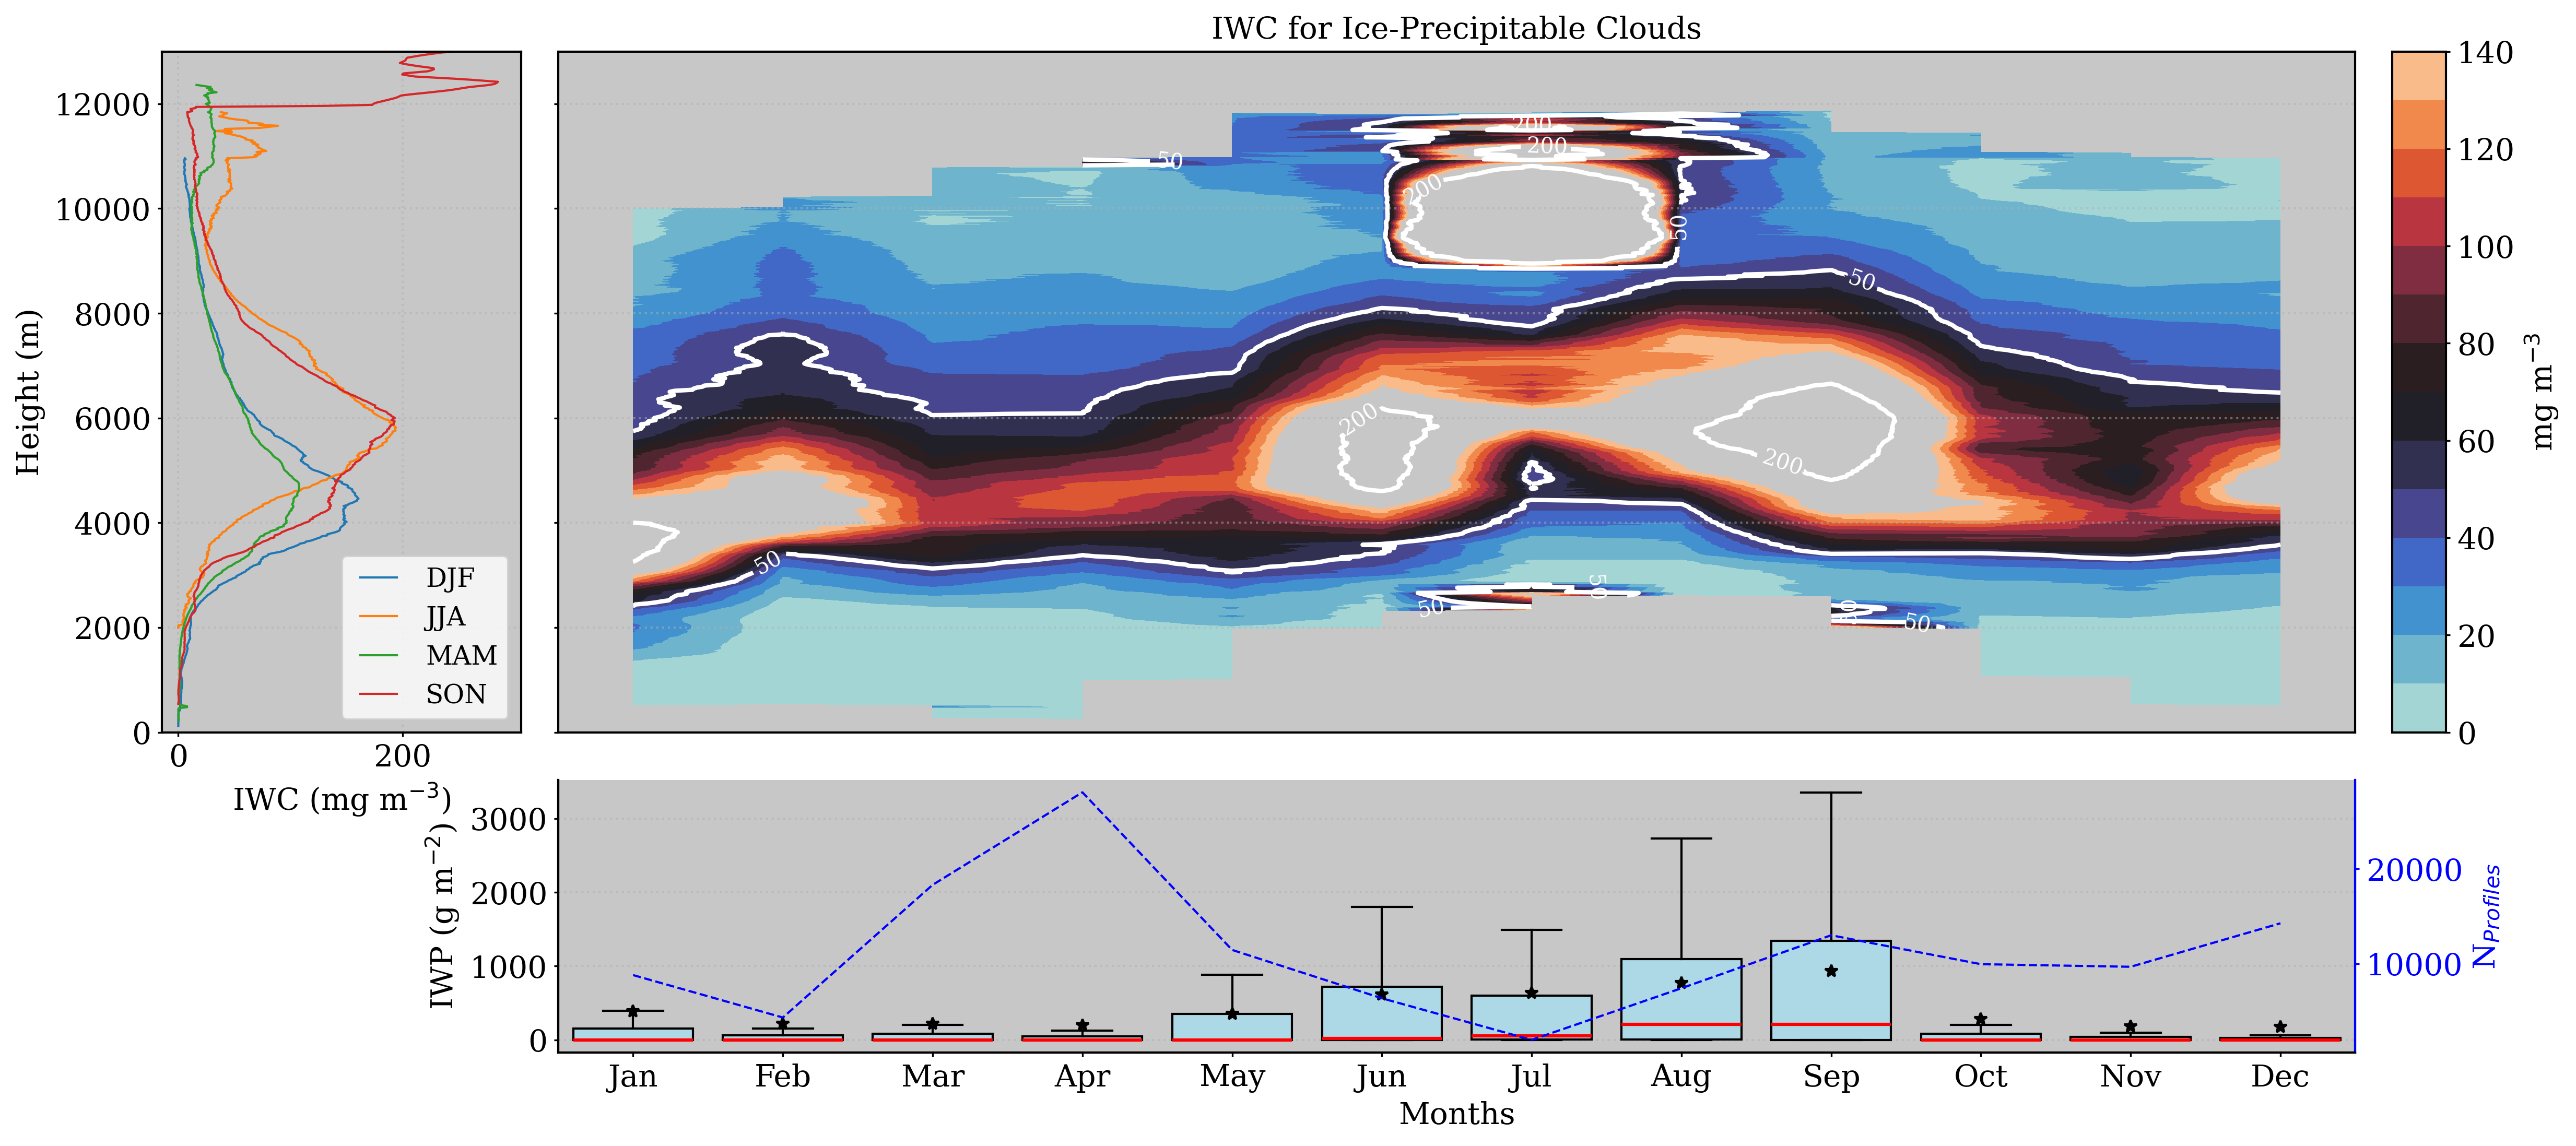
\includegraphics[width=.9\textwidth]{../../phd_clouds/figures/grouped_by_month_evolution_for_iwc_Ice-Precipitable_mesh}
	\caption{Same as Figure \ref{fig:IWC_ice}, but for ice clouds.}
	\label{fig:IWC_ice_prep}
\end{figure}

In relation to the ice effective radius ($r_{ice}$), values below 8 km range from 48 to 64 $\mu$m, with slightly larger particles observed at specific heights during winter and summer—around 5 km in winter and 7 km in summer. Notably, in summer, larger ice particles of 70 $\mu$m can be identified at 10 km, coinciding with higher ice water content (IWC). Such high values can be attributed to strong convective motions, supporting the hypothesis that these summer clouds are cumulonimbus. At the same altitude, $r_{ice}$ values in other months are generally smaller than 30 $\mu$m, except in fall, which also presents higher values at 12 km. The left panel of Figure \ref{fig:IER_ice_prep} depicts a distinct behavior of the median profiles compared to other clouds. Above 1 km, particle size begins to slowly increase (since large particles below are associated with drizzle below the cloud base). For winter and spring, $r_{ice}$ increases up to 5 km (reaching 50 $\mu$m) and then decreases to 20 and 30 $\mu$m, respectively. In contrast, for summer and fall, $r_{ice}$ increases up to 7 km (reaching 50 $\mu$m), then decreases before increasing again to reach second maxima of 50 and 63 $\mu$m, respectively. Despite the larger variability with height, the monthly distribution of $r_{ice}$ shows a highly variable pattern with a sharp mode at the median position of 50 $\mu$m.

\begin{figure}[H]
	\centering
	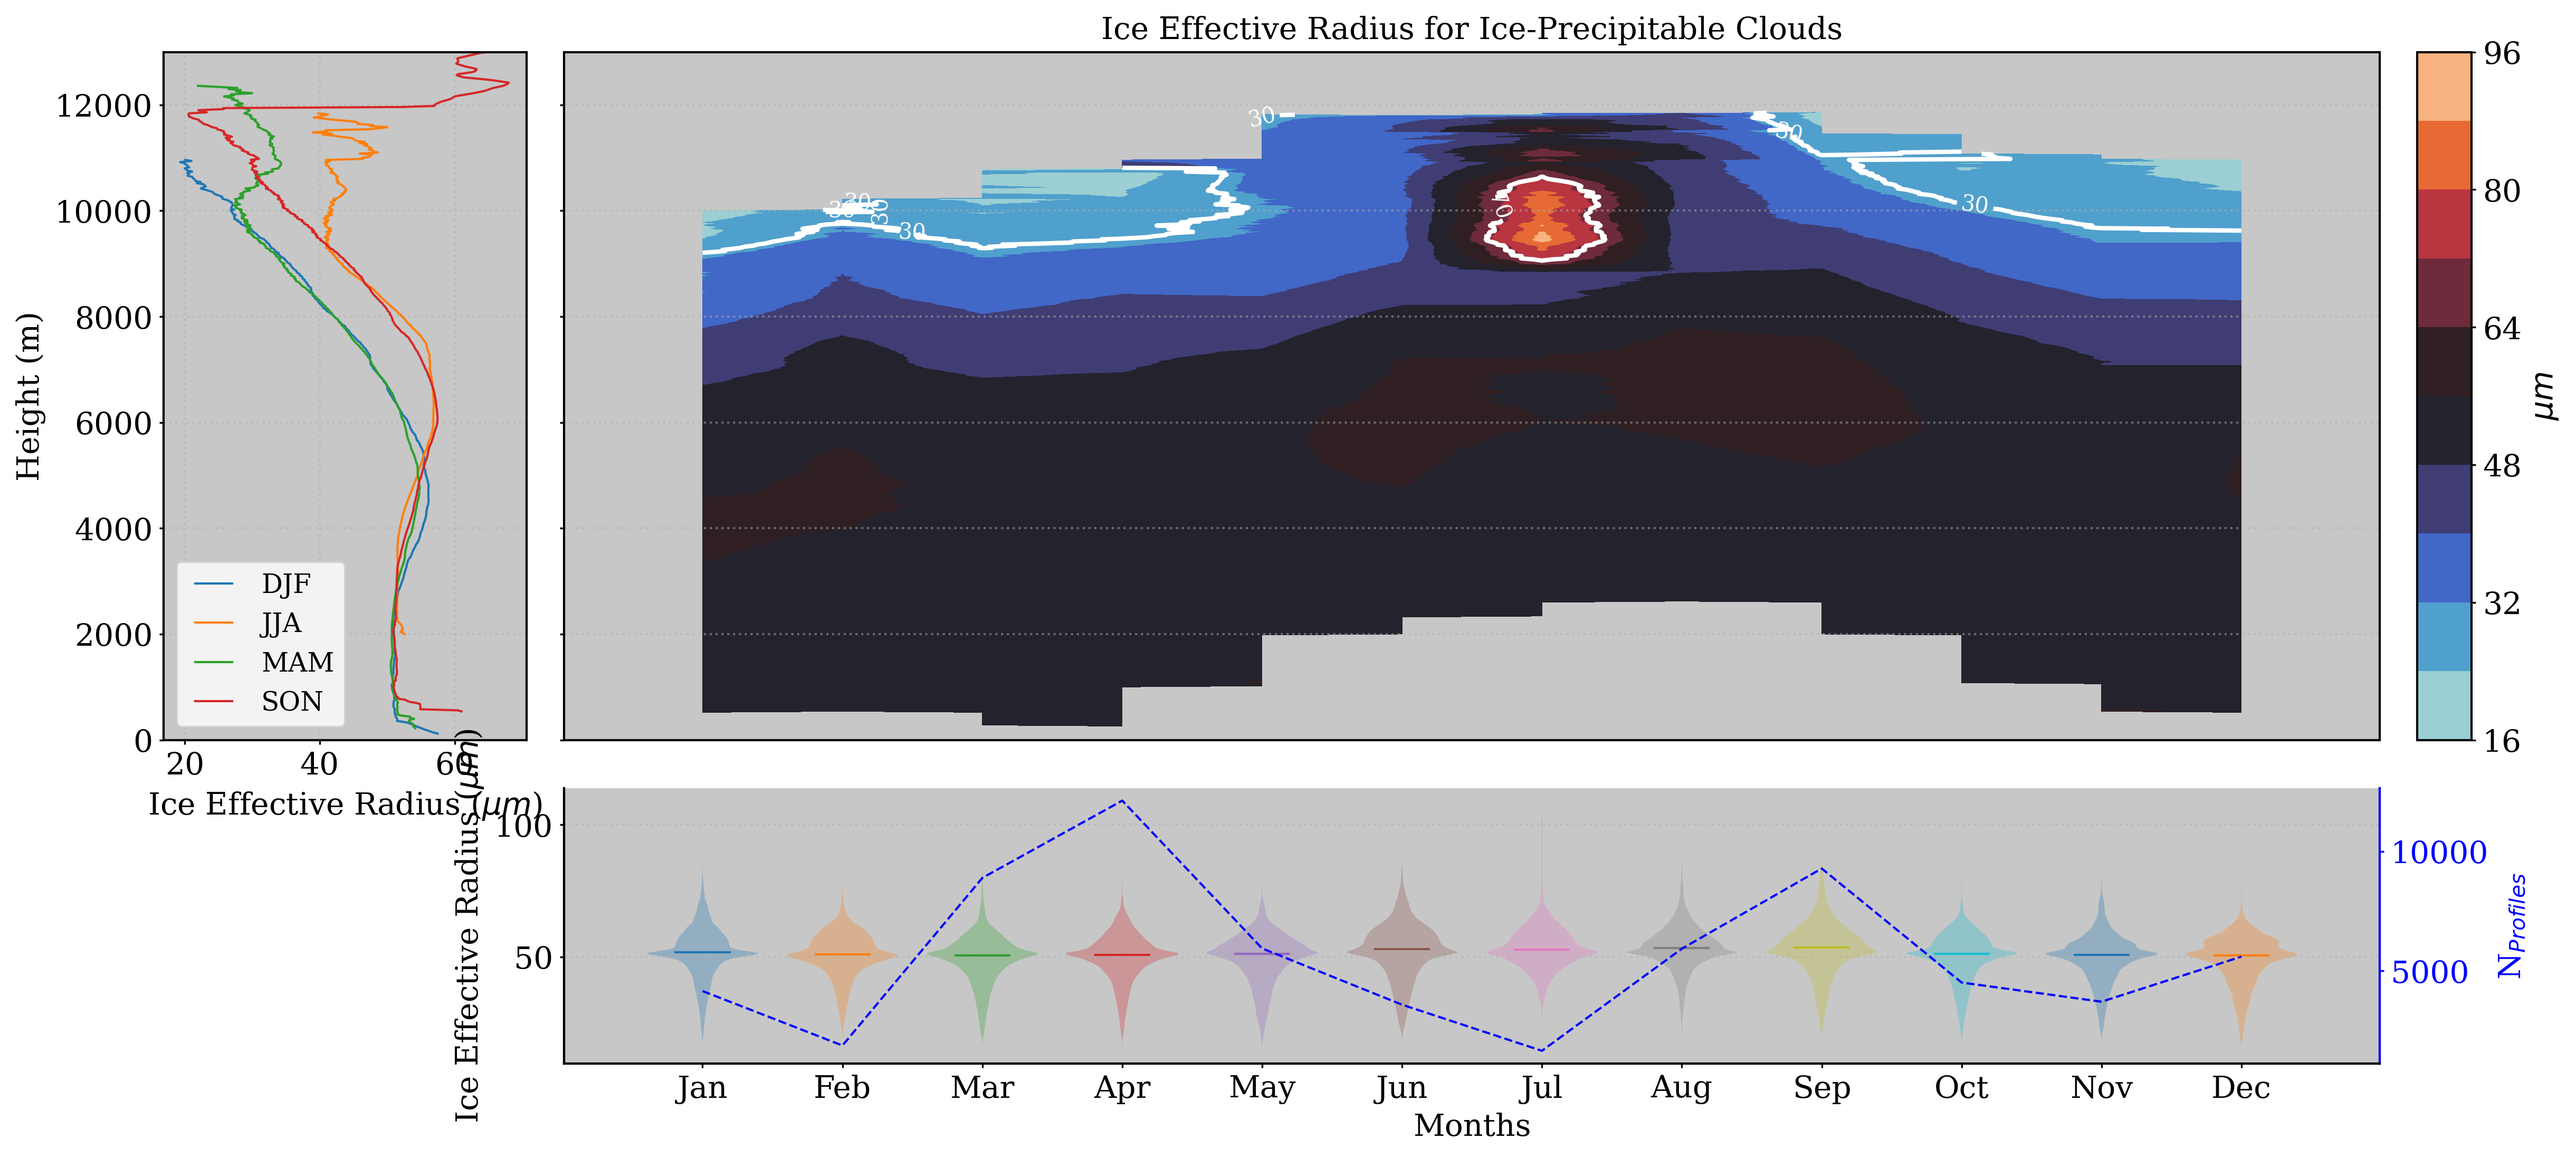
\includegraphics[width=.9\textwidth]{../../phd_clouds/figures/grouped_by_month_evolution_for_ier_Ice-Precipitable_mesh}
	\caption{Same as Figure \ref{fig:IER_ice}, but for mixed-phase clouds.}
	\label{fig:IER_ice_prep}
\end{figure}

In general, these clouds exhibit larger amounts of ice water content (IWC) at mid-levels (4-8 km), particularly in early summer and fall, while other summer months show an ice shortage. In January, most high IWC values were recorded during extreme snowfall events, such as the Filomena and Gloria storms, resulting in high median IWC at low levels during this month. The $r_{ice}$ is also influenced by these snowfalls, showing higher values close to the surface. Typically, $r_{ice}$ ranges around 50 $\mu$m up to 6 km, where it starts to decrease, indicating smaller ice particles in higher-level clouds. Precipitating mixed-phase clouds display a much stronger seasonal pattern in their physical properties. Summer and fall show a peak of IWC at 6 km, while winter and spring exhibit a less pronounced peak at 4 km. These clouds contain significantly more IWC than non-precipitating ice clouds, and they are markedly different, with greater thickness. Similar to precipitating mixed-phase clouds, they have large amounts of IWC and $r_{ice}$ at high levels in summer (> 8 km). Additionally, they demonstrate clear seasonal differences in $r_{ice}$, which is greater in summer and fall


%\section{Conclusions}
%The study of cloud coverage and its physical properties are the first step in understanding cloud radiative effects.  In order to retrieve these variables, CLOUDNET post-processed data of FMCW 94 GHz cloud Doppler radar,  HATPRO radiometer and CHM15k ceilometer were used. Additionally, complementary analysis of thermodynamic conditions was performed with the HATPRO radiometer vertical profiles. Temperature and relative humidity profiles tracked cold (fall-winter) and warm regimes (spring-summer).  
The assortment algorithm was applied using the CLOUDNET target classification product to classify different single layer cloud types. Inter-annual observation on cloud occurrence revealed a seasonal trend, where mixed phase clouds are the prevailing species, followed by ice clouds, especially during spring and winter. In these seasons, precipitating mixed phase clouds can reach 30\%XXX and 25\%XXX of frequency, respectively, and ice clouds 15\%XXX and 12\%XXX. Other cloud types have no strong seasonal pattern, and precipitating liquid clouds are absent throughout the year. In addition, the total single layer cloud frequency in summer is less than 8\%.
Mixed-phase clouds exhibit the thickest layers, followed by ice clouds and then liquid clouds. The median cloud thickness for these clouds is 2.0XXX, 1.2XXX, and 0.2XXX, respectively. However, due to their considerable variability, no distinct seasonal pattern was discernible for this property. Consequently, thicker layers of mixed-phase clouds contain more ice content than ice clouds layers. Although typical values for both are 0-20\,g~m$^{-2}$, mixed phase clouds have systematically higher IWP, with an expressive increase in fall, reaching 20-50\,g~m$^{-2}$. Conversely, liquid clouds contain slightly more liquid content than mixed-phase clouds, despite being thin. This indicates that liquid layers consistently maintain thinness, even within mixed-phase clouds. In fact, they have almost the same amount of water, within the interval of 0-20\,g~m$^{-2}$, but liquid clouds have higher probability to reach higher values, specially in spring and fall (see figure \ref{fig:LWP_hist}).

LWC and droplets effective radius does not show a clear seasonal trend for mixed and liquid phase clouds. Effective radius has almost the same distribution along year, with a median of 5\,$\mu$m for liquid clouds, and is found mainly below 3\,km. Differently mixed phase clouds have a radius that can vary a lot from the surface to 10 km, but in general, most frequent values between 5 and 12\,$\mu$m are found between 1-2 \,km and 5-9\,km. 
Concerning LWC, despite the fact that it was easy to identify higher values in cold regimes and smaller ones during summer, the variability of data goes through several orders of magnitude. It was observed for liquid and mixed phase clouds. 

With respect to ice and mixed phase clouds, the same difficulty to reach a seasonal pattern for IWC was identified. Month profiles did not show a significant difference, except that in summer, values are shifted upwards in the atmosphere. For ice clouds, effective radius can reach 65\,$\mu$m in summer, but normally they vary between 20-30\,$\mu$m around 8-12\,km.  For mixed phase clouds, ice effective radius fluctuates around 50\,$\mu$m between 1-7\,km.

Concerning cloud base height, a significantly seasonal difference on vertical distribution was observed in summer. Normally, the median value of ice cloud base height is 8\,kmXXX in fall and 7\,kmXXX for the rest of the year. For mixed phase, median values are 4\,km and 5\,km in cold and warm regimes, respectively. However, an unnusual mode around 5\,km appeared in summer, especially for mixed phase clouds, which also present a sharper distribution compared to other seasons. Nonetheless, in this season, liquid clouds presented a spreader distribution, with a median of 3\,kmXXX, against a median of 1\,kmXXX in other seasons. Cloud top height followed a simmilar behavior. In colder regimes (winter-spring), cloud top is 1.5\,kmXXX, 9\,kmXXX, 6\,kmXXX, for 
liquid, ice and mixed clouds, respectively. During warm periods (summer-fall), medians changed to 2.5\,kmXXX, 8.5\,kmXXX, 7.5\,kmXXX. However, only in summer, the meadian cloud base height for liquid clouds were 3\,kmXXX. Finally, a comprehensive analysis of cloud occurrence and physical properties was conducted at the ACTRIS-CCRESS Granada station. Notably, this is the first study on cloud properties in the southeast of Spain, an area recognized as a hotspot for climate variability. Consequently, it has the potential to enhance our understanding of global cloud properties, as the methods employed here can be applied to other stations as well.




%
%%% The following commands are for the statements about the availability of data sets and/or software code corresponding to the manuscript.
%%% It is strongly recommended to make use of these sections in case data sets and/or software code have been part of your research the article is based on.
%
%\codeavailability{TEXT} %% use this section when having only software code available
%
%
%\dataavailability{TEXT} %% use this section when having only data sets available
%
%
%\codedataavailability{TEXT} %% use this section when having data sets and software code available
%
%
%\sampleavailability{TEXT} %% use this section when having geoscientific samples available
%
%
%\videosupplement{TEXT} %% use this section when having video supplements available
%
%
%\appendix
%\section{}    %% Appendix A
%
%\subsection{}     %% Appendix A1, A2, etc.
%
%
%\noappendix       %% use this to mark the end of the appendix section. Otherwise the figures might be numbered incorrectly (e.g. 10 instead of 1).
%
%%% Regarding figures and tables in appendices, the following two options are possible depending on your general handling of figures and tables in the manuscript environment:
%
%%% Option 1: If you sorted all figures and tables into the sections of the text, please also sort the appendix figures and appendix tables into the respective appendix sections.
%%% They will be correctly named automatically.
%
%%% Option 2: If you put all figures after the reference list, please insert appendix tables and figures after the normal tables and figures.
%%% To rename them correctly to A1, A2, etc., please add the following commands in front of them:
%
%\appendixfigures  %% needs to be added in front of appendix figures
%
%\appendixtables   %% needs to be added in front of appendix tables
%
%%% Please add \clearpage between each table and/or figure. Further guidelines on figures and tables can be found below.
%
%
%
%\authorcontribution{TEXT} %% this section is mandatory
%
%\competinginterests{TEXT} %% this section is mandatory even if you declare that no competing interests are present
%
%\disclaimer{TEXT} %% optional section

\begin{acknowledgements}
TEXT
\end{acknowledgements}



%% REFERENCES

%% The reference list is compiled as follows:

%\begin{thebibliography}{}
%
%\bibitem[AUTHOR(YEAR)]{LABEL1}
%REFERENCE 1
%
%\bibitem[AUTHOR(YEAR)]{LABEL2}
%REFERENCE 2
%
%\end{thebibliography}

%% Since the Copernicus LaTeX package includes the BibTeX style file copernicus.bst,
%% authors experienced with BibTeX only have to include the following two lines:
%%
%% \bibliographystyle{copernicus}
%% \bibliography{example.bib}
\bibliographystyle{copernicus}
%\bibliography{export.bib}
\bibliography{./MyZoteroLibrary.bib}

%%
%% URLs and DOIs can be entered in your BibTeX file as:
%%
%% URL = {http://www.xyz.org/~jones/idx_g.htm}
%% DOI = {10.5194/xyz}


%% LITERATURE CITATIONS
%%
%% command                        & example result
%% \citet{jones90}|               & Jones et al. (1990)
%% \citep{jones90}|               & (Jones et al., 1990)
%% \citep{jones90,jones93}|       & (Jones et al., 1990, 1993)
%% \citep[p.~32]{jones90}|        & (Jones et al., 1990, p.~32)
%% \citep[e.g.,][]{jones90}|      & (e.g., Jones et al., 1990)
%% \citep[e.g.,][p.~32]{jones90}| & (e.g., Jones et al., 1990, p.~32)
%% \citeauthor{jones90}|          & Jones et al.
%% \citeyear{jones90}|            & 1990



%% FIGURES

%% When figures and tables are placed at the end of the MS (article in one-column style), please add \clearpage
%% between bibliography and first table and/or figure as well as between each table and/or figure.

% The figure files should be labelled correctly with Arabic numerals (e.g. fig01.jpg, fig02.png).


%% ONE-COLUMN FIGURES

%%f
%\begin{figure}[t]
%\includegraphics[width=8.3cm]{FILE NAME}
%\caption{TEXT}
%\end{figure}
%
%%% TWO-COLUMN FIGURES
%
%%f
%\begin{figure*}[t]
%\includegraphics[width=12cm]{FILE NAME}
%\caption{TEXT}
%\end{figure*}
%
%
%%% TABLES
%%%
%%% The different columns must be seperated with a & command and should
%%% end with \\ to identify the column brake.
%
%%% ONE-COLUMN TABLE
%
%%t
%\begin{table}[t]
%\caption{TEXT}
%\begin{tabular}{column = lcr}
%\tophline
%
%\middlehline
%
%\bottomhline
%\end{tabular}
%\belowtable{} % Table Footnotes
%\end{table}
%
%%% TWO-COLUMN TABLE
%
%%t
%\begin{table*}[t]
%\caption{TEXT}
%\begin{tabular}{column = lcr}
%\tophline
%
%\middlehline
%
%\bottomhline
%\end{tabular}
%\belowtable{} % Table Footnotes
%\end{table*}
%
%%% LANDSCAPE TABLE
%
%%t
%\begin{sidewaystable*}[t]
%\caption{TEXT}
%\begin{tabular}{column = lcr}
%\tophline
%
%\middlehline
%
%\bottomhline
%\end{tabular}
%\belowtable{} % Table Footnotes
%\end{sidewaystable*}
%
%
%%% MATHEMATICAL EXPRESSIONS
%
%%% All papers typeset by Copernicus Publications follow the math typesetting regulations
%%% given by the IUPAC Green Book (IUPAC: Quantities, Units and Symbols in Physical Chemistry,
%%% 2nd Edn., Blackwell Science, available at: http://old.iupac.org/publications/books/gbook/green_book_2ed.pdf, 1993).
%%%
%%% Physical quantities/variables are typeset in italic font (t for time, T for Temperature)
%%% Indices which are not defined are typeset in italic font (x, y, z, a, b, c)
%%% Items/objects which are defined are typeset in roman font (Car A, Car B)
%%% Descriptions/specifications which are defined by itself are typeset in roman font (abs, rel, ref, tot, net, ice)
%%% Abbreviations from 2 letters are typeset in roman font (RH, LAI)
%%% Vectors are identified in bold italic font using \vec{x}
%%% Matrices are identified in bold roman font
%%% Multiplication signs are typeset using the LaTeX commands \times (for vector products, grids, and exponential notations) or \cdot
%%% The character * should not be applied as mutliplication sign
%
%
%%% EQUATIONS
%
%%% Single-row equation
%
%\begin{equation}
%
%\end{equation}
%
%%% Multiline equation
%
%\begin{align}
%& 3 + 5 = 8\\
%& 3 + 5 = 8\\
%& 3 + 5 = 8
%\end{align}
%
%
%%% MATRICES
%
%\begin{matrix}
%x & y & z\\
%x & y & z\\
%x & y & z\\
%\end{matrix}
%
%
%%% ALGORITHM
%
%\begin{algorithm}
%\caption{...}
%\label{a1}
%\begin{algorithmic}
%...
%\end{algorithmic}
%\end{algorithm}
%
%
%%% CHEMICAL FORMULAS AND REACTIONS
%
%%% For formulas embedded in the text, please use \chem{}
%
%%% The reaction environment creates labels including the letter R, i.e. (R1), (R2), etc.
%
%\begin{reaction}
%%% \rightarrow should be used for normal (one-way) chemical reactions
%%% \rightleftharpoons should be used for equilibria
%%% \leftrightarrow should be used for resonance structures
%\end{reaction}
%
%
%%% PHYSICAL UNITS
%%%
%%% Please use \unit{} and apply the exponential notation


\end{document}
